
\documentclass[12pt,a4paper]{book}
\usepackage[utf8]{inputenc}
\usepackage{amsmath}
\usepackage{amsfonts}
\usepackage{amssymb}
\usepackage{graphicx}
\usepackage[left=1in,right=1in,top=1in,bottom=1in]{geometry}
%\usepackage{cite}
\usepackage[sort&compress,numbers]{natbib}
%\usepackage[minnames=2,maxnames=3,style=authoryear,backend=bibtex]{biblatex}
\usepackage{notoccite}
\usepackage{doi}
\usepackage{hyperref}
\usepackage[nottoc,notlof,notlot]{tocbibind} 
\renewcommand\bibname{References}
\usepackage[toc,page]{appendix}
\usepackage{dcolumn}% Align table columns on decimal point
\usepackage[separate-uncertainty=true]{siunitx}
%\usepackage{adjustbox}
\usepackage{rotating}
\usepackage{multirow}
\usepackage{physics}
\usepackage{mathrsfs}
%\usepackage[demo]{graphicx}
\usepackage{subcaption}
% \newcommand{\squeezeup}{\vspace{-2.5mm}}
\usepackage{setspace}
% \usepackage[bottom]{footmisc}
\usepackage{bbm}


\doublespacing
\begin{document}
%%\title{This is the title of my amazing thesis!}
%%\author{Taraneh Andalib}
%%\date{}
%%A Thesis submitted to the Faculty of Graduate Studies of \\
%%The University of Manitoba \\
%%in partial fulfilment of the requirements of the degree of

%\maketitle
\noindent
\begin{titlepage}
  \begin{center}
         \includegraphics[width=0.3\textwidth]{university.eps}\\
        \vspace*{1cm}
        
        \textbf{Magnetic Fields and Ultracold Neutron Production; }
        \\
        %\vspace{0.5cm}
        Studies Towards the Neutron Electric Dipole Moment Experiment
        at TRIUMF
        %\vspace{0.5cm}
        \\
        by\\
        
        \vspace{1.0cm}
        Taraneh Andalib
        
        %\text{Taraneh Andalib}
        \vspace{2.0cm}
        A Thesis submitted to the Faculty of Graduate Studies of\\
        \vspace{0.5cm}
        The University of Manitoba\\
        \vspace{0.5cm}
        in partial fulfilment of the requirements of the degree of
        
        \vspace{1.5cm}
        
       
        Doctor of Philosophy\\
       \vspace{0.5cm}
        
   
        \vspace{0.5cm}
        Department of Physics and Astronomy\\
        University of Manitoba\\
        Winnipeg

        \vspace{3.0cm}
        Copyright © 2018 by Taraneh Andalib
        
    \end{center}
\end{titlepage}

\renewcommand{\thepage}{\roman{page}}
\chapter*{Abstract}
The existence of a non-zero neutron electric dipole moment~(nEDM)
confirms the theoretical models of Physics beyond the Standard Model
which provide extra sources of CP violation. Based on Sakharov
Criteria, $CP$ violation is one of the main ingredients to create the
baryon asymmetry in the universe. The current upper limit of the
neutron EDM was found to be~$3.0 \times 10^{-26}$~e$\cdot$cm, which is
below the theoretical models predictions. As a result, there is a
worldwide quest to find a finite nEDM.

The typical experimental method to measure the nEDM uses the ultracold
neutrons~(UCN) and employs the Ramsey method of separated oscillatory
fields. In this method, the Larmor precession frequency of UCN is
measured in the presence of aligned Electric and Magnetic fields
orientations. Such precision measurements require high UCN statistics
and very stable and homogeneous magnetic fields.  The work presented
in this thesis is focused on the magnetic field and UCN studies for
the future nEDM measurement at TRIUMF.

The TUCAN's~(TRIUMF UltraCold Advanced Neutron source) collaboration
goal is to measure the nEDM to the sensitivity level of
$10^{-27}$. For this measurement, the~$<1$~pT magnetic stability
requirement could be met by using magnetic shields with high magnetic
permeability~($\mu$) to reduce the external magnetic fields. However,
external sources such as ambient temperature fluctuations could give
rise to a change in the magnetic properties such as $\mu$. The result
of the temperature dependence of $\mu$ measurements and related
simulations are presented here.
%The Finite Element simulations were performed to
%correlate such changes to the changes in the magnetic fields measured
%internal to the shields.
These measurements set a limit on the temperature control level for
the future nEDM measurement at TRIUMF.

The TUCAN collaboration's goal is to design a next-generation UCN
source to increase the UCN statistics and reach the required nEDM
sensitivity. In 2016, the vertical UCN source that was previously
developed at RCNP was shipped to TRIUMF. In early 2017, we
significantly improved the control system for data acquisition. In
November 2017, the first UCN experiments were conducted with the
source. The status of the current UCN facility at TRIUMF and the
result of the first UCN production tests are presented here.



%\chapter*{Acknowledgment}

%text of the acknowledgment

\cleardoublepage
%\thispagestyle{empty}
%\vspace*{\stretch{1}}
%\begin{flushright}
%\itshape
%Dedicated to myself!!
%\end{flushright}
%\vspace{\stretch{3}}
%\cleardoublepage

%\mainmatter

\tableofcontents
\listoffigures
\listoftables


%%%%%%%%%%%%%%%%%%%
%%%%%%%%%%%%%%%%%%%
%   CHAPTERS
%%%%%%%%%%%%%%%%%%%
%%%%%%%%%%%%%%%%%%%

%%%%%%%%%%%%%%%%%%%%%%%%%%%%%%%%%%%%%%%%%%%%%%%%%%%%%%%%%%%%%%
%%% THE FOLLOWING IS THE INTRODUCTION CHAPTER
%%%%%%%%%%%%%%%%%%%%%%%%%%%%%%%%%%%%%%%%%%%%%%%%%%%%%%%%%%%%%%

\chapter{Introduction\label{chap:intro}}
\renewcommand{\thepage}{\arabic{page}}% Arabic numerals for page
                                      % counter
\setcounter{page}{1}% Start page number with 1


The work presented in this thesis is focused on the important factors
for successfully measuring the neutron electric dipole moment~(nEDM)
at TRIUMF. Those two are having a very stable magnetic field
environment, as well as high ultracold neutron~(UCN) statistics. The
TRIUMF Advanced Ultracold Neutron source~(TUCAN) collaboration's goal
is to measure the nEDM to the $10^{-27}$~e$\cdot$cm sensitivity level.


This chapter provides some information on the interest in the nEDM
measurement from a physics perspective. Finding a nonzero nEDM would
answer questions regarding the matter-antimatter or baryon asymmetry
of the universe. The nEDM measurement method and a brief overview of
the UCN and nEDM facilities worldwide are also presented here.
Chapter~\ref{chap:nedm} gives a description of the future nEDM
measurement at TRIUMF and its experimental setup
components. Chapter~\ref{chap:muofT} is focused on the work towards
the temperature dependence of magnetic permeability $\mu$, which helps
to define the temperature stability requirements for the nEDM
measurement. Chapter~\ref{chap:UCNattriumf} presents the current UCN
facility at TRIUMF, where the first UCN were produced with the
vertical UCN source. Chapter~\ref{chap:UCNresult} presents the result
of those measurements with UCN. The final remarks and notes are
available in Chapter~\ref{chap:overall}.



\section{History of Fundamental Symmetries }

Studies of discrete symmetries have revealed the interactions of the
elementary particles and helped develop the underlying theories.
There are three discrete symmetries in physics: Charge
conjugation~($C$), Parity~($P$) and Time-reversal~($T$). $C$-symmetry
simply decribes physical laws under a particle-antiparticle
transformation. Parity transformation, is simply the inversion of
spatial coordinates, and Time-reversal transformation is changing the
direction of time.  Tests of Charge $C$, $P$ and $T$ symmetries
established the structure of the Standard
Model~(SM)~\cite{pospelov2005electric}.

In 1956, fall of discrete symmetries started with the famous
$\theta-\tau$ paradox in the K-mesons decay. The paradox was that two
particles previously known as $\theta^+$ and $\tau^+$, which had the
same mass and lifetime, decayed into products with different parities
\begin{equation}
  \begin{split}
    \theta^+ &\rightarrow \pi^+ + \pi^0 \\
    \tau^+ &\rightarrow \pi^+ + \pi^+ + \pi^-~.
  \end{split}
\end{equation}
At first, it was assumed that the initial states should also have
different parities, but precise measurements revealed that this is not
the case. Yang and Lee suggested that the paradox is originated from a
$P$ violation in the weak
interactions~\cite{lee1957parity}. Immediately after, an experimental
search was suggested by Ramsey for Parity violation in the $\beta$
decay of Co-60. Within a few months, $P$ violation was demonstrated by
three different experiments
~\cite{PhysRev.105.1413,PhysRev.105.1415,friedman1957nuclear}. After
the observation of $P$ violation, Landau showed that electric dipole
moments~(EDMs) are forbidden by $T$
symmetry~\cite{landau1957conservation}, and then, it was suggested
that $T$ symmetry should also be checked
experimentally~\cite{PhysRev.106.517}.
%In 1964 it was discovered that the $C$ and $P$ symmetries are broken in
%the $K$-meson decay~\cite{christenson1965regeneration}. 

One of the most fundamental symmetries in physics is
$CPT$~(Charge-Parity-Time) symmetry. The sequential operation of $C$,
$P$ and $T$ leave the system unchanged in quantum field theories. To
date, there is no experimental evindence for $CPT$ symmetry
breaking. Because of the $CPT$ invariance, breakdown of $CP$ symmetry
should be accompanied by violation of Time-reversal symmetry.

A finite EDM provides a good probe for the new sources of $CP$
violation beyond the Standard Model. EDMs caused by $CP$ violation in
the Standard Model are negligible. But most extensions of the Standard
Model~(such as supersymmetry) naturally produce EDMs that are
comparable to or larger than the present experimental limits.
% ~\cite{romalis2001new}.

The search for EDMs can be traced back to 1950, when Purcell and
Ramsey tested the possibility of finding EDMs for particles and
nuclei~\cite{PhysRev.78.807}. Smith, Purcell and Ramsey started an
experiment to search for neutron EDM $d_n$, and they achieved the
upper limit of $d_n < 5 \times 10^{-20}$~e $\cdot$
cm~\cite{smith1957experimental}.  Over the years, the upper limit on
the neutron EDM has been improved by many orders of
magnitude. Measurement of particle EDMs provide some of the tightest
constraints on the extensions to the Standard Model to probe $CP$
violation. The most recent upper limit on the neutron EDM is found to
be $\vert d_n\vert < 3.0 \times 10^{-26} $~e$\cdot$
cm~\cite{pendlebury2015revised}.



\section{Baryon Asymmetry of the Universe}
The neutron EDM provides a highly sensitive diagnostic for $CP$
violation, which is an important element for the observed
baryon asymmetry in the universe. The dominance of matter over
antimatter in the universe can be characterized by~\cite{Cline}
\begin{equation}
\eta = \frac{n_b-\bar{n_b}}{n_{\gamma}} \simeq 6 \times 10^{-10}
\end{equation}
where $n_b$ is the number of baryons, $\bar{n_b}$ is the number of
anti-baryons, and $n_{\gamma}$ is the number of photons in the cosmic
microwave backgorund.

It is possible to assume that, maybe, the universe is baryon symmetric
in a very large scale, and it is split into regions that are made of
only baryons or anti-baryons. If that was the case, an excess of gamma
rays in between these separated regions was expected to be observed
due to annihilation. But, even in the least dense regions of the
space, there are hydrogen gas clouds.

\subsubsection{Sakharov Criteria}
There are three key ingredients needed in a theory to create baryon
asymmetry known as Sakharov criteria~\cite{Sakharov:1967dj}:
\begin{center}
\begin{description}
\item[$\bullet$]Baryon number violation
\item[$\bullet$] $C$ and $CP$ violation
\item[$\bullet$] Departure from the thermal equilibrium.
\end{description}
\end{center}

The first condition is obvious because it simply means, in a reaction,
if the net baryon number is zero, there would be no baryon
asymmetry. In the reactions that violate baryon number, if there is no
$C$ and $CP$ violations, the net baryon number would be zero, and this
is because, the reactions that create excessive baryons will be
counter-balanced by the reactions that create excessive
anti-baryons~\cite{theearlyuniverse}. The third condition is essential
for a net nonzero baryon asymmetry over time, since the equilibrium
average of $B$ vanishes. Sakharov suggested that baryogenesis took
place immediately after the big bang, at a temperature not far below
the Planck scale of $10^{19}$~GeV, when the universe was expanding so
rapidly that many processes were out of thermal
equilibrium~\cite{cohen1993progress}.

\section{CP violation Beyond the Standard Model}
A testable scenario to create the baryon asymmetry in the universe is
the Electroweak Baryogenesis~(EWBG)~\cite{Morrissey2012}. The initial
condition for this process is a hot radiation-dominated early universe
with zero net baryon number. This scenario requires a first-order
electroweak phase transition in order to form bubbles of broken
electroweak phase nucleate within the surrouding plasma. The baryon
asymmetry is generated near the walls of these expanding bubbles.

EWBG satisfies all Sakharov criteria using processes that are naively
permitted in the Standard Model. However, there are two problems with
this model: the first-order first transition is not strong enough, and
it does not provide enough $CP$ violation to create the baryon
asymmetry currently observed in the universe. As a result, beyond the
Standard Model physics is necessary, such as Minimal Supersymmetric
Standard Model~(MSSM).

The $CP$ symmetry may be violated in QCD. The QCD Lagrangian consists
of two term
\begin{equation}
  \label{eqn:qcd}
\mathscr{L}= \mathscr{L}_{cp} - \theta \frac{n_f g^2}{32 \pi^2} F_{\mu \nu} \tilde{F}^{\mu \nu}~,
\end{equation}
where
$F_{\mu \nu} = \partial_\mu A_\nu + \partial_\mu A_\nu +
i[A_\mu,A_\nu]$, and
$\tilde{F}^{\mu \nu}=1/2 \epsilon^{\mu \nu \alpha \beta}F_{\alpha
  \beta}$ are the gluon field strength tensor and dual field strength
tensor respectively. The first term describes the gluons, quarks, and
their interaction, and the second term describes the interaction of
the gluons with vacuum. The existing strong bound on the
nEDM~($3 \times 10^{-26}$~e$\cdot$cm) requires the angle $\theta$ to
be very small~($\theta < 10^{-9}$). Since $\theta$ is a free
parameter, all the values between 0 and $2\pi$ are equally
likely. This is referred to as the ``Strong $CP$ problem''.

A solution to the strong $CP$ problem was proposed by Peccei and
Quinn~\cite{Peccei1977}. They proposed a new symmetry to explain the
$CP$ conservation of strong interactions, which in turn predicts a
neV~(Goldstone boson) pseudoparticle named the axion. To date the
axion has never been discovered although there is still a strong link
between axion and nEDM experiments.

\section{Neutron Electric Dipole Moment and Symmetry Breaking}
A permanent nEDM is an intrinsic property of a neutron. This
fundamental property is a measure for the separation of positive and
negative charges internal to the neutron. However, no nEDM has been
measured so far.

The interaction of the EDM $d$ of a spin-1/2 particle with the
electromagnetic field strength $F_{\mu \nu}$ in the relativistic
invariant form can be written as

\begin{equation}
\label{eqn:hamiltonianRELelectric}
H_d = \frac{d_n}{2} \bar{\psi} \gamma_5 \sigma_{\mu \nu} \psi F^{\mu \nu}~.
\end{equation}
Similarly, the interaction of a magnetic moment with the
electromagnetic field strength $F_{\mu \nu}$ is
\begin{equation}
\label{eqn:hamiltonianRELmagnetic}
  H_\mu = \frac{\mu_n}{2} \bar{\psi} i \sigma_{\mu \nu} \psi F^{\mu \nu}~.
\end{equation}

%To study the transformation properties of the Hamiltonian, it is
%interesting to see how all bilinear covariants behave under discrete
%symmetries transformation.
%In four-vector notation, the parity operator as a
%$4 \times 4$ matrix is

%\begin{equation}
%\label{eqn:parityMatrix}
%p = \left(
%  \begin{array}{cccc}
%    1 & 0 & 0 & 0 \\
%    0 & -1 & 0 & 0 \\
%    0 & 0 & -1 & 0 \\
%    0 & 0 & 0 & -1 
%  \end{array}
%  \right) ~,
%\end{equation}
%the time-reversal symmetry is
%\begin{equation}
%\label{eqn:TMatrix}
%p = \left(
%  \begin{array}{cccc}
%    -1 & 0 & 0 & 0 \\
%    0 & 1 & 0 & 0 \\
%    0 & 0 & 1 & 0 \\
%    0 & 0 & 0 & 1 
%  \end{array}
%  \right) ~.
%\end{equation}
%The transformation of all bilinear covariants is listed in
%Table~\ref{tab:transformation}.
%\begin{table}[h!]
%  \begin{center}
%    \renewcommand{\arraystretch}{2}
%\begin{tabular} {| c || c | c | c | c |} 
%  \hline
%  & current & P & C & T \\ \hline
%  \hline
%  Scalar & $\bar{\psi_1} \psi_2$ & $\eta_1 \eta_2^* \bar{\psi_1}\psi_2$ &  $\xi_1 \xi_2^* \bar{\psi_1}\psi_2$ &  $\zeta_1 \zeta_2^* \bar{\psi_1}\psi_2$ \\ \hline
%  Vector & $\bar{\psi_1}\gamma_\mu \psi_2$ &  $\eta_1 \eta_2^* \bar{\psi_1}\gamma_\mu \psi_2$ & - $\xi_1 \xi_2^* \bar{\psi_1}\gamma_\mu \psi_2$ & - $\zeta_1 \zeta_2^* \bar{\psi_1}\gamma_\mu \psi_2$ \\ \hline
%  Tensor &  $\bar{\psi_1} \sigma_{\mu \nu} \psi_2$ &   $\eta_1 \eta_2^* \bar{\psi_1} \sigma_{\mu \nu} \psi_2$ & - $\xi_1 \xi_2^* \bar{\psi_1} \sigma_{\mu \nu} \psi_2$ &  - $\zeta_1 \zeta_2^* \bar{\psi_1} \sigma_{\mu \nu} \psi_2$ \\ \hline
%  Pseuo-vector & $\bar{\psi_1} \gamma_{\mu}\gamma_5 \psi_2$ & - $\eta_1 \eta_2^* \bar{\psi_1} \gamma_{\mu}\gamma_5 \psi_2$ & $\xi_1 \xi_2^* \bar{\psi_1} \gamma_{\mu}\gamma_5 \psi_2$ &  $\zeta_1 \zeta_2^* \bar{\psi_1} \gamma_{\mu}\gamma_5 \psi_2$ \\ \hline
%  Pseudo-scalar & $\bar{\psi_1} \gamma_5 \psi_2$ & - $\eta_1 \eta_2^*\bar{\psi_1} \gamma_5 \psi_2$ & $\xi_1 \xi_2^*\bar{\psi_1} \gamma_5 \psi_2$ & $\zeta_1 \zeta_2^*\bar{\psi_1} \gamma_5 \psi_2$ \\\hline
%\end{tabular}
%\caption{Symmetry properties of all bilinear covariants  \label{tab:transformation}}
%\end{center}
%\end{table}


Assuming ${\bf{d_n}} = d_n \frac{\bf{J}}{J}$, and
$\boldsymbol{\mu_n} = \mu_n \frac{\bf{J}}{J}$ ,the interaction of a
nonrelativistic neutron with the electromagneticol field can be
described by the follwoing hamiltonian

\begin{equation}
  \label{eqn:hamiltonian}
 H= -\boldsymbol{\mu_n} \cdot \bf{B} - \bf{d}_n \cdot \bf{E}~,
 \end{equation}
where $\boldsymbol{\mu}_n$ is the magnetic moment of the neutron
interacting with the magnetc field $\bf{B}$, and $\bf{d}_n$ is
the electric dipole moment of the neutron interacting with the
electric field $\bf{E}$.

The properties of the Hamiltonian under discrete symmetries is
summarized in Table~\ref{tab:Hsymmetry}. Based on this, the first term
is $CP$-even and $T$-even, and the second term is $CP$-odd and
$T$-odd. Because of $CPT$ invariance, a nonzero EDM may exist if
both Parity and Time-reversal symmetries are broken.


\begin{table}[h!]
\begin{center}
\begin{tabular}{| l | l | l | l |} 
\hline
 & C & P & T \\ \hline
\textbf{B} & - &+ &- \\ \hline
\textbf{E} & -&- &+ \\ \hline
$\boldsymbol{\mu}$ &- &+ &- \\ \hline 
\textbf{d} & -&+ &- \\ \hline
\end{tabular}
\caption{Symmetry properties of different components of the EDM
  Hamiltonian  \label{tab:Hsymmetry}}
\end{center}
\end{table}
  
The nEDM measurement technique and a brief survey of nEDM measurements
conducted worldwide are presented in this chapter. Ultracold neutrons
are the main tool in the measurement of nEDM and their properties are
discussed below.
\section{Ultracold Neutrons\label{sec:ucnproperties}}
The measurement of the nEDM requires high neutron statistics.
Table~\ref{tab:ucnenergy} shows the various energy regimes of neutrons
and their corresponding velocities, temperatures and de Broglie
wavelengths which are related via
\begin{equation}
  \label{eqn:ucnenergy}
  E = \frac{1}{2} m v^2 = \frac{3}{2} k_B T = \frac{h^2}{2m \lambda^2}~,
\end{equation}
where $m$ is the mass of the neutron, $v$ is the neutron velocity,
$k_B$ is the Boltzmann constant, $T$ is the equivalent temperature,
$h$ is the Planck's constant, and $\lambda$ is the de Broglie
wavelength.

\begin{table}
  \centering
  \begin{tabular}{|c|c|c|c|c|}
    \hline
    Name & Energy $E$ & Velocity $v$ & Temperature $T$ & Wavelength $\lambda$ \\
    \hline
    \hline
    Fast & 10~MeV & $4.4 \times 10^7$~m/s & $7.7$~GK & 9.0~pm \\
    \hline
    Thermal & 0.0254~eV & $ 2.2 \times 10^3$~m/s & 290~K & 0.2~nm \\
    \hline
    Cold & 1~meV & 500~m/s & 8~K & 3~nm \\
    \hline
    Ultracold & 300~neV & 8~m/s & 3~mK & 50~nm \\
    \hline
  \end{tabular}
  \caption[Neutron names in different energy ranges and their
  corresponding velocities, temperatures, and wavelength]{Commonly
    used names for neutrons in different energy ranges and their
    corresponding velocity, temperature and
    wavelenght \label{tab:ucnenergy}}
\end{table}


Ultracold neutrons are neutrons with kinetic energies $\lesssim 300$~neV,
corresponding to velocities ~$\lesssim 8$~m/s, or temperatures
$\lesssim 3$~mK. UCN move so slowly that they can populate traps made
of matter, magnetic, and gravitational fields, and can be stored and
manipulated for several hundreds of seconds in such traps. Because of
their properties, UCN are a valuable tool for precise measurements in
fundamental physics.

% such as studies of quantum states of the neutron in the Earth's
% gravitational field or the measurement of the neutron EDM.
High precision studies of UCN and their interactions provide important
data for particle physics and cosmology. In addition, they enable
sensitive searches for new physics. Examples of the experiments using
UCN, which aim to discover new physics, are searches for a permanent
EDM of the
neutron~\cite{Baker2006,Serebrov2009,Lam_Gol,Altarev2010,Pendlebury2015},
precision measurements of the neutron
lifetime~\cite{pattie2018measurement,Paul2009,Wietfeldt2011,Arzumanov2000,Serebrov2005,Huffman},
and $\beta$-decay correlation
parameters~\cite{plaster2012measurement,Mendenhall,Broussard}, as well
as quests for dark matter candidates~\cite{Serebrov2008,Zimmer2010},
axion-like particles~\cite{Baessler,Serebrov2010,Afach2015}, Lorentz
invariance violations~\cite{Altarev2009}, and the measurements of the
quantum states of UCN in the gravitational field of the
Earth~\cite{Nesvizhevsky2003}.

%Among recent new topics addressed with UCN feature searches for
%‘‘mirror matter’’ as a viable candidate for dark matter, a sensitive
%test of Lorentz invariance, searches for a new fundamental force
%mediated by axionlike particles, and a demonstration of the effect of
%accelerated matter on the neutron wave.  More long-standing are
%efforts to improve the accuracy of the weak axial-vector and vector
%coupling constants of the nucleon derived from precise values of the
%neutron lifetime and the beta asymmetry, i.e., the asymmetry of
%electron emission with respect to the spin of the decaying
%neutron. These values crucially enter the calculation of reaction
%rates in big-bang nucleosynthesis and stellar fusion [16]. They are
%also applied to calculate various processes in particle physics such
%as for the calibration of antineutrino detectors, which is currently
%scrutinized in view of a ‘‘reactor antineutrino anomaly’’ hinting at
%the existence of sterile neutrinos [17,18].

The neutron is an electrically neutral hadron, and it participates in
all four fundamental interactions. As described below, UCN have
interesting kinetic energies in relation to these potential energies
of those interactions.


\subsubsection{The Gravitational Interaction}
A neutron has a mass of $m_n\approx 940$~MeV/c$^2$, and therefore, it has a
potential in the Earth's gravitational field as
\begin{equation}
V_g=mgh~.
\end{equation}
Here $h$ is the vertical displacement, and $g=9.8$~m/s$^2$ is the
acceleration due to the Earth's gravitational field.  In experiments
using thermal or cold neutrons, the effects of gravity can usually be
negligible due to the short survival times of the neutrons. However,
with the UCN experiments, since they are confined for up to several
hundreds of seconds, gravity has a significant influence.

Here
\begin{equation}
mg=102\; \text{neV/m}~,
\end{equation}
which is comparable to the UCN kinetic energy. This means, a UCN of
energy 200~neV can rise by at most 2~m.

\subsubsection{The Weak Interaction}
The weak interaction governs the radioactive $\beta$-decay of the
neutrons. A UCN decays into a proton, an electron, and an electron
antineutrino via
\label{neutrondecay}
\begin{equation}
n\longrightarrow p+e^{-}+\bar{\nu_{e}}~.
\end{equation}
The value of the neutron lifetime sets the maximum time constant with
which UCN can be stored. The current value of the neutron lifetime is
$880.2 \pm 1.0$~s~\cite{PDG2018} which is comparable to trapping times
for UCN. This sets ultimate upper bound on experiment time scale.

\subsubsection{The Electromagnetic Interaction}

Neutron is an electrically neutral, spin-1/2 particle that possesses a
magnetic dipole moment due to its internal structure, through which it
interacts with a magnetic field \textbf{B} as
\begin{equation}
  \label{eqn:vmag}
V_m=-\boldsymbol{\mu}_n \cdot \textbf{B}~,
\end{equation}
as discussed earlier, where
\begin{equation}
\vert \boldsymbol{\mu}_n \vert =60 \; \text{neV/T}~.
\end{equation}

In an inhomogeneous magnetic field, UCN experience a force described
by
\begin{equation}
  \label{eqn:fmag}
  {\bf{F}}_m = - {\boldsymbol{\nabla}V}_m = \pm \vert {\boldsymbol{\mu}}_n \vert \boldsymbol{\nabla} \bf{B}.
\end{equation}
In the nEDM measurements, the interaction of UCN with the magnetic
field is used to polarize UCN, and to measure its polarization at the
end of the measurement cycle~(see Section~\ref{sec:Ramsey}). In
Eqn.~\ref{eqn:fmag}, the sign $\pm$ corresponds to the relative
orientation between the magnetic moment and the magnetic field.  UCN
of anti-parallel spin to the magnetic field~(magnetic moment parallel)
are called ``high field seekers'', have negative $V_m$, accelerate
towards strong magnetic fields, and are attracted to it. UCN with
parallel spin~(and thus magnetic moment anti-parallel) to the magnetic
field, are called ``low field seekers'', have positive $V_m$, and
are repelled by the magnetic field.

Eqn.~\ref{eqn:fmag} is true only if UCN move adiabatically through the
magnetic field. This condition will be fulfilled when the Larmor
precession frequency of UCN is smaller than the changes in the
magnetic field in the rest fram of the UCN. However, since the UCN
have low speeds, this condition is easily fulfilled. If the UCN spin
adiabatically traces the magnetic field, it will be fully polarized,
which can be achieved by passing the UCN through a strong~$\sim 6$~T
magnetic field.

%If the magnetic field $\textbf{\textit{B}}$ is inhomogeneous and the
%neutron spin traces the magnetic field adiabatically, the neutron will
%experience a force given by:

%\begin{equation}
%\label{eqn:emforce}
%\textbf{\textit{F}}_{mag}= - \mathbf{\mathit{\nabla}} V_{mag}=\pm
%\mu_n \mathbf{\mathit{\nabla}} \vert \textbf{\textit{B(r)}} \vert.
%\end{equation}
%The neutrons that experience a force towards regions of higher
%magnetic field strength are called high-field seekers. Conversely if
%the neutrons experience a force towards regions of lower magnetic
%field (a 3D minimum in the $\textbf{\textit{B}}$ field) strength they
%are called low-field seekers. It is this force that allows UCN with
%sufficiently low energy to be confined by magnetic field gradients.
%%If the UCN spin adiabatically traces the magnetic field, it will be fully polarized
%%which can be achieved by passing UCN through a strong $\sim$~6~T magnetic field.
%Furthermore, Nuclear Magnetic Resonance (NMR) experiments can be
%conducted on UCN. For example, NMR is used to measure the EDM of
%neutrons (the Ramsey technique) where UCN are placed in aligned
%electric and magnetic fields.

\subsubsection{The Strong Interaction}
Neutrons and protons are bound in the nucleus by the strong
interaction. However, this interaction has a short range, and it only
affects the neighbouring nuclei. The Woods-Saxon potential
approximately describes the nucleons interaction inside the atomic
nucleous
\begin{equation}
  \label{eqn:woodsax}
  V(r) = - \frac{V_0}{1+\exp(\frac{r-R}{b})}~,
\end{equation}
where $V_0$ represents the potential well depth, $b$ represents the
surface thickness of the nucleus, and $R = r_0 A^{1/3}$ where
$r_0 = 1.25$~fm and $A$ is the mass number. For neutrons and protons
the depth is $V_0 \approx 40$~MeV.
%The UCN energy and their binding
%energy and the depth of the potential differ by many orders of
%magnitude.
%As a result, it is not possible to use perturbation theory
%to describe neutron scattering.
Fermi realized that it is possible to introduce an equivalent
potential which can be used to calculate the small changes in the
wavefunction outside the range of the interaction by perturbation
theory.


The scattering of a neutron from a nucleus can be described as a
superposition of an incoming plane wave and a scattered spherical
wave:

\begin{equation}
  \psi(z, \theta) = e^{ikz} + f(\theta)\frac{e^{ikz}}{z}~,
\end{equation}
where $f(\theta)$ is the angle dependent scattering amplitude and is
determined by the boundary condition at $r = R$. Since the wavelength
of the UCN is much larger than the range of the strong interaction
$R$, there is no angular momentum transfer, and the process is
dominated by the s-wave~($l = 0$) scattering. In this case, the
scattering amplitude $f$ does not depend on the incident angle
\begin{equation}
f(\theta) = const. = -a~.
\end{equation}
Since the differential cross section becomes
$\frac{d\sigma}{d\Omega} = |f(\theta)|^2 = a^2$ , where $a$ is the
scattering length, a quantity that could be experimentally measured.

The interaction of an incident neutron with a nucleus can therefore
alternatively be described by a single $\delta$-function

\begin{equation}
  V(\textbf{r}) = \frac{2 \pi \hbar^2}{m_N} a \delta^{(3)}(\textbf{r})~,
\end{equation}
where $m_N$ is the mass of neutron, and $a$ is the scattering
length. Therefore, the interaction of an incident neutron with a
liquid or a solid can be described by sum of equivalent $\delta$
functions

\begin{equation}
  \label{eqn:vFermi}
  V(\textbf{r}) = \frac{2\pi \hbar^2}{m_N} \sum_i a_i \delta (\bf{r} - \bf{r_i})~,
\end{equation}
where $r_i$ is the position of the $i$th nucleus, $a_i$ is the
scattering length with the $i$th nucleus, and the sum is over all the
nuclei. This is the Fermi pseudopotential. Because of UCN's large
wavelength, this equation can be written as
\begin{equation}
  V(\textbf{r}) = \frac{2\pi \hbar^2}{m_N}\sum_i N_ia_i\Theta(\textbf{r})~,
\end{equation}
where $N_i$ is the number density in the material i, and $\Theta(r)$
is the step function inside the domain of the material. Here the sum
is over the domains with of nuclei with the same scattering length
$a_i$. In neutron physics, this potential is typically called neutron
optical potential, since if the energy of the neutron is less than the
optical potential $E < V$, the neutron will be fully reflected from
the material surface under any angle of incidence. This sets a limit
on the UCN velocity.

UCN can be lost when reflected from the material walls.  This can be
due to the upscattering in which UCN absorb energy, or absorption in
which UCN get captured by a nucleus in the reflecting material. To
include the losses in the potential, the optical potential is usually
written as
\begin{equation}
  U(r) = V(r) - iW(r)~,
\end{equation}
where $W(r) = \Sigma N_i \sigma^i_l v$ with $N_i$ being the density,
$\sigma^i_l$ being the loss cross-section~(absorption plus inelastic
scattering) of nuclei $i$, and $v$ being the velocity. If we solve the
Schr\"{o}dinger equation with this potential, we get an additional
decay of probability density as

\begin{equation}
\rho = \rho_0 e^{-2Wt/\hbar}~,
\end{equation}
where $1/\tau_{abs} = 2W/\hbar$.  The ratio
$f = \frac{W}{V} = \frac{\sigma_l k}{4 \pi a}$ is the UCN loss
coefficient, where as earlier, $\sigma_l$ is the total loss
cross-section for neutrons with wavenumber $k$, and $a$ is the
scattering length~\cite{ucnbook}.

For almost all materials $V \gg W$. The total energy of UCN are
$E < V$ for many materials and therefore, they are reflected from
material surfaces at all angles of incidence. For $V > E$, the mean
probability of neutron loss on reflection from an abrupt potential
step~($V \gg W$), averaged over all angles of incidence, is given
by~\cite{richardson1991measurement}

\begin{equation}
  \mu(E) = 2f \left[ \frac{V}{E} \mathrm{arcsin} \left( \sqrt{\frac{V}{E}} \right) - \sqrt{\frac{\left( V - E\right)}{E}} \right]~,
\end{equation}
where $f$ is the UCN loss coefficient as described above.


The strong interaction plays a crucial role in the nEDM
measurements. Choosing certain materials enables us to store and guide
UCN to the measurement cell. The highest known value for the optical
potential is $V_F=335$~neV, and is measured for $^{58}$Ni.

%\subsection{Superthermal Sources of Ultracold Neutrons}



%The search for a nonzero neutron EDM provides a promising route to
%investigate new mechanisms of CP violation beyond the standard
%model. These in theory could help explain the matter-antimatter
%asymmetry in the Universe. At the present best level of sensitivity
%$d_n = 3.0 \times 10^{-26}$~e$\cdot$cm (90\%
%C.L)~\cite{Pendlebury2015} which was limited by counting
%statistics, severe constraints on new sources of CP violation were
%placed.

%As most other experiments with UCNs, the EDM search has been
%performed using a long-serving source~\cite{Steyerl1986} at the
%high-flux reactor of the Institut Laue Langevin (ILL) in Grenoble,
%France. It employs a neutron turbine for a phase-space transformation
%of very cold neutrons from a liquid deuterium moderator down to the
%energy range of UCN, whose high-energy limit is set by the neutron
%optical potential of the material selected for a UCN trap (such as
%252 neV for beryllium) or by the magnetic potential provided by field
%gradients in a magnetic bottle (60 neV=T). With UCN densities in the
%order of 10 per cm3 made available for experiments in a typical
%configuration of the UCN extraction from the turbine [23], the ILL
%source has defined the state of the art for more than 25
%years. However, notably,
%%%%%%%%%%%%%%%%%%%%%%%%%%%%%%%%%%%%%%%%%%%%%%%%%%%%%5
%The prospect to make an important discovery in refining the neutron
%EDM search has strongly motivated many research groups to develop next
%generation UCN sources~\cite{Golub75,Zimmer2011} which aim to
%improve the available UCN densities by more than 2 orders of
%magnitude.
%%%%%%%%%%%%%%%%%%%%%%%%%%%%%%%%%%%%%%%%%%%%%%%%%%%%%%%%%%%5
%\subsection{Properties of UCN}
%expand the first two paragraphs of Leung's paper. Also look at
%Leung's thesis.  Neutron energy and its velocity are related as
%$E_n=\frac{m_n v^2}{2}= \frac{\hbar^2 k^2}{2 m_n}=\frac{h^2}{2 m_n
%\lambda_n^2}$ where $m_n$ is the neutron mass, $v$ is the neutron
%velocity and $k=\frac{2 \pi}{\lambda_n}$ is the wave number. The
%kinetic energy is related to temperate as $E_n=k_B T_n$ where $k_B$
%is the Boltzmann constant.

%UCN have velocities less than 8~m/s and energies about 260~neV which
%corresponds to temperatures below 2~mK.  The kinetic energy of UCN is
%less than the neutron optical potential of well-chosen materials and
%so they can reflect from material surfaces at all incident angles,
%allowing them to be stored in a vessel and studied for times
%approaching the neutron lifetime.



\section{Superthermal UCN sources}
\label{sec:ucn_with_heII}



In thermal UCN sources, neutrons are extracted from a distribution
almost in thermal equilibrium with a moderation system. The UCN
turbine source at the Institute Laue-Langevin~(ILL) extracted very
cold neutrons vertically from a cold source~(liquid deuterium), and
slowed them down using the mechanical action of a
turbine~\cite{Steyerl1986,Steyerl1975}. Here cold neutrons with
velocities of $\sim$~40~m/s are decelerated by reflection from a set
of curved turbine blades moving with a velocity $\sim$~20~m/s in the
same direction as the neutrons. A UCN density of $\sim$~40~UCN/cm$^3$
was achieved with this method~\cite{ucnbook,Albert_talk}. The current
UCN density of this source is 110~UCN/cm$^3$ for neutrons with
velocities $<$~7~m/s~\cite{Steyerl1986}.


%\subsection{Goals of Superthermal UCN Sources}
In 1975 it was shown that, it is possible to achieve higher steady
state UCN densities corresponding to temperatures much lower than the
temperature of the moderator~\cite{Golub75}. These are called the
``superthermal converters''. Here thermal or cold neutrons are
inelastically scattered and transfer their kinetic energy to an
excitation of the converter medium~(e.g., to a phonon).  Superthermal
sources have the ability to provide much higher UCN densitys than
conventional sources such as the ILL turbine source. The best
candidates for the superthermal converters to date are liquid $^4$He
and solid deuterium.


%UCN are a powerful tool to study new physics and the properties of
%the neutrons.  An intense UCN beam is a common need for all of these
%experiments.  Producing a high intensity UCN source is an essential
%need for such studies.  Earlier method Before using superthermal
%converters, UCN were produced by neutron turbine
%sources~\cite{Steyerl1986,Steyerl1975}. In turbine source,
%cold neutrons with velocities of $\sim$ 40~m/s are brought into UCN
%range by reflection from a set of curved turbine blades moving with a
%velocity $\sim$ 20~m/s in the same direction as the neutrons. A UCN
%density of $\sim$30-40 UCN/cm$^3$ was achieved with this
%method~\cite{ucnbook}.

%In earlier methods of UCN production, it was assumed that the maximum
%UCN density would be achieved if the incident neutron flux is
%thermalized to the moderator~\cite{Shapiro}. The maximum
%achievable UCN density with these methods is
%$10^2-10^3$/cm$^3$~\cite{ucnbook}. The process of extracting UCN
%has a considerable degree of loss, which means, the available UCN
%will always be much less than this~\cite{ucnbook}.  The low
%density of UCN produced by thermal sources was the main constrain of
%high precision measurements such as neutron $\beta$-decay with
%UCN~\cite{Huffman} and neutron electric dipole moment
%measurement~\cite{Steyerl1986,Harris99}.

 
\subsection{Basic Idea of Superthermal UCN Sources\label{sec:basic_idea}}
The mechanism of a superthermal UCN source is the following.  An
incident neutron can lose almost its entire energy in a single
scattering event by creating excitations~( e.g., phonons) in a
converter medium~\cite{ucnbook, Golub75}. Because of the loss in the
kinetic energy, this process is called downscattering. The reverse
process is called upscattering, where a UCN absorbs kinetic energy from
the medium.


Consider a simple model for the medium as a two-level system with an
energy gap $E_0^*$. A neutron can excite a quasi-particle from the
lower state to the higher state by transferring the energy $E_0^*$. A
quasi-particle from the higher state can fall down to the lower state
by transfer of the energy $E_0^*$ to a neutron.  The principle of
detailed balance links the cross-section for upscattering
$\sigma(E_{\text{UCN}} \rightarrow E_{\text{UCN}}+E_0^*)$ and
downscattering
$\sigma(E_{\text{UCN}}+E_0^* \rightarrow
E_{\text{UCN}})$~\cite{ucnbook}

\begin{equation}
\label{eqn:detailed_balance}
\sigma(E_{\text{UCN}} \rightarrow E_{\text{UCN}}+E_0^*)= \frac{(E_{\text{UCN}}+E_0^*)}{E_{\text{UCN}}}
e^{-\frac{E_0^*}{k_B T}}\sigma(E_{\text{UCN}}+E_0^* \rightarrow E_{\text{UCN}})
\end{equation}
where $T$ is the temperature of the medium, $E_{\text{UCN}}$ is the
energy of the UCN, and $k_B$ is the Boltzmann constant.

In general, $\sigma(E_{\text{UCN}}+E_0^* \rightarrow E_{\text{UCN}})$
is practically independent of $T$, so that for
$E_0^* \gg k_B T \gg E_{\text{UCN}}$, the upscattering cross-section
for UCN can be made arbitrarily small by decreasing the
temperature. If the converter is now placed in a neutron flux at a
temperature $T_n \geq E_0^*$, there will be a significant number of
downscattering events, and a negligible number of upscattering events.

If the converter is contained in a vessel whose walls are good UCN
reflectors with potential $V \gg V_m$, where $V_m$ is the UCN potential
of the converter, and the walls are transparent to the neutrons of
energy $E_0^*$, then UCN will build up in the moderator to a density
until the rate of loss is equal to the rate of UCN production.

%Coherent inelastic scattering can provide the equivalent of a
%two-level system for UCN \cite{ucnbook}.  A neutron at rest can
%only absorb a phonon with energy E$_0^*$ and a neutron with
%E$>$E$_0^*$ can come to rest by emitting a phonon with energy
%E$_0^*$.  The upscattering process is suppressed by a Boltzmann
%factor $e^{-E_0^*/{k_BT}}$. If the medium is sufficiently cold and
%the excitation energy introduced by the neutrons can be cooled away,
%upscattering becomes negligible.  If the converter is at thermal
%equilibrium at temperature $T$, then $E_0^* \gg k_B T \gg E_{\text{UCN}}$
%where $E_{\text{UCN}}$ is the UCN energy. Only neutrons with energies close
%to $E_0^*$ can scatter in the converter medium. In addition, the UCN
%bottle wall has to have a much higher effective potential than the
%converter medium to prevent UCN loss.

The steady-state UCN density in the source is given by
\begin{equation}
\label{ucndensity}
\rho_{\text{UCN}}=P_{\text{UCN}} \tau,
\end{equation}
where $P_{\text{UCN}}$~(UCN/cm$^3 \cdot$s) is the UCN production rate,
and $\tau$~(s) is the UCN mean lifetime in the system.  The mean
lifetime $\tau$ of the UCN in the vessel is restricted by a variety of
possible loss mechanisms
\begin{equation}
\frac{1}{\tau} = \frac{1}{\tau_a}+ \frac{1}{\tau_W}+\frac{1}{\tau_{up}}+\frac{1}{\tau_{\beta}},
\end{equation}
where $1/\tau_a$ is the UCN absorption rate in the medium, $1/\tau_W$
is the rate of the UCN loss on the walls, $1/\tau_{up}$ is the neutron
loss due to the upscattering in the medium, and $1/\tau_{\beta}$ is
the $\beta$-decay losses.

%An important factor in choosing a UCN source is the absorption rate of the neutron. As a result, pure
Pure deuterium and liquid $^4$He are good candidates for superthermal
conductors, possessing a balance of high production rate, and small
neutron absorption cross-section, and upscattering rate.


\subsection{UCN Production by Superfluid $^4$He}

\subsubsection{Superfluid $^4$He Definition}

$^4$He is an isotope of helium with two protons and two neutrons. It
has an integer spin of zero, which makes it a boson. As a result, it
follows the Bose-Einstein statistics. It has two liquid states known
as He-I and He-II. The He-I phase is the normal fluid phase. The He-II
phase can be described by the so-called ``two-fluid model'', which
consists of normal liquid helium and superfluid helium.
% with zero viscosity, and zero entropy.
Fig.~\ref{fig:phasetransition} shows the phase transition diagram of
$^4$He. The two phases are separated out by the $\lambda$-line. The
phase transition happens at 2.172~K. Below 1~K, the liquid is mostly
the superfluid component of the two-fluid model.

In this thesis, I use the term ``superfluid helium'' generally to
refer to He-II cooled significantly below the lambda point, which is
nearly synonymous with that component of the two-fluid model.

\begin{figure}[h!]
  \centering \includegraphics[width=0.7\textwidth]{phasetransition.png}
  \caption[Phase diagram of $^4$He]{The phase diagram of $^4$He. Here
    the normal fluid phase or He-I and the superfluid phase or H-II
    are shown.}
\label{fig:phasetransition}
\end{figure}

Because of its zero viscosity, superfluid helium has the ability to
flow through very small capillaries or narrow channels without
experiencing any friction at all. The climbing of He-II along the
surface is called ``film flow''.


\subsubsection{Superfluid Helium Converter}

Superfluid $^4$He is an attractive candidate as a UCN source, and was
studied in Ref.~\cite{Golub77}. The dominant production mechanism in
the superfluid helium is the excitation of a single phonon at the
crossing of the free neutron and phonon dispersion curves, with a
momentum $q\sim 0.7$/\AA~\cite{Brome2001}, and energy 1~meV
corresponding to a neutron wavelength 8.9~\AA. The availability of
8.9~\AA~cold neutrons is crucial and their flux must be maximized. In
superfluid helium, the upscattering losses become smaller than
$\beta$-decay losses below $T \sim 0.7$~K. It has zero neutron
absorption cross-section, resulting in $\tau_a \rightarrow \infty$,
which makes it a good candidate as a UCN source.

%For a long UCN lifetime in superfluid helium, besides the low
%temperature of the converter, the $^3$He contamination must be low
%($^3$He/$^4$He $\le 10^{-12}$), due to its large absorption
%cross-section, which requires $^4$He purification.
There are two types of UCN sources based on superfluid helium: sources
where experiment and source are combined in one apparatus, and the
measurement is performed inside the superfluid helium, and
extracted-UCN sources where the source is an apparatus on its own, and
delivers neutrons to experiments at room temperature connected to it
by UCN guides.



\subsubsection{UCN Production Rate with Single Phonon scattering in
  Superfluid
  helium\label{sec:UCN_production}}
UCN can be produced in superfluid helium when the energy of the
incident neutrons is equal to that of the one phonon excitation in the
converter medium~\cite{Korobkina2002,Schmidt2009,Golub77}. The
incident neutrons then scatter down to UCN in the converter medium
while creating a phonon.
%The crossing of the dispersion curve for excitations in superfluid
%helium and the free energy of the neutron shows that the neutron
%wavelength should be 0.89~nm~\cite{Brome2001} or 8.9~\AA ~in
%order to excite phonon transitions.
\begin{figure}[h!]
\begin{center}
   \includegraphics[width=0.7\textwidth]{FIG1_2.PNG}
   \caption[Free neutron and superfluid helium dispersion
   relation]{\cite{PSI_news} Dispersion relation of superfluid
     helium~(c) and of the free neutron~(a). Neutrons with
     $E\simeq 1$~meV and wavenumber $q \simeq 0.7$/\AA~can excite a
     single phonon with the same energy and momentum and be
     downscattered to UCN energy range. The UCN production rate
     (b)(circles) shows the dominance of this single phonon process
     with respect to multiphonon processes at higher momentum $q$.
%    The two curves cross at $q=0$ and at $q=q^*$, which corresponds
%    to a neutron wavelength of 0.89~nm, oe an energy of 12~K.
    }
%     \vspace{-2.em}
    \label{fig:FIG1}
    \end{center}
\end{figure} 
Fig.~\ref{fig:FIG1} shows the dispersion relation of the superfluid
helium and a free neutron. A neutron at rest can absorb energy $\hbar
\omega$ and momentum $\hbar q$ with
\begin{equation}
\label{neutron_energy}
\omega=\frac{\hbar q^2}{2m}~,
\end{equation}
where $m$ is the mass of the neutron. A neutron with this energy and
momentum can come to rest after transferring its energy and momentum
to the superfluid $^4$He. For single phonon interactions, which are
usually dominant, the superfluid helium can only exchange quantities
of energy and momentum that are related by the dispersion curve

\begin{equation}
\label{dispersion_helium}
\omega=\omega(q) \simeq cq~,
\end{equation}
where $\omega$ is the energy of the phonon, $q$ is the phonon's
momentum, and $c$ is the speed of sound in the moderator. Here an
approximation is used to simplify the discussion. The neutrons can
only come to rest by emission of a single phonon, if they have the
resonant energy $E_0^*$ given by the intersection of
Eqns.~(\ref{neutron_energy}) and (\ref{dispersion_helium})

\begin{equation}
\omega(q)=cq=\frac{\hbar q^2}{2m}~,
\end{equation}
and so
\begin{equation}
q^*=\frac{2mc}{\hbar}~.
\end{equation}

%Fig.~\ref{fig:FIG1} shows that an incident neutron can lose its
%entire energy by creating a phonon excitation inside the converter
%medium if it has the energy amount equal to the phonon excitations in
%the converter medium. If this energy is $E_0^*=\hbar^2 k_0^*/2m$,
%using Eqns.~(\ref{dispersion_helium}) and~(\ref{neutron_energy}),
%$k_0^*=2mc/ \hbar$.

The differential cross-section for neutron scattering is given by the
dynamic scattering function $S(q,\omega)$, which is the Fourier
transform of the Van Hove correlation function $G(r,t)$ in space and
time of the superfluid helium~\cite{Squires}:

\begin{equation}
\frac{d\sigma}{d\omega}=b^2 \frac{k_2}{k_1}S(q,\omega) d\Omega,
\end{equation}
where $b$ is the bound neutron scattering length for $^4$He,
$\hbar k_1$ is the momentum of the incident neutrons, and
$\hbar k_2=\hbar k_{\text{UCN}}$ is the momentum of the UCN. The
quantity $S(q,\omega)$ has been measured in great
detail~\cite{S_func1,gibbs1999collective,S_func3}. Performing the
change of variables,

\begin{equation}
d\Omega=2 \pi \sin \theta d \theta = 2 \pi \frac{q dq}{k_1 k_2}
\end{equation}
gives

\begin{equation}
 \frac{d\sigma}{d\omega}=2\pi b^2 \frac{k_2}{k_1}S(q,\omega)\frac{q
   dq}{k_1 k_2}=2\pi b^2 S(q,\omega)\frac{q dq}{k_1^2}~.
\end{equation}
This may effectively be integrated over the limits on $q$ which are

\begin{equation}
  k_1-k_2 < q < k_1+k_2~.
\end{equation}
Since
\begin{equation}
k_2=k_{\text{UCN}} \ll k_1~, \; \; q\sim k_1~,
\end{equation}
we may write $dq=2k_{\text{UCN}}$. This results in the cross-section
being related to $S(q,\omega)$ evaluated on the incident neutron's
dispersion curve:

\begin{equation}
\frac{d\sigma}{d\omega}=4\pi b^2 \frac{k_{\text{UCN}}}{k_1}S \left(
k_1, \omega=\frac{\alpha k_1^2}{2} \right),
\end{equation}
where $\alpha=\frac{\hbar}{m}=4.14$~meV/\AA$^2$, and $S(q,\omega)$
assumed to be constant over the narrow range $dq$. The approximation

\begin{equation}
\omega=\frac{\hbar (k_1^2-k_2^2)}{2m}=\frac{\alpha}{2} (k_1^2 -
k_2^2)\approx \frac{\alpha}{2}k_1^2
\end{equation}
has also been used.

The UCN production rate is given by
\begin{equation}
\label{UCN_production}
P(E_{\text{UCN}}) dE_{\text{UCN}} = N_{\text{He}} \int \frac{d\Phi
  (E_1)}{dE}\cdot \frac{d \sigma}{d \omega}(E_1 \rightarrow
E_{\text{UCN}}) dE_1 dE_{\text{UCN}}~,
\end{equation}
where $\frac{d\Phi (E_1)}{dE}$ is the differential incident neutron
flux, $N_{\text{He}}$ is the atomic density in the liquid helium, and
$\frac{d \sigma}{d \omega}(E_1 \rightarrow E_{\text{UCN}})$ is the
energy differential cross-section for the inelastic neutron scattering
or the probability of the incident neutrons with energy $E_1$ to
scatter from the helium nucleus and become UCN.  Then

\begin{equation}
\label{eqn:He_P_rate}
\begin{split}
\int _0 ^{E_c} P(E_{\text{UCN}})dE_{\text{UCN}} &= N_{\text{He}} 4 \pi b^2
\alpha^2 \left[ \int \frac{d\Phi(k_1)}{dE} S \left( k_1,
  \omega=\frac{\alpha k_1^2}{2} \right)dk_1 \right] \int_0^{k_c}
k_{\text{UCN}}^2dk_{\text{UCN}} \\ &=N_{\text{He}} 4 \pi b^2 \alpha^2 \left[
  \int \frac{d\Phi(k_1)}{dE} S \left( k_1, \omega=\frac{\alpha
    k_1^2}{2} \right) dk_1 \right] \frac{k_c^3}{3}\;
\text{UCN}/\text{cm}^3 \text{s},
\end{split}
\end{equation}
where $E_c$ and $k_c$ are the critical UCN energy and wave vector of
the walls of the storage chamber. This way of writing the UCN
production rate is more general, and it is useful to calculate the
single phonon and multiphonon contributions to the UCN production
rate. The one phonon production rate is found by evaluating
Eqn.~(\ref{eqn:He_P_rate}) over the one phonon peak ($q^*=0.7$/\AA).
Thus
\begin{equation}
P_{\text{UCN}}=9.44 \times 10^{-9}\frac{d\Phi (E_1^*)}{dE_1^*} \;
\text{UCN}/\text{cm}^3,
\end{equation}
 where $E_1^*$ is the energy of the incident neutrons at the one phonon peak.
%\begin{equation} P_{1p}=N4\pi b^2 S^* \alpha \beta
%\frac{k_c^3}{3k^*}\frac{d\Phi (E_1^*)}{dE} \; \text{UCN}/\text{cm}^3
%, \text{s} \end{equation}





% The differential cross-section $\frac{d \sigma}{d E_{UCN}}$ is given
% by \begin{equation} \label{energy_differential_cross_section}
% \frac{d\sigma}{d E_{UCN}}= 4 \pi b^2 \frac{k_{\text{UCN}}}{k_0}S(q,
% \omega) \end{equation} where $b$ is the bound neutron scattering
% length for $^4$He, $k_{\text{UCN}}$ is the UCN momentum and $S$ is
% the Fourier transform of the Van Hove correlation function $G(r,t)$
% in space and time of the superfluid helium~\cite{Squires}.
% Here \begin{equation}
% \omega=\frac{E_0-E_{UCN}}{\hbar} \end{equation} but since $E_0 \gg
% E_{UCN}$, then \begin{equation} \omega \simeq
% \frac{E_0}{\hbar} \end{equation}
% and, \begin{equation} \label{wave_vector_transfer} k_0 -
% k_{\text{UCN}} < q < k_0 + k_{\text{UCN}} \end{equation} where
% $k_{\text{UCN}} \ll k_0$ and therefore $q \simeq k_0$. Therefore
% $\omega=\frac{\alpha k_0^2}{2}$ where $%
% \alpha=\frac{\hbar}{m}=4.14$ meV \AA$^{-2}$. By substituting
% Eqn.~(\ref{energy_differential_cross_section}) to
% Eqn.~(\ref{UCN_production}), the general form of UCN production rate
% will be

% \begin{equation} \label{UCN_Production_rate_helium} P(E_c)= N_{\text{He}} 4
% \pi b^2 \alpha^2 \left[ \frac{d\Phi (k_0)}{dE} S(k_0,\omega) dk_0
% \right] \frac{k_c^3}{3} \end{equation} with the units of UCN
% cm$^{-3}$s$^{-1}$ \cite{Korobkina2002}. $E_c$ and $k_c$ are the
% critical UCN energy and wave vector of the walls of the storage
% chamber.  The UCN density produced by one-phonon excitation in
% superfluid helium was first calculated by Golub and Pendlebury
% \cite{Golub77}. They found a UCN density of $\rho_U\simeq 300$
% n~cm$^{-3}$ for a cylindrical bottle with radius 10 cm and diameter
% 20 cm. This was a substantial improvement over all existing UCN
% sources which yield $\rho\lesssim 1$ n~cm $^{-3}$.

%To achieve such UCN density, the density of $^3$He must be low enough
%so that the neutron absorption by $^3$He does not significantly
%affect the storage time in the vessel.

%In the first UCN production, the UCN output was a factor of 50 lower
%than expected \cite{Ageron1978}.  The UCN production rate (first
%calculated by Pendlebusyin 1982)can be calclated by evaluating
%Eqn.~(\ref{UCN_Production_rate_general}) over the one phonon peak
%which is at $k_0^*=0.7 \AA ^{-1}$.

% \begin{figure}[h!]  \begin{center}
% \includegraphics[width=0.5\textwidth]{FIG1.PNG} \caption{The
% dispersion curve for excitations in superfluid helium and the free
% energy of the neutron as a function of momentum transfer
% $q$~\cite{Brome2001}. The two curves cross at $q=0$ and at
% $q=q^*$, which corresponds to a neutron wavelength of 0.89~nm, oe an
% energy of
% 12~K.}  \vspace{-2.em} \label{fig:FIG1} \end{center} \end{figure}



% \item[$\bullet$] why helium? (small neutron absorption cross-section
% ) \item[$\bullet$] UCN production rate in superfluid He calculation
% (Golub77) \item[$\bullet$] Experiment shows the production rate
% matches theory (Ageron1978) and recent UCN rates
% (Zimmer2011) \item[$\bullet$] Experiment design (for example ILL
% design Baker 2003, Masuda2002, PSI source
% Anghel2009) \item[$\bullet$] Temperature of the helium source,
% (below 1K Masuda2012 )

% \item[$\bullet$] UCN storage time in superfluid helium (Golub79)
% \begin{description}

%%%%%%%%%%%%%%%%%%%%%%%%%%%%%%%%%%%%%%%%%%%%%%%%%%%%%%%%%%%%%%%%%
%%   FOURTH EDIT UP TO HERE
 %%%%%%%%%%%%%%%%%%%%%%%%%%%%%%%%%%%%%%%%%%%%%%%%%%

 \subsubsection{Multiphonon Scattering Contribution in UCN Production
   in Superfluid helium}
%So far, the UCN production was demonstrated by single phonon emission. Even though one phonon emission is the predominant process in UCN production for a monochromatic UCN beam, the
 For polychromatic neutron sources, UCN can also be produced by
 multiphonon processes in superfluid
 $^4$He~\cite{Korobkina2002,Schmidt2009}. Multiphonon production of
 UCN with various energy spectra of the neutron flux has been studied
 in Ref.~\cite{Korobkina2002}.  Fig.~\ref{fig:Korobkina2002} shows the
 energy spectra $\frac{d\phi}{dE}$ for three sources as a function of
 momentum $q$, compared to the dynamic scattering function
 $S(q,\omega=\hbar q^2/2m)$. The peak at $q=0.7$/\AA~in the dynamic
 scattering function corresponds to the one phonon excitation by
 superfluid helium. The values of $S$ above 1.2/\AA~are
 extrapolated. The value of $S$ above 2/\AA~are essentially zero.  The
 UCN production from one phonon and multiphonon processes have been
 calculated for three input neutron spectra: SNS ballistic guide,
 PULSTAR MC flux and HMI polarized flux.  The multiphonon contribution
 to the UCN production is calculated using Eqn.~(\ref{eqn:He_P_rate}),
 and calculating
 $\int \Phi(E_1)S(k_1,\omega=\frac{\alpha k_1^2}{2}) dk_1$.  The
 result showed that, for sources where He-II is exposed to the total
 thermal flux or at a dedicated spallation source, the multiphonon
 contribution can amount to slightly more than a factor of 2 increase
 in the UCN production.





\begin{figure}[h!]
\begin{center}
   \includegraphics[width=0.7\textwidth]{Korobkina2002.PNG}
   \caption[Cold neutron energy spectrum and $S$ function]{The energy
     spectrum of the incident cold neutron flux from three sources
     compared to the dynamic scattering function
     $S(q,\omega=\frac{\alpha k_1^2}{2})$~/meV as a function of
     $q$~/\AA.}
%     \vspace{-2.em}
    \label{fig:Korobkina2002}
    \end{center}
\end{figure} 



%They took the energy spectrum of the neutron flux from three sources
%and extrapolated it for values of $q > 1.2$ \AA $^{-1}$ and they
%compared the results to the scattering function.

%The proposed UCN source at the North Carolina State (NC) locates a
% UCN source in the thermal column of the campus 1-MW PULSTAR reactor
% after removing the graphite. The main point of this design was the
% independence of the UCN production process to the direction of the
% incident neutrons. The proposed UCN source at the Spallation Neutron
% Source (SNS) places a superthermal UCN source on a monochromatic
% 0.89~nm beam at a guide tube. Two types of guides as ``ordinary''
% supermirror guide and ``ballistic'' guide. The ballistic guide has
% more flux at the critical 0.89~nm wavelength but less flux at
% wavelengths shorter than 0.6~nm.  The results are summarized in
% Table~\ref{tab:multiphonon}.  \begin{table} \begin{center} \begin{tabular}{|c|c|c|c|c|c|}
% \hline & NC state & SNS ord & SNS ball & HMI a.u. & Maxwell
% \\ \hline Multi-ph & 490 & 1.0 & 0.94 & 4.7 & 1.7\\ \hline Single-ph
% & 375 & 1.8 & 2.4 & 5.5 & 1.5 \\ \hline Mph/1ph & 1.4 & 0.55 & 0.4 &
% 0.85 & 1.13 \\ \hline \end{tabular} \caption{Predicted production
% rates of UCN from single and multiphonon emission from three sources
% and comparison to Maxwellian
% spectrum} \label{tab:multiphonon} \end{center} \end{table} For the
% NC state proposed UCN source, where the helium is exposed to the
% total thermal flux, the inclusion of multiphonon contribution
% increases the UCN production rate by a little more than a factor of
% 2.

%%%%%%%%%%%%%%%%%%%%%%%%%%%%%%%%%%%%%%%%%%%%%%%%%%%%%%%%%%%%%%%%%%%%%%%%%%%%%%
%% I can get rid of this part
%%%%%%%%%%%%%%%%%%%%%%%%%%%%%%%%%%%%%%%%%%%%%%%%%%%%%%%%%%%%%%%%%%%%%%%%%%%%%%
UCN production by multiphonon excitation in superfluid helium under
pressure was studied in Ref.~\cite{Schmidt2009}.  The dynamic
scattering function $S(q,\omega)$ of the superfluid helium strongly
depends on pressure, leading to a pressure-dependent differential UCN
production rate. The expression for the multiphonon part of $S$
describing UCN production is derived from the inelastic neutron
scattering data.  Application of pressure to superfluid helium
increases the velocity of sound, such that the dispersion curves of
the $^4$He and of the free neutron cross at shorter neutron
wavelength.

Since for neutron beams from a liquid deuterium cold source, the
differential flux density $\frac{d\Phi}{dE}$ in the range
8-9~\AA~normally increases for decreasing wavelength of the cold
neutron flux, and also since pressure increases the density of He-II,
it was expected to observe an increase in the single phonon UCN
production rate, and different multiphonon contribution with pressure
increase.  It was observed that, both the single and the multiphonon
scattering functions change with pressure. The single phonon
excitation moves to a shorter wavelength~(see
Fig.~\ref{fig:Schmidt_S}) and the value for $S$ decreases. It leads to
a reduction in one-phonon UCN production.  The multiphonon excitations
increase with pressure, and the peak of the scattering function $S$
moves to shorter incident-neutron wavelengths, see
Fig.~\ref{fig:Schmidt_S}. However, the UCN production rate decreases
with pressure increase.  Only if the cold neutron flux at
8.3~\AA~exceeds by more than 2.5 times that at 8.9~\AA, an increase in
the UCN production rate may be expected. However, it has to be
considered that the application of pressure requires a window for UCN
extraction which causes severe UCN losses. Therefore, UCN production
in superfluid helium under pressure was concluded not to be
attractive~\cite{Schmidt2009}.




\begin{figure}[h!]
\begin{center}
   \includegraphics[width=0.7\textwidth]{Schmidt_S.PNG}
   \caption[Multiphonon scattering function of superfluid helium at
   differnet pressures]{~\cite{Schmidt2009} Multiphonon scattering
     function at SVP~(Saturated Vapour Pressure) and 20~bar. The
     extrapolation to short wavelength of Korobkina {\it {et
         al.}}~\cite{Korobkina2002} at SVP is linear in $k$, whereas
     the calculation of Schott {\it {et al.}}~\cite{Schott2003} is
     based on the static structure factor of the superfluid
     helium. The data point ($A$) is taken from
     Ref.~\cite{Fak1991}. The one-phonon peaks are indicated by
     vertical arrows: SVP~(dotted line) and 20~bar~(solid line).  }
%     \vspace{-2.em}
    \label{fig:Schmidt_S}
    \end{center}
\end{figure} 



\subsubsection{UCN upscattering and lifetime in superfluid
  helium~\label{sec:upscattering}}

%%%%%%%%%%%%%%%%%%%%%%%%%
%%% ADD THIS For a long UCN lifetime in superfluid helium, besides the
%%% low temperature of the converter, the $^3$He contamination must be
%%% low ($^3$He/$^4$He $\le 10^{-12}$), due to its large absorption
%%% cross-section, which requires $^4$He purification.
%%%%%%%%%%%%%%%%%%%%%%%%


Superfluid $^4$He has a zero neutron absorption cross-section, and if
the converter is kept at sufficiently low temperatures~(typically
$\lesssim$ 1~K), thermal upscattering of UCN is sufficiently
suppressed. This allows the produced UCN to survive in the converter
for times dominated by the wall losses of the vessel, typically
$>$100~s~\cite{Leung2016}.

The upscattering of neutrons is caused by the interactions between a
neutron at rest, and excitations in superfluid helium at different
temperatures. These excitations can be categorized in three groups:
one phonon absorption, two-phonon scattering, and roton-phonon
scattering. The total upscattering rate can be written as

\begin{equation}
\label{eqn:hE_{UCN}pscattering}
\frac{1}{\tau_{up}} =
\frac{1}{\tau_{1-ph}}+\frac{1}{\tau_{2-ph}}+\frac{1}{\tau_{rot-ph}},
\end{equation}
where 
%which are described by the following equation:
\begin{equation}
\label{eqn:1ph}
\frac{1}{\tau_{1-ph}}= A e^{-(12 K)/T}
\end{equation}
is the one phonon absorption contribution, 

\begin{equation}
\label{eqn:2ph}
\frac{1}{\tau_{2-ph}}= BT^7
\end{equation}
is the two-phonon scattering contribution~(one phonon absorbed and one
phonon emitted), and
\begin{equation}
\label{eqn:ph-rtn}
\frac{1}{\tau_{rot-ph}}= CT^{3/2}e^{-(8.6 K)/T}
\end{equation}
is the contribution from roton-phonon scattering with the absorption
of one roton followed by a phonon emission.

%The first term comes from one phonon absorption, the second term from
%two-phonon scattering where one phonon absorbed and one phonon
%emitted, and the third term from roton-phonon scattering which the
%absorption of one roton followed by a phonon emission.
The values of $A$, $B$ and $C$ are extracted from data for temperature
ranges of up to 2.4~K~\cite{Leung2016}. The comparison between the UCN
production and upscattering rate to the theoretical temperature
dependence of these processes showed that, the main contribution is
from two-phonon scattering $\frac{1}{\tau_{up}}=BT^7$ with
$B = 0.0076$~/(s K$^7$) at 1~K and $B = 0.0088$~/(s K$^7$) at
0.6~K\cite{Leung2016}.
%$B=(4-16)\times 10^{-3}$~/(s K$^7$)~\cite{Leung2016}.


%The most recent study of the upscattering rates in superfluid helium
%is done by Leung {\it{et al.}}~\cite{Leung2016}.  They calculated
%the upscattering rate due to each individual excitation in a
%temperature range of 0.5~K to 2.2~K as shown in
%Fig.~\ref{fig:Leung2016}. They calculated the $A$, $B$ and $C$
%coefficients for $T \lesssim 1$~K; however, their temperature
%dependencies are weak compared to the overall sizes of the terms.
%They varied the temperature of the converter from 1.2~K to 2.4~K and
%studied the UCN production and upscattering rates. They fit data to
%the theoretical temperature dependencies of these processes and they
%determine the values of $A$, $B$ and $C$. Their analysis showed that
%they only need to include two-phonon scattering meaning
%$\frac{1}{\tau_{up}}=BT^7$ with $B=(4-16)\times 10^{-3}$~/s K$^7$.



% \begin{figure}[h!]  \begin{center}
% \includegraphics[width=0.5\textwidth]{Leung2016.PNG} \caption{The
% sizes of the three main processes contribution to upscattering of
% UCN by excitations in superfluid % helium from
% Eqn.~(11-14)~\cite{Leung2016}. The thickness of the
% $\tau_{2-ph}^{-1}$ line covers the rnge of values for $T < 1$~K
% owing to the different values of B ($8.8 \times
% 10^{-3}$~s$^{-1}$K$^{-7}$ at 0.6~K and $7.6
% \times10^{-3}$~s$^{-1}$K$^{-7}$ at 1.0~K). The dotted lines are used
% to indicate that the upscattering rates are only approximate for $T
% \gtrsim 1$~K due to temperature dependencies in the $A$, $B$, and
% $C$
% coefficients.}  \vspace{-2.em} \label{fig:Leung2016} \end{center} \end{figure}






%\item[$\bullet$] UCN upscattering in superfluid helium
%(Kilvington1987, Leung2016, Maris1977)


%\subsubsection{UCN lifetime in superfluid $^4$He}

\subsection{UCN production by Solid Deuterium}
Solid deuterium~(sD$_2$) is a material with small capture
cross-section, small incoherent scattering cross-section~(to minimize
upscattering), and the presence of numerous phonon modes, which can
inelastically scatter neutrons down to UCN energies.  A converter
based on sD$_2$ should be operated at temperatures below 10~K in order
to avoid subsequent upscattering of UCN by phonons within solid
deuterium.

The different molecular species, ortho-D$_2$ and para-D$_2$, have
significantly different UCN-phonon annihilation
cross-sections~\cite{Liu2000, Morris2002}. The presence of even small
concentrations of para-D$_2$ can dominate the upscattering rate which
gives rise to reduced UCN lifetimes in the solid and orders of
magnitude reduction in the achievable UCN density.
%In a D$_2$ solid,
%the populations of ortho and para states are typically determined by
%the ortho/para population of the gas phase before the D$_2$ is frozen
%into solid.  After cooling down the D$_2$ to the solid phase
%($T \sim$~6~K), it normally takes months to reach the equilibrium of
%99.999\% o-D$_2$.
Since the elimination of para-D$_2$ is necessary to achieve UCN
lifetimes comparable to the nuclear absorption time in solid
deuterium, using a para-D$_2$ to ortho-D$_2$ converter is crucial.


Theoretically and experimentally, it has been shown that sD$_2$ at
sufficiently low temperatures~(around 5K) with high enough purity and
with high ortho concentration can be used to produce a high density
UCN~\cite{Atchison2005}.

%\subsubsection{UCN Production Cross-Section and UCN Production Rate in Solid Deuterium}

%The formula for the UCN production in solid deuterium is very similar
%to that of the superfluid helium shown in Eqn.~(\ref{UCN_production}),
%with replacing $^4$He atomic density $N_{\text{He}}$ with molecular
%density of solid deuterium $N_{D_2}$, and noting that in sD$_2$ the
%neutron scattering cross-section may be written as a sum of coherent
%and incoherent contributions~\cite{ucnbook,Frei2010,Frei2009}:

%\begin{equation}
%\label{eqn:dsigma}
%\frac{d\sigma}{d\omega}=\left[ \frac{k_2}{k_1} 
%b_{\text{coh}}^2 S_{\text{coh}} (q,\omega) + \frac{k_2}{k_1} b_{\text{inc}}^2 S_{\text{inc}}(q,\omega) \right]
% d\Omega.
% \end{equation}


%In Ref.~\cite{Frei2010} the UCN production cross-section $\sigma$
%was determined by two ways. One way is the determination of the
%quasi-particle~(phonons and rotational excitations of the D$_2$
%molecule) density of states $G_1(E)$~(incoherent approximation) from
%the measured neutron cross-section $\frac{d\sigma}{d\omega}$, and the
%other method is the direct integration of the dynamical neutron
%cross-section $\frac{d\sigma}{d\omega}$ ($\hbar=1$) in the kinematical
%region along the free-neutron dispersion parabola.

%\paragraph{UCN production cross-section: Incoherent approximation.}
%With the knowledge of the quasi-particle density of states $G_1(E)$,
%it is possible to calculate the dynamical neutron cross-section
%$\frac{d\sigma}{d\omega}$~(averaged over the scattering angle, thus
%$q$). Vice versa it is also possible to extract $G_1(E)$ from a
%measured dynamical neutron cross-section~\cite{Turchin}.  If
%$G_1(E)$ is known, it is possible to calculate one-phonon and
%multiphonon contributions to the neutron cross-section

%$\frac{d\sigma}{d\omega}$.



%The method for the determination of $G_1(E)$ from the measured neutron
%scattering data in solid deuterium is studied in
%Ref.~\cite{Frei2009}. In the determination of $G_1(E)$, contributions
%of higher order multiphonons to $\frac{d\sigma}{dE}$ are incorporated.

%In the case of UCN production, the energy transfer of the
%downscattered neutron $E=E_1-E_{\text{UCN}}$ is approximately equal to
%the initial neutron energy $E_1$
%($E_{\text{UCN}} \ll E_1, E_{\text{UCN}}$: UCN energy). The total
%cross-section for UCN production can be calculated by

%\begin{equation}
%\sigma_{\text{UCN}}({E_1})=\int_0 ^{E_{\text{UCN}}^{max}} \frac{d\sigma (E_1)}{dE} dE_{\text{UCN}}.
%\end{equation}

%The calculated cross-section shown in
%Fig.~\ref{fig:Frei2010_sigma_G1}, is in agreement with data on UCN
%production using a cold neutron beam~($E_1 \sim 1.4$~meV to 20~meV).
%Here the one-quasi-particle and two-quasi-particle excitations are
%included in the calculations.  The UCN production cross-section is
%mainly determined by one-quasi-particle excitation for energies below
%15~meV. The two-quasi-particle contribution is non-negligible in the
%region of 5-25~meV.

%The application of the incoherent approximation in the case of sD$_2$
%has certainly to be questioned since the sD$_2$ crystal scatters
%neutrons more coherently than incoherently.

%\begin{figure}[h!]
%\begin{center}
%   \includegraphics[width=0.5\textwidth]{Frei2010_sigma_G1.PNG} \caption{UCN
%    production cross-section of sD$_2$ with 98\% ortho
%    concentration. UCN energy range 0-150~neV inside the solid
%    D$_2$. Solid line: cross-section calculated in incoherent
%    approximation. Dashed line: one-quasi-particle
%    contribution. Dotted line: two-quasi-particle
%    contribution. $\square$: data from measurements at
%    PSI~\cite{Atchison2007}.  }
%     \vspace{-2.em}
%    \label{fig:Frei2010_sigma_G1}
%    \end{center}
%\end{figure} 




%\paragraph{UCN production cross-section: Direct determination.}
%The easiest way of determining the cross-section for UCN production is
%the use of the dynamical scattering function $S(q,\omega)$ in the
%($q,\omega$)-phase space along the free-neutron parabola, as shown
%schematically in Fig.~\ref{fig:sD2_S}.

%This method allows the incorporation of all the coherent and
%incoherent contributions to the UCN production cross-section. Possible
%coherent contributions, which cannot be treated exactly with the
%incoherent approximation, appear directly in the deduced
%cross-section. Therefore, this method is superior in principle to the
%result obtained by the incoherent approximation.

%\begin{figure}[h!]
%\begin{center}
%   \includegraphics[width=0.7\textwidth]{sD2_S.PNG} \caption{\cite{Frei2010}
%    $S(q,\omega)$ ($q=Q ,\omega=E$) (arb. units) of 95.2\% solid
%    o-D$_2$ at $T=4$~K. Data from IN4 measurements. Black parabola:
%    dispersion of the free neutron. }
%%     \vspace{-2.em}
%    \label{fig:sD2_S}
%    \end{center}
%\end{figure} 



%The UCN production cross-section can be determined by
%\begin{equation}
%\sigma_{\text{UCN}}(E_1)=\frac{\sigma_1}{k_1} S(k_1, E_1) \frac{2}{3} k_{\text{UCN}}^{max} \; E_{\text{UCN}}^{max} ,
%\end{equation}
%where $E_1$ is the energy of the incoming neutrons in the
%downscattering process, $\sigma_1$ is a constant, and
%$k_{\text{UCN}}^{max}$ and $E_{\text{UCN}}^{max} $ are the upper
%limits for the UCN momentum and energy.  In order to obtain absolute
%cross-sections, $S(q,\omega)$ has to be calibrated to absolute values.
%The result of this calibration and the determination of the UCN
%production cross-section as a function of the energy of the incoming
%neutrons, and a comparison with the measurements of this cross-section
%is shown in Fig.~\ref{fig:Frei2010fig2}. This plot also contains the
%data, which were obtained with higher incoming-neutron energy
%($E_1=67$~meV).


%\begin{figure}[h!]
%\begin{center}
%  \includegraphics[width=0.5\textwidth]{Frei2010_sigma.PNG} \caption{\cite{Frei2010}
%    UCN production cross-section solid o-D$_2$ of
%    95.2\%~\cite{Frei2010}. A UCN energy range of 0-150~neV inside the
%    solid D$_2$ is assumed. Sample: fast frozen solid deuterium
%    ($T=4$~K); data from IN4 measurements. Blue $\square$:
%    $E_0=17.2$~meV. Red filled $\bigcirc$: $E_0=67$~meV,
%    $\blacksquare$: direct UCN production data from measurements at
%    PSI~\cite{Atchison2007}.  }
%%     \vspace{-2.em}
 %   \label{fig:Frei2010fig2}
 %   \end{center}
%\end{figure} 

%The comparison of the calculated UCN production cross-section,
%extracted from the incoherent approximation and parabola method, shows
%(see Fig.~\ref{fig:Frei2010_sigma_G1} and Fig.~\ref{fig:Frei2010fig2})
%a discrepancy in the region of $E\sim6$~meV.  The cross-section
%determined by the parabola method shows a pronounced maximum in the
%region of $E\sim6$~meV as compared to the incoherent approximation
%result. This peak corresponds to the coherent phonon contribution to
%the UCN production cross-section. The double-peak structure in the UCN
%production cross-section by the incoherent approximation is not
%present in Fig.~\ref{fig:Frei2010fig2}, and cannot be reproduced by the
%measured data shown in Figs.~\ref{fig:Frei2010_sigma_G1}
%and \ref{fig:Frei2010fig2}.  This means, a new experiment at a more
%intense cold neutron beam with a better energy resolution would be
%desirable to study this effect further.

%In Fig.~\ref{fig:sD2_S}, the parabola of the free neutron crosses the
%acoustical phonon dispersion curve at $E \sim 6$~meV. At this point,
%the UCN production cross-section is predominantly determined by
%coherent scattering.  This can explain a deviation from the production
%cross-section in incoherent approximation. Nevertheless, the general
%agreement of the incoherent approximation with the PSI data is
%remarkable~(as shown in Fig.~\ref{fig:Frei2010_sigma_G1}).


%The result for the calculated UCN production rate in solid o-D$_2$,
%exposed to a Maxwellian shaped neutron flux for different effective
%neutron temperatures is shown in
%Fig.~\ref{fig:sD2_production_rate}. The main conclusion from these
%results was the new understanding of possible higher energetic loss
%channels~(one-quasi-particle and two-quasi-particle) in solid
%deuterium for the downscattering of cold neutrons in the conversion
%process to UCN. The best value for the effective neutron temperature
%is in the region of $T_n \sim 40$~K which is larger than what was
%previously expected~($T_n \sim 30$~K~\cite{Yu1986}).



%\begin{figure}[h!]
%\begin{center}
%  \includegraphics[width=0.5\textwidth]{Frei2010_P.PNG} \caption{\cite{Frei2010}
%    Calculated UCN production rate of sD$_2$ with 98\% ortho
%    concentration for different Maxwellian neutron spectra with
%    effective neutron temperature $T_n$. UCN energy range:0-150~neV
%    inside the sD$_2$. Neutron capture flux $10^{14}$~/cm$^2$s. Solid
%    line: total production rate~(one- and two- particle
%    excitations). Dashed line: one-particle production rate. Dotted
%    line: two-particle production rate.}
%%     \vspace{-2.em}
%    \label{fig:sD2_production_rate}
%    \end{center}
%\end{figure} 



\subsubsection{UCN upscattering and UCN lifetime in sD$_2$}




%\begin{figure}[h!]
%\begin{center}
%  \includegraphics[width=0.8\textwidth]{Morris2002.PNG} \caption{\cite{Morris2002}
%    Left- Data points are measured sD$_2$ lifetimes as a function of
%    temperature, with the para-fraction fixed at 2.5\%. Only the
%    statistical errors are shown. Solid lines show the predicted
%    temperature dependence. The dashed line is the predicted effect of
%    departure from the solid lifetime model due to the upscattering
%    from the D$_2$ gas in the guide. Right- sD$_2$ lifetimes as a
%    function of para-fraction for all of the data taken below 6~K. The
%    solid line is the model prediction of the para-fraction dependence
%    at an average temperature of 5.6~K.  }
%%     \vspace{-2.em}
%    \label{fig:Morris2002}
%    \end{center}
%\end{figure} 

The lifetime of the UCN in sD$_2$ is limited by factors such as
upscattering from phonons in the solid, upscattering from p-D$_2$
contamination, and absorption inside the vessel.  Reducing the time
UCN spend inside the sD$_2$ can reduce the average absorption
rate. This led to the proposal of a thin-film source where a thin
layer of solid D$_2$ coats the inside of a storage bottle that is
embedded in a cold neutron flux~\cite{Golub83}. The possibility of a
smaller source volume combined with the higher operating temperature
of the thin film source offers significant technical
simplification. In Ref.~\cite{anghel2018solid} losses in frost layers
on the surface of the deuterium crystal and the role of annealing have
been quantified.

The UCN lifetime in the solid deuterium as a function of the temperature
and para/ortho fractions has been measured~\cite{Morris2002}. The
total loss rate can be written as

\begin{equation}
\label{eqn:SD_lifetime}
\frac{1}{\tau_{SD}}=\frac{1}{\tau_{phonon}}+\frac{1}{\tau_{para}}+\frac{1}{\tau_{Dabs}}+ \frac{1}{\tau_{Habs}},
\end{equation}
where $\frac{1}{\tau_{phonon}}$ is the upscattering rate from phonons
in SD$_2$, $\frac{1}{\tau_{para}}$ is the upscattering rate from para
deuterium molecules in the solid, $\frac{1}{\tau_{Dabs}}$ is the
upscattering rate from the absorption on deuterium and
$\frac{1}{\tau_{Habs}}$ is the upscattering rate from the absorption
on the hydrogen impurities in the solid.



%The results for UCN lifetimes
%$\tau_{SD}$ in sD$_2$ as a function of the sD$_2$ temperature and
%para/ortho fractions are shown in Fig.~\ref{fig:Morris2002}. The
%difference between the solid and dashed line demonstrates the need to
%include the effect of deuterium vapour in the guide on the lifetime at
%higher temperatures. With this correction, the measured lifetimes
%agree well with theoretical predictions of the upscattering rate.


\subsection{Comparison between sD$_2$ and superfluid helium sources}

The main differences between sD$_2$ and superfluid helium sources are
the UCN lifetime and the UCN production rate. While UCN can stay in
superfluid helium until it $\beta$-decays, UCN in solid deuterium are
captured by the deuteron in 150~ms after they are produced.  Once a
superfluid helium source is cooled down to temperatures below 0.75~K,
the upscattering rate is suppressed to a level comparable to neutron
$\beta$-decay.  Solid deuterium has a production rate two orders of
magnitude greater than superfluid helium, due to presence of more
modes. Therefore, solid deuterium sources output higher UCN current
compared to superfluid helium sources. However, the limiting
production time in superfluid helium may be four orders of magnitude
longer than sD$_2$. Thus, even with a smaller UCN production rate,
superfluid $^4$He can in principle achieve a UCN density larger than
that of solid deuterium.  The superthermal enhancement in solid
deuterium is limited by the large nuclear absorption loss, and thus
further cooling below 5~K will not significantly enhance the UCN
yield.

Anghel {\it{et. al.,}}~\cite{anghel2018solid} showed that in addition
to the quality of the bulk sD$_2$, the quality of its surface is
essential for UCN yield. They showed that the surface is deteriorating
due to a build-up of D$_2$ frost-layers under pulsed operation which
leads to strong albedo reflections of UCN and subsequent loss.

%Both types of sources use quantum excitations in the converter medium
%to create the UCN; these are phonons in the case of sD$_2$ and
%phonons and rotons in the case of superfluid $^4$He. Since $^4$He
%does not capture neutrons and has a small upscattering probability
%for UCN, the superfluid $^4$He source can be operated at lower
%currents for longer times, allowing a large density of neutrons to
%accumulate. Storage times of hundreds of seconds are
%achievable. Solid deuterium sources, on the other hand, must pulse
%the beam, then quickly isolate any UCN produced from the sD$_2$,
%usually with a valve directly above the deuterium, because a UCN in
%sD$_2$ will only survive for tens of milliseconds.  The TRIUMF's
%technology is therefore complementary to spallation sD$_2$ projects.






%While the thin film source produces lower UCN densities than the
%helium-based source, the ability of this source to operate with
%shorter storage times without further loss of UCN density will allow
%either a large beam area or a smaller source volume or some
%combination.
\subsection{Other UCN Sources}
%~\cite{Salvat2013,Atchison2009,Liu_thesis}
Superthermal UCN sources may be compared by

\begin{equation}
\sigma_s / \sigma_a,
\end{equation}

where $\sigma_s$ is the elastic scattering cross-section, and
$\sigma_a$ is the absorption
cross-section~\cite{Salvat2013,Atchison2009,Liu_thesis}. At low
energies ($<$~1~eV) $\sigma_a \sim 1/v$ where $v$ is the speed of the
neutrons. This means, the absorption cross-section is much larger at
lower energies.  Table~\ref{tab:other_sources} shows a list of
possible superthermal UCN sources~\cite{Liu_thesis}. The values of
$\sigma_a$ are for thermal neutrons.


\begin{table}
\begin{center}
\begin{tabular}{|l|l|l|}
\hline
Isotope & $\sigma_a$(barns) & $\sigma_s / \sigma_a$  \\
\hline
$^2$D & 0.000519 & 1.47 $\times 10^4$ \\
\hline
$^4$He & 0 & $\infty$ \\
\hline
$^{15}$N & 0.000024 & 2.1 $\times 10^5$ \\
\hline
$^{16}$O & 0.00010 & 2.2 $\times 10^4$ \\
\hline
$^{208}$Pb & 0.00049 &  2.38 $\times 10^4$\\
\hline
\end{tabular}
\end{center}
\caption{Candidates for a superthermal source\label{tab:other_sources}}
\end{table}

Solid $\alpha - ^{15}$N$_2$ is a potential alternative to
deuterium~\cite{Salvat2013}. Its absoption cross-section is only 5\%
of that of D$_2$, and it has a negligible incoherent scattering
cross-section. Additionally, rotation of the N$_2$ molecules in the
lattice is inhibited due to the anisotropy of the N$_2$
inter-molecular potential. This leads to the dispersive modes for the
rotational degrees of freedom~(librons), which provide additional
channels for neutron downscattering, and eliminates the rotational
incoherent upscattering. Measurements~\cite{Salvat2013} show that, the
production cross-section peaks near 6~meV, and the optimal incident
cold neutron temperature is 40~K. It was found that, the variation in
the cross-section is no more than 18\% in the range from 5 to
25~K~(increasing slightly with increasing temperature). The measured
cross-section was found to be somewhat lower than that of D$_2$ and
O$_2$.
%However, it has a longer mean free path compared to deuterium.
A nitrogen-based source may benefit from operating at lower
temperatures, if the upscattering cross-section can be further reduced
at lower temperatures~($\sim$1~K)~\cite{Salvat2013}.


$^{208}$Pb and solid deuterium have similar nuclear absorption
cross-sections. The natural solid form of $^{208}$Pb would avoid the
difficulties of growing cryogenic solids such as deuterium and
oxygen. However, its heavy mass prevents the neutron momentum transfer
to the solid phonon field. The heavy mass reduces the phonon creation
cross-section by $1/M$. As a result, one would expect its UCN yield to
be two orders of magnitude less than solid deuterium.

As other options, the properties of the new candidate converter
materials including solid heavy methane~(CD$_4$) and solid
oxygen~(O$_2$) have been investigated in the temperature range 8~K to
room temperature by measuring the production of UCN from a cold
neutron beam and the cold neutron transmission through the converter
materials~\cite{Atchison2009}. The liquid O$_2$, D$_2$ and CD$_4$ have
similar neutron scattering cross-sections.

$^4$He and D$_2$ are still the best commonly pursued options, although
there is a chance that other materials could lead to a breakthrough.
% \item[$\bullet$] Investigationofsolid D$_2$, O$_2$ and CD$_4$ for
% UCN production (Atchison2009) \item[$\bullet$] Investigating solid
% $\alpha$-$^{15}$N$_2$ as a new source of ultra-cold neutrons
% (Salvat2013) \item[$\bullet$] solid $\alpha$-oxygen (Gutsmiedl2011,
% Liu thesis)



% \subsubsection{UCN Production Rate with Single Phonon scattering in
% Superfluid helium} Golub and Pendlebury 1975 and 1977

% \subsubsection{Multiphonon Scattering Contribution in UCN Production in Superfluid helium}
% Korobkina {\it{et al.}} and Schott {\it{et al.}}

% \subsubsection{Neutron Upscattering Rate in Superfluid helium}
% Leung {\it{et al.}} and Maris {\it{et al.}}


% \subsubsection{UCN Production Rate with SD$_2$ converter}



% \subsubsection{UCN Upscattering Rate in SD$_2$}
% Liu {\it{et al.}}



% \section{UCN Extraction}
% Cut if possible


\section{Current Status of UCN Sources Worldwide}
%\subsection {It needs to be modified}
New UCN sources using superthermal technology are under development at
various laboratories across the world. Neutrons are produced by two
methods: proton-induced spallation off a heavy nuclear target (e.g.,
tungsten), and fission where neutrons are produced by a nuclear
reactor. Table~\ref{tab:full_ucn_sources} shows a list of present and
future UCN sources worldwide.



\begin{table}[h!]
\begin{center}
\begin{tabular}{|l|l|l|l|}
\hline
Name & Source Type & Technology & Status \\
  \hline
  \hline
ILL  & Turbine & Reactor, CN beam & Running
%39 & few s 
\\
\hline
%J-PARC & Doppler SHifter & Spallation & Running
%\\
%\hline
ILL SUN-2 & LHe & Reactor, CN beam & Running 
%$\sim$15 peak (60~s,30~L) & 200(4~L, Fomblin grease, 80~neV)
\\
\hline
ILL SuperSUN & LHe & Reactor, CN beam & Future
%$\sim$150 peak (60~s, 30~L)& 800 %(12~L, 230~neV magnetic trap)
\\
\hline
%RCNP/KEK & LHe & Spallation & 26 & 81 (Ni) \\
%\hline
RCNP/TRIUMF/KEK & LHe & Spallation & Installing/Future
%600 polarized & 100 (NiP)
\\
\hline
PNPI Gatchina & LHe & Reactor & Future
%12000 & 10 (from He at 1.2~K)
\\
\hline
%ILL Turbine & sD$_2$ & Turbine & 39 & Few s \\
%\hline
LANL & sD$_2$ & Spallation & Running/Upgrading
%$\sim$25 polarized & 40 
\\
\hline
PSI & sD$_2$ & Spallation & Running
%Peak$\sim$23 & $\sim$90~s
\\
\hline
Mainz & sD$_2$ & Reactor & Running
%10 & Few s
\\
\hline
FRM II, Germany & sD$_2$ & Reactor & Future
%$\sim$5000 & Few s
\\
\hline
NCSU PULSTAR & sD$_2$ & Reactor & Installing
%$>$30 & Few s
  \\
  \hline
  SNS, Oakridge & LHe & Spallation & Future
  \\
  \hline
  J-PARC & Doppler Shifter & CN beam & Running
  \\
  \hline
\end{tabular}
\end{center}
\caption[UCN facilities worldwide]{Existing and future UCN sources
  worldwide. The existing or proposed sources at the following sites
  is listed: Institut Laue-Langevin~(ILL) in France, Reasearch Center
  for Nuclear Physics~(RCNP) in Japan, KEK and J-PARC in Japan, TRIUMF
  in Canada, Petersburg Nuclear Physics Institute~(PNPI) in Russia,
  Los Alamos National Lab~(LANL), PULSTAR and SNS in the US, Mainz and
  FRM II in Germany. }
\label{tab:full_ucn_sources}
\end{table}


Reactor sources place the moderators close to the reactor core~(FRM~II
and Gatchina~\cite{Serebrov_ascona}), or use existing CN beam
lines~(ILL~\cite{Piegsa2014}). At FRM~II, the sD$_2$ will be placed
around a solid hydrogen cold-moderator close to the fuel element. The
Gatchina superfluid $^4$He source will be placed inside their thermal
column, using immense pumping power to cool the converter to 1.1~K,
making rapid extraction necessary due to increased UCN upscattering at
this temperature.

The SuperSUN and SUN-2 experiments are the logical extensions of the
early superthermal source geometry at ILL.  A novel feature of the
SuperSUN experiment at ILL~\cite{Zimmer2015} is a magnetic multipole
reflector for a drastic enhancement of the UCN density with respect to
an existing prototype superfluid helium UCN source installed in a cold
neutron beam. A multipole magnet can lead to a large gain in the
saturated density of low-field-seeking UCNs because the presence of
the field reduces the number of neutrons hitting the material walls
and reduces the energy and wall collision rate of those that do. In
addition, it acts as a source-intrinsic UCN polarizer without need to
polarize the incident beam, and hence avoiding associated losses.
%This concept will lead to a drastic improvement of previous UCN
%storage time constants and hence provide a polarised UCN density
%beyond 1000 per cm$^3$.

The Los Alamos solid deuterium source~\cite{Ito_ascona} uses a
proton beam of 900~MeV and a W target to produce neutrons. The
neutrons get cooled down in a polyethylene cold moderator. The new
design includes a flapper valve to isolate the neutrons from the
sD$_2$ after the proton beam pulse.

The PSI UCN source~\cite{Ries_ascona} uses a 600~MeV proton beam
to hit a Pb/Zr target for neutron production. They use a 30~L volume
of sD$_2$ at 5~K as moderator and converter to produce UCN. This
volume is surrounded by D$_2$O thermal moderator. They also use a
flapper valve for UCN extraction between the proton beam pulses to
limit the losses. The UCN production has been running since 2012 with
an on-going EDM experiment, with a peak density of 23~UCN/cm$^3$.

The Mainz UCN source~\cite{Karch2014} is the only source that
operates at a low power university reactor, and is the newest
production source. The solid deuterium converter with a volume of $V =
160$~cm$^3$, which is exposed to a thermal neutron fluence of 4.5
$\times 10^{13}$~n/cm$^2$, delivers up to 240000 UCN~($v \leq$ 6~m/s)
per pulse outside the biological shield at the experimental area.  UCN
densities of $\approx$ 10/~cm$^3$ are obtained in stainless-steel
bottles of $V \approx$ 10~L. Their pulsed operation permits the
production of high densities for storage experiments.


At the SNS UCN source, the 8.9~$\AA$ cold neutrons are selected using
a monochromator, and are transported with neutron guides to two cells
made out of acrylic~(ultraviolet transmitting) and separated by a high
voltage electrode.  The neutrons entering the cell are
polarized. Within the cell, the cold neutrons become ultra-cold
neutrons via $^4$He single-phonon process~\cite{kolarkar2010}.


The UCN source at J-PARC is a doppler-shifter type of pulsed UCN
source~\cite{Imajo2015}. Very cold neutrons~(VCNs) with 136~m/s
velocity in a neutron beam supplied by a pulsed neutron source are
decelerated by reflection on a wide-band multilayer mirror, yielding
pulsed UCN. The mirror is fixed to the tip of a 2,000~rpm rotating arm
moving with 68~m/s velocity in the same direction as the VCN. The
repetition frequency of the pulsed UCN is 8.33~Hz and the time width
of the pulse at production is 4.4~ms. In order to increase the UCN
flux, a supermirror guide, wide-band monochromatic mirrors, focus
guides, and a UCN extraction guide have been newly installed or
improved. This source will be used to search for the nEDM.


The current UCN source at TRIUMF uses a W target to produce spallation
neutrons from a 500~MeV proton beam on site. The cold neutrons are
converted to UCN in superfluid helium.  The future UCN source is
projected to compete with the capabilities of the best planned future
UCN sources. If TRIUMF's estimated UCN density of 680 UCN cm$^{-3}$ is
achieved, it will be a new world record.

Other sources and nEDM experiments aim at similar goals of hundreds to
thousands of UCN cm$^{-3}$ in the measurement volume. However, to
date, superthermal sources have not produced considerably more UCN
than the ILL turbine source.


% Russ said: "This paragraph could be part of the conclusion.  The
% first paragraph should summarize what a superthermal source is and
% the main differences between He and sD2.  Then this paragraph.
 


%The neutrons are neutral particles, subjected to all fundamental
%forces which helps to investigate the physics beyond the standard
%model.



\section{Measurement of nEDM}

To measure the nEDM, an ensemble of polarized UCN are put in the
presence of aligned electric and magnetic fields. The Hamiltonian of
the interaction of the UCN with electric and magnetic fields is
described in Eqn.~(\ref{eqn:hamiltonian}). The Larmor precession
frequency of UCN is then measured in two oriantations of parallel and
anti-parallel electric and magnetic fields. For the parallel $\bf{E}$
and $\bf{B}$ fields, the Larmor precession frequency of UCN is written
as
\begin{equation}
\label{eqn:parallelEandB}
  h \nu_{\uparrow \uparrow} = 2 \mu_n \vert {\bf{B^{\uparrow \uparrow}}} \vert+ 2 d_n\vert \bf{ E^{\uparrow \uparrow}} \vert~,
\end{equation}
and for anti-parallel  $\bf{E}$ and $\bf{B}$ fields it is
\begin{equation}
\label{eqn:antiparallelEandB}
  h \nu_{\uparrow \downarrow} = 2 \mu_n \vert {\bf{B^{\uparrow \downarrow}}} \vert+ 2 d_n\vert \bf{ E^{\uparrow \downarrow}} \vert~.
\end{equation}
Here $\uparrow \uparrow$ indicates the parallel electric and magnetic
fields and $\uparrow \downarrow$ represent the anti-parallel
orientation of those fields.  A nonzero nEDM is then extracted from
any frequecy shift between these two measurements:
\begin{equation}
  \label{eqn:dn}
  d_n = \frac{h \left( \nu_{\uparrow \uparrow} - \nu_{\uparrow \downarrow} \right) - 2 \mu_n \left( \vert {\bf{B^{\uparrow \uparrow}}} \vert -\vert {\bf{B^{\uparrow \downarrow}}} \vert \right)}{2 \left(\vert \bf{ E^{\uparrow \uparrow}} \vert - \vert \bf{ E^{\uparrow \downarrow}} \vert \right)}~.
\end{equation}
The main reason to employ this method is because it is impossible to
completely eliminate the $\bf{B}$ field to extract the neutron
EDM. These measurements are either performed in two adjacent volumes
with
$\vert E^{\uparrow \uparrow} \vert = - \vert E^{\uparrow \downarrow}
\vert$, and
$\vert B^{\uparrow \uparrow}\vert - \vert B^{\uparrow \downarrow} \vert= 0
$, or measured in the same volume where the configuration of the fields
change in time. In the first case, it is essential to make sure that
the magnetic field inside both volumes are the same, and there is no
field gradient, and in the second method it is essential to make sure
that the magnetic field is stable in time.

\section{Ramsey's Method of Separated Oscillating
  Fields\label{sec:Ramsey}}

The Ramsey method of separated oscillating fields is the well-known
measurement technique to extract the nEDM. Ramsey obtained an
expression for the quantum mechanical transition probability of a
system between two states, when the system is subjected to separated
oscillating
fields~\cite{ramsey1950}. Fig.~\ref{fig:ramsey}~\cite{Schmidt2016}
left shows a cycle of measurement. An ensemble of polarized UCN with
the inital spin $\ket{ \uparrow}$ are exposed to a DC magnetic field
$B_0$.  A first RF pulse $B_1 \cos (\omega_{rf}t)$, prependicular to
the $B_0$ field, tips the spin of the neutrons to the transverse
plane. The neutrons precess freely with their Larmor precession
frequency $\omega_0$ for some time $T$, while accumulating a phase
$\phi = \gamma_n BT$. Then again, the second coherent oscillating
magnetic field pulse of $B_1 \cos (\omega_{rf}t)$ is applied to the
neutron ensemble. The essential idea is to compare the phase $\phi$
with $\omega_{rf}T$, and if they are identical then
$B= \omega_{rf} / \gamma_n$.

\begin{figure}[h]
  \centering
  \includegraphics[width=1.0\textwidth]{ramsey.png}
  \caption[Ramsey cycle]{\cite{Schmidt-Wellenburg:2016nfv} Ramsey
    method of separated oscillating fields. Left shows the scheme of a
    measurement procedure and right shows the data points. The blue
    points are the UCN counts with the spin up and the red points are
    the UCN with spin down~(data from the PSI-nEDM collaboration). The
    width at half height~$\Delta \nu$ of the central fringe is
    approximately $1/2T$, the four vertical lines indicate the working
    points~(see text).}
  \label{fig:ramsey}
\end{figure}

The probability to find the UCN with spin up is~(see full calculation
in Appendix~\ref{app:ramsey})
\begin{align}
  \label{eqn:spinup}
  P(T, \omega_{rf}) &= \bra{\uparrow} U(T, \omega_{rf}) \ket{\uparrow} \\ \nonumber
  &= 1 - \frac{4 \omega_1^2}{\Omega^2} \sin ^2 \frac{\Omega t_{\pi/2}}{2} \left[ \frac{\Delta}{\Omega} \sin  \frac{\Omega t_{\pi/2}}{2} \sin \frac{T\Delta}{2} - \cos  \frac{\Omega t_{\pi/2}}{2} \cos\frac{T\Delta}{2} \right]^2~,
\end{align}
where $U(T, \omega_{rf})$ is the time evolutions operator,
$\omega_1 = - \gamma_n B_1$, $\Delta = \omega_{rf} - \omega_0$,
$\omega_0 = \gamma B_0$, and $\Omega = \sqrt{\Delta^2 +
  \omega_1^2}$. When the spin-flipping pulses are optimized, we would
have $\gamma_n B_1 t_{\pi/2} = \pi / 2$. In this case, the central
fringe range ($\Delta \ll \omega_1$), and Eqn.~\ref{eqn:spinup}
simplifies to
\begin{equation}
  P(T, \omega_{rf}) = \frac{1}{2} \left( 1 - \cos(T\Delta) \right)~.
\end{equation}
In a real measurement with $N$ UCN inside a magnetic field region this
becomes
\begin{equation}
  \label{eqn:Nup}
  N^{\uparrow} = \frac{N}{2} \left\lbrace 1 - \alpha(T) \cos \left[ (\omega_{rf} - \omega_0 ) \cdot \left(T+\frac{T+4t_{\pi/2}}{\pi}\right)\right]\right\rbrace~,
\end{equation}
where $\alpha$ is the visibility of the central fringe with spin
either up or down
\begin{equation}
  \label{eqn:visibility}
  \alpha^{\uparrow /\downarrow} = \frac{N_{max}^{\uparrow /\downarrow} - N_{min}^{\uparrow /\downarrow}}{N_{max}^{\uparrow /\downarrow}+ N_{min}^{\uparrow /\downarrow}}~.
\end{equation}
The term $4t_{\pi/2}/\pi$ is necessary since the pulse lenght
$t_{\pi/2}$ is finite. The graph in Fig.~\ref{fig:ramsey} shows the
Ramsey interference pattern by scanning $\omega_{rf}$, while
everything else is kept the same~\cite{Schmidt-Wellenburg:2016nfv}. In
the actual nEDM measurements, only 4 points with the highest
sensitivity are measured. These points are refered to as the working
points. For each configuration of the electric and magnetic
fields~(parallel or anti-parallel), Eqn.~\ref{eqn:Nup} is fitted to
the data to extract the Larmor frequency $\omega_0$. Taking the
differences of those Larmor frequencies then give access to the nEDM
\begin{equation}
  \label{eqn:fitteddn}
  d_n = \frac{\hbar (\omega_0 ^{\uparrow \uparrow} - \omega_0 ^{\uparrow \downarrow})}{2(E^{\uparrow \uparrow} - E^{\uparrow \downarrow})} = \frac{\hbar \Delta \omega}{4E}~
\end{equation}
with the assumption that, the magnetic field is constant~(see
Eqn.~\ref{eqn:dn}).


\section{Statistical and Systematic Errors}
\subsection{Statistical Sensitivity}
The statistical sensitivity of the nEDM measurement is
\begin{equation}
  \label{eqn:dnsensitivity}
  \sigma(d_n) = \frac{\hbar}{2 \alpha T E \sqrt{N}}~,
\end{equation}
where visibility $\alpha$ is a factor related to the neutrons
polarization, $N$ is the number of detected UCN, $T$ is the free
precession time, and $E$ is the electric field. The visibility
$\alpha = e^{T/T_2}$ depends on the transverse spin relaxation time
$T_2$ respectively. The transverse spin relaxation time $T_2$ arises
from inhomogeneities in the magnetic field 
\begin{equation}
\frac{1}{T_2} = \frac{1}{T_2^{\prime}}+\frac{1}{T_1}~,
\end{equation}
where $T_1$ is the longitudinal relaxation time, and $T_2^{\prime}$ is
the transverse relaxation time only due to the field inhomogeneities.

\subsection{Systematic Errors}
The dominant systematic errors in the previous best experiment arose
due to magnetic field instability~(uncorrelated with the electric
field $E$), and magnetic field inhomogeneity which can give rise to a
false EDM for particle traps~\cite{pendlebury2004}.
% ~(seeAppendix~\ref{app:GPE}).
%The GPE arises due to a combination of magnetic field
%inhomogeneity and motion of the particles in the electric field during
%the measurement time, when the neutrons and co-magnetometer atoms are
%confined in the trap. The spins of the species in the trap acquire
%phases relative to one another resulting in a false EDM
%signal.
The false EDM could be understood by considering transverse fields
originating from the gradient of the uniform $B_0$ field in the axial
direction~($\partial{B_{0z}}/\partial{z}$), and the motion of UCN in
the electric field~($\bf{B_v} =(\bf{E} \times \bf{v})/c^2 $),
respectively. Radial fields like these rotate as the particle moves in
the EDM cell.  These fields rotate with the same frequency as
particles move in the EDM cell, thereby inducing a Bloch-Siegert shift
on the resonant frequency. The false EDM arises from a cross term
between the radial component of the applied $B_0$ field, and $B_v$ in
the Bloch-Siegert shift.

The false EDM could be corrected by the frequency ratio of the
neutrons to the co-magnetometer atoms~($^{199}$Hg) used to sense the
gradient. Graphing the measured neutron EDM as a function of this
ratio then allows to correct to the zero gradient and hence discover
the true neutron EDM. This is also supplemented by gradient
determination using surrounding Cs magnetometers.


Pendlebury {\it{et.~al.,}}~\cite{Pendlebury2015} measured the nEDM by
the Ramsey technique and using mercury as a comagnetometer to make
cycle-by-cycle corrections.  As they show, the measured nEDM has a
downward~(upward) slope as a function of the relative frequency shift
of neutrons and Hg when the applied $\bf{B_0}$ field is
upward~(downward),
\begin{equation}
  d_{\mathrm {meas}}= d_n \pm d_{\mathrm{false}}~.
\end{equation}
One would assume that the crossing point $d_x$ happens when there is
no magnetic field gradient. However, various effects could potentially
shift the crossing point.


Table~\ref{tab:nedmsystematics} shows a summary of the nEDM systematic
errors and their uncertainties for the Pendlebury
{\it{et.~al.,}}~\cite{Pendlebury2015} nEDM measurement. The
description of each effect is breifly listed below:

\begin{table}[h!]
  \begin{center}
    \begin{tabular}{|c||c|c|}
      \hline
      \bf{Effect} & \bf{Shift} & $\boldsymbol{\sigma}$ \\ \hline \hline
      $\nu_{\mathrm{Hg}}$ light shift (included in $d_x$) & (0.35) & 0.08 \\ \hline
      $\chi_{\nu}^2 = 1.2$ adjustment & 0 & 0.68 \\ \hline
      Quadrupole fields and Earth's rotation & 0.33 & 0.14 \\ \hline
      Dipole field & -0.71 & 0.07 \\ \hline
      Hg door PMD & 0.00 & 0.60 \\ \hline
      $\bf{v} \times \bf{E}$ translational & 0.000 & 0.001 \\\hline
      $\bf{v} \times \bf{E}$ rotational & 0.00 & 0.05 \\ \hline
      Second-order $\bf{v} \times \bf{E}$ & 0.000 & 0.000 \\ \hline
      Uncompensated $\bf{B}$ drift & 0.00 & 0.34 \\ \hline
      Hg atom EDM & -0.002 & 0.006 \\ \hline
      Electric forces & 0.00 & 0.04 \\ \hline
      Leakage currents & 0.00 & 0.01 \\ \hline
      AC fields & 0.000 & 0.001 \\ \hline
      Nonuniform Hg depolarization & 0.000 & 0.001 \\ \hline
      Total shift of $d_X$ & -0.38 & 0.99 \\ \hline
    \end{tabular}
  \end{center}
  \caption[Summary of systematic errors for the most recent nEDM
  measurement]{\cite{Pendlebury2015}Summary of systematic errors and
    their uncertainties, in units of $10^{-26}$~e$\cdot$cm. Correction
    for the mercury light shift is already incorporated run by run
    prior to the crossing-lines fit; other corrections are then
    applied to the crossing-point EDM value $d_x$ .}
  \label{tab:nedmsystematics}
\end{table}

\begin{description}
\item{ $\bullet$ \bf{$\boldsymbol{\nu_{\mathrm{Hg}}}$ light shift:}}
  The presence of mercury reading light can shift the frequency of the
  mercury atoms.
  
\item{$\bullet$\bf{$\boldsymbol{\chi_{\nu}^2 = 1.2}$ adjustment:}}
  Over the four years of data taking, the profile of the magnetic
  field could in principle change due to opening and closing the
  magnetic shields and their demagnetization. These random variations
  are taken into account by increasing the uncertainty of the global
  fit $\chi^2_{\nu}$.
  
\item{$\bullet$ \bf{Quadrupole fields and Earth's rotation:}} In the
  presence of a field with gradient in the $x$ and $y$ direction only,
  the neutron spins follow the total field direction adiabatically
  while the nonadiabatic Hg atoms stay insensitive to such
  changes. This affect the neutron to Hg frequency ratio, which in
  turn causes a false nEDM. The rotation of the Earth shifts all of
  the frequency ratio measurements of neutron and Hg to lower values
  when the $\bf{B_0}$ field is upwards, and to higher values by the
  same amount when the $\bf{B_0}$ field is downwards.
  
\item{$\bullet$\bf{Dipole field:}} The field of a permanent magnetic
  dipole close near the UCN storage results in a field gradient which
  can induce a false nEDM.

\item{$\bullet$\bf{Hg door PMD:}} This is the effect of the permanent
  magnetic dipole~(PMD) near the Hg door which induces a false nEDM.
  
\item{$\bullet$$\bf{v}\times\bf{E}$ \bf{effects}:} A false nEDM signel
  arises when UCN experiences a magnetic field gradient in the
  presence of the electric field as it.

\item{$\bullet$\bf{Uncompensated
      $\bf{B}$ drift:}} In principle there could be some residual
  effects due to the fluctuations in the magnetic field, such as
  hysteresis in the mu-metal shield. This could eventually induce a
  false EDM.

\item{$\bullet$\bf{Hg atom EDM:}} Since the mercury is used to
  compensate for shifts in the magnetic field, any EDM-like component
  contributing to the mercury frequency will affect the measurement of
  the neutron EDM.

\item{$\bullet$\bf{Electric forces:}} An electrostatic force can
  slightly move the electrodes of the high voltage EDM cell which can
  cause a systematic uncertainty.

\item{$\bullet$\bf{Leakage currents:}} The leakage current that flows
  through or along the surface of the insulator between the high
  voltage electordes with a component along the $\bf{B_0}$ field would
  produce a frequency shift that gives rise to a false nEDM.

\item{$\bullet$ \bf{AC fields:}} An oscillation in the high voltage
  can generate an oscillating displacement current in the nEDM cell
  which causes an oscillating $\bf{B}$ field. This can make a change
  in the frequency shift and therefore the nEDM.

\item{$\bullet$\bf{Nonuniform Hg depolarization:}} If the average
  depolarization time of the Hg atoms are different for two
  orientations of the $\bf{E}$ field, or if the Hg frequency has some
  dependencies to the depolarization time, a false EDM would be
  induced.

\end{description}




%This method can be calibrated for larger applied
%gradient fields. However, If the neutron resonant frequency is
%corrected by the co-magnetometer resonant frequency in the usual way,
%this results to false EDM for the neutrons induced by the
%co-magnetometer atoms. This type of false EDM could be reduced by
%using the buffer-gas effects to limit the mean free path $\lambda$ of
%the co-magnetometer atoms. If the mean free path of the atoms is
%limited, with interparticle collision times becoming small, a
%suppression factor may reduce the false EDM. If no buffer gas effect
%can be obtained for Xe, the simultaneous introduction of Hg and Xe
%atoms into the vessel can cancel out the GPE~(dual co-magnetometer).

%%%%%%%%%%%%%%%%%%%%%%%%%%%%%%%%%%%%%%%%%%%%%%%
% To cite this article: A P Serebrov 2017 J. Phys.: Conf. Ser. 798 012206
% for the nedm history of measurements
% saved it on my laptop
%%%%%%%%%%%%%%%%%%%%%%%%%%%%%%%%%%%%%%%%%%%%%%%%
\section{nEDM Status Worldwide}
In 1950, the first upper limit on neutron EDM was discussed by Purcell
and Ramsey to be $3 \times 10^{-18}$~\cite{PhysRev.78.807}. Since then
many groups around the world attempted to measure the nEDM and
increase its sensitivity~(see Fig.~\ref{fig:nEDMhistory}).

The most recent nEDM measurement at ILL found that to be
$d_n< 3.0 \times 10^{-26}$~e$\cdot$cm (90\%
CL)~\cite{pendlebury2015revised}. The new $^{199}$Hg EDM measurement
constrains the nEDM better than direct nEDM measurements,
$d_n < 1.6 \times 10^{-26}$~e$\cdot$cm, although subject to
uncertainty from Schiff screening~\cite{graner2016reduced}.

There are several ongoing experiments seeking to measure the
nEDM. Most groups are aiming initially for an improvement of the
uncertainty on $d_n$ to the $10^{-27}$~e$\cdot$cm level, ultimately
improving to the $10^{-28}$~e$\cdot$cm level over time.


\begin{figure}[h!]
  \centering
  \includegraphics[width=0.9\textwidth]{nedm_vs_year.png}
  \caption[History of nEDM measurement]{The timeline of the upper
    bound on the neutron EDM from previous and future experiments. The
    yellow squares are the previous bounds, and the blue dot is the
    sensitivity target of next generation experiments.  In the
    standard model, the expected size of nEDM is more than 5 orders of
    magnitude below the current experimental bound, as shown by the
    green shaded area in the plot. In extensions of the standard
    models, however, the expected size of nEDM covers the regions of
    the current and future experimental bound, as shown by the red
    shaded area.~\cite{yoon2018neutron} }
  \label{fig:nEDMhistory}
\end{figure}

The PSI nEDM experiment uses an improved version of the former Sussex-
RAL-ILL single-cell apparatus. Several innovations have been made at
PSI, including a new SD$_2$ spallation-driven UCN source. The
experiment employs several Cs magnetometers outside the EDM cell, and
a $^{199}$Hg comagnetometer. Active magnetic shielding and other
environmental controls have been improved. A new detector that can
simultaneously count both spin states of UCN has also been
implemented. The final sensitivity expected is
$\simeq 10^{-26}$~e$\cdot$cm~\cite{Schmidt2016}. Some of the chief
improvements made at PSI recently have been in the area of nearby
alkali atom~(Cs) magnetometry, Hg comagnetometry, and neutron
magnetometry. A recent achievement at PSI is the understanding of the
Cs magnetometer signals in terms of magnetic field gradients internal
to the magnetic shielding. This has led to a detailed understanding of
the false EDM of the Hg comagnetometer~\cite{Afach2015_2}. Another
recent achievement is in using the neutrons themselves to measure
gradients~\cite{Afach2015_3}. PSI also aims to improve their
magnetometry with $^3$He magnetometers inside the electrodes of the
double EDM measurement cells for their future n2EDM effort. They have
performed R\&D using Cs magnetometers to sense the free-induction
decay signal from $^3$He, which resulted in a new high-precision
magnetometer possessing excellent long-term
stability~\cite{Koch2015}. The precision goal for n2EDM is
$5 \times 10^{-28}$~e$\cdot$ cm~\cite{Bernhard_talk,baker2011search}.


The nEDM collaboration at SNS plans to measure
$\ d_n\approx 2 \times 10^{-28} $~e$\cdot$cm, two orders of magnitude
improvement from the current limit~\cite{peng2008neutron}.  They plan
to use a unique experimental technique. A Cold Neutron~(CN) beam from
the SNS will impinge upon a volume of superfluid $^4$He creating
UCN. The nEDM measurement will also be conducted in the superfluid. A
small amount of polarized $^3$He introduced into the superfluid $^4$He
will act as both a comagnetometer and spin analyzer for the UCN. The
$^3$He neutron capture rate is strongly spin dependent, and will beat
at the difference of the Larmor precession frequencies of the neutrons
and $^3$He. A non-zero EDM would change the beat frequency with
E-reversal. Scintillation light produced in the superfluid will be
used to detect the capture products. The target precision is
$10^{-28}$~e$\cdot$cm. The false EDM of the $^3$He comagnetometer may
be reduced by collisions in the surrounding
$^4$He~\cite{LamGol2005}. The group aims to commission the experiment
at SNS by 2020.


A new room-temperature nEDM experiment will be conducted using an
upgraded LANL UCN source~\cite{Steven_talk}. The aim of the project is
to increase the UCN density by a factor of five to ten, which could
then be used to carry out a $\sim 10^{-27}$~ e$\cdot$cm determination
of the nEDM.  The experiment aims for completion of a $10^{-27}$-level
result, to be completed in the years prior to the SNS nEDM experiment,
which shares a number of collaborators.  Two other room temperature
nEDM experiments are being pursued at the FRM2 reactor in
Munich~\cite{altarev2012} and at ILL~\cite{Serebrov2015}. Both
experiments feature double measurement cells and Cs magnetometers
internal to the innermost magnetic shield. The Munich effort features
an impressive new effort in active and passive magnetic
shielding~\cite{altarev2014magnetically,
  altarev2015large,altarev2015minimizing,altarev2012next}, and uses
$^{199}$Hg comagnetometry. The ILL/Gatchina experiment has produced
results at ILL~\cite{Serebrov2015}. This could be improved in further
runs at ILL in the EDM position, or in runs using the superfluid He
UCN source at ILL, where a statistical sensitivity of
$3.5 \times 10^{-27}$~e$\cdot$cm could be
obtained~\cite{Serebrov_talk}. The group will build a UCN source at
the WWR-M reactor in Gatchina in order to increase the UCN flux.




















 
% \begin{table}
% \begin{center}
% \begin{tabular}{|l|l|l|l|
% }
% \hline 
% Name & Technology  &  Storage time (s) & Density in cell \\ 
% \hline 
% ILL SUN-2 & - & 200 (4~L, Fomblin grease, 80~neV) & $\sim$15 peak (60~s,30~l) \\ 
% \hline 
% \textbf{SuperSUN} & - & 800 (12~L, 230~neV magnetic trap)& $\sim$150 peak (60s,30l) \\ 
% \hline 
% RCNP/KEK & spallation-based  & 81 (Ni)& 26 \\ 
% \hline 
% \textbf{TRIUMF/KEK} & spallation-based & 100 (NiP) & 600 polarized \\ 
% \hline 
% PNPI & reactor-based & 10 (from He at 1.2~K)& 12000 \\ 
% \hline 
% \end{tabular} 
% \label{tab:he}
% \end{center}
% \caption{Current status of the ongoing and future superfluid
% $^4$He-based UCN sources worldwide.}
% \end{table}

% \begin{table}
% \begin{center}
% \begin{tabular}{|c|c|c|c|}
% \hline 
% Name & Technology  &  Storage time (s)& Density in cell \\ 
% \hline 
% LANL & spallation-based & 40 &\\ 
% \hline 
% PSI & spallation-based & $\sim$90 &  \\ 
% \hline 
% Mainz & reactor-based & Few s & \\ 
% \hline 
% \textbf{FRM II} & reactor-based & Few s &  \\ 
% \hline 
% \textbf{PULSTAR} & -  & Few s & \\ 
% \hline 
% \end{tabular} 
% \end{center}
% \caption{blah}
% \label{tab:sd2}
%s \end{table}





% \item[$\bullet$] RCNP Osaka (Masuda2012)
% \item[$\bullet$] TRIUMF (Proposal)
% \item[$\bullet$] PSI source(Anghel2009)
% \item[$\bullet$] Los Alamos source (Saunders2013)
% \item[$\bullet$] ILL (Leung2016)


% \begin{table}
% \begin{center}
% \begin{tabular}{|l|l|l|}\hline
%  Location & Technology & Comments, program \\\hline\hline
% RCNP Osaka & spallation $^4$He & running/upgrading (-2015), nEDM \\
% TRIUMF & spallation $^4$He   & future (2016-), nEDM, other experiments\\\hline
% PSI    & spallation SD$_2$   & running, nEDM\\
% LANL   & spallation SD$_2$   & running, beta-decay, lifetime, nEDM\\
% ILL Grenoble (SuperSUN) & CN beam $^4$He (Zimmer) & running/upgrading, GRANIT, Gatchina-nEDM\\
% SNS ORNL & CN beam $^4$He     & future, cryogenic nEDM\\
% Munich & reactor SD$_2$      & future, nEDM, beta-decay, others\\
% Mainz  & reactor SD$_2$      & running, beta-decay, others\\ 
% NCSU (PULSTAR)  & reactor SD$_2$      & future, beta-decay, $nbar{n}$, others\\
% Gatchina & reactor $^4$He    & future, nEDM, others\\\hline
% \end{tabular}
% \end{center}
% \caption{Existing and future superthermal UCN sources worldwide. The
% existing or proposed sources at the following sites is listed:
% Paul-Scherrer Institut (PSI), Los Alamos National Lab (LANL),
% Institut Laue-Langevin (ILL), the Spallation Neutron Source (SNS) at
% Oak Ridge National Lab (ORNL), the Munich Forschungs-Neutronenquelle
% Heinz Maier-Leibnitz (FRM II), the Mainz TRIGA reactor (Training,
% Research, Isotope Production, General Atomics), the NCSU PULSTAR
% reactor, and the Gatchina WWR-M reactor. Other sources feature
% spallation- or reactor-based sources using solid deuterium (SD$_2$)
% or reactor-based sources using superfluid $^4$He.  The RCNP/TRIUMF
% effort is the only UCN source in the world to couple a $^4$He
% production volume to a proton-induced spallation
% target.\label{tab:ucnsources}}
% \end{table}

% \end{description}






\section{Summary}
Precision experiments involving the UCN provide an attractive avenue
to investigate physics beyond the standard model. Measurement of the
neutron EDM is an example of such experiments. For such studies high
densities of UCN are needed.

UCN are very slow neutrons with velocities $<8$~m/s that can be
trapped in matter, magnetic and gravitational fields.  Superthermal
UCN sources could produce high densities of UCN. Such sources should
have a very small neutron absorption cross-section and upscattering
rate, while having a high UCN production rate. So far, the best
candidates are superfluid helium and solid deuterium.
%The UCN production rate, the upscattering rate and the UCN lifetime
%of $^4$He and sD$_2$ are discussed in detail.

Both $^4$He and solid D$_2$ UCN sources use quantum excitations in the
converter medium to create the UCN; these are phonons in the case of
superfluid sD$_2$ and phonons and rotons in the case of $^4$He. Since
$^4$He does not capture neutrons, and has a small upscattering
probability for UCN, the superfluid $^4$He source can be operated at
lower currents for longer times, allowing a large density of neutrons
to accumulate. In the case of superfluid helium, the storage times of
hundreds of seconds are achievable. The production rate in sD$_2$ is
higher than in supefluid $^4$He, however, the neutron storage lifetime is
only tens of milliseconds.

The TRIUMF UCN project is the only spallation-driven superfluid-$^4$He
source proposed at this time in the world~\cite{Ruediger}. The
spallation-driven UCN sources at PSI~\cite{Ries_ascona} and
LANL~\cite{Ito_ascona} use the phonons in solid deuterium as an
alternative method of UCN production.
%The production rate in D$_2$ is higher than in superfluid $^4$He, but
%the neutron storage lifetime of the latter is much longer (hundreds
%of seconds compared to milliseconds) if the phonon density is
%suppressed by cooling to $<$ 1~K.
The TRIUMF's UCN source uses an optimum proton beam structure on the
minute scale to produce the highest density of UCN in the world, while
sD$_2$ spallation sources benefit from pulsing the beam, then isolate
any UCN produced as quickly as possible to achieve high UCN densities.
The detail of the current UCN facility at TRIUMF is presented in
Chapter~\ref{chap:UCNattriumf} and the result of the first UCN
production with the vertical UCN source is discussed in
Chapter~\ref{chap:UCNresult}.

The neutron EDM is measured using the Ramsey method of separated
oscillatory fields. In this technique, polarized UCN are trapped in a
material bottle in the presence of aligned electric and magnetic
fields. The Larmor precision frequency of UCN is measured when the $E$
and $B$ fields are parallel and once when they are anti-parallel. Any
frequency shift in the Larmor frequency of UCN is then an indicative
of a non-zero nEDM. The components of the future nEDM measurement at
TRIUMF are described in Chapter~\ref{chap:nedm}.




%%%%%%%%%%%%%%%%%%%%%%%%%%%%%%%%%%%%%%%%%%%%%%%%%%%%%%%%%%%%%
%%% SUPERTHERMAL SOURCES OF UCN
%%%%%%%%%%%%%%%%%%%%%%%%%%%%%%%%%%%%%%%%%%%%%%%%%%%%%%%%%%%%
%\chapter{Superthermal UCN Sources}

\section{UCN Production in Solid Deuterium}

\section{UCN Production in Superfluid Helium}


%%%%%%%%%%%%%%%%%%%%%%%%%%%%%%%%%%%%%%%%%%%%%%%%%%%%%%%%%%%%%%
%%% THE FOLLOWING IS THE nEDM CHAPTER
%%%%%%%%%%%%%%%%%%%%%%%%%%%%%%%%%%%%%%%%%%%%%%%%%%%%%%%%%%%%%%
\chapter{Future nEDM Measurement at TRIUMF}

Finding a non-zero neutron EDM is directly linked to the extra sources
of CP violation beyond the standard model. The TUCAN collaboration
proposes a world-leading experiment to measure the nEDM, improving the
precision by a factor of thirty compared to the present world’s best
experimental result. The current nEDM experiments suffer from low UCN
statistics. As a result, TUCAN has intended to build the strongest UCN
source in the world. To achieve this goal extensive studies of the
current vertical UCN source have been conducted~(See
Chapters~\ref{chap:UCNattriumf} and ~\ref{chap:UCNresult}).

To measure the neutron EDM, an ensemble of polarized UCN are put in
the presence of aligned electric and magnetic fields. The hamiltonian
of the interaction of the UCN with electric and magnetic fields are
described in Eqn.~\ref{eqn:hamiltonian}.  The larmor precession
frequency of UCN is then measured in two oriantations of parallel and
anti-parallel electric and magnetic fields. For the parallel $\bf{E}$
and $\bf{B}$ fields the Larmor precession frequency of UCN is written
as
\begin{equation}
\label{eqn:parallelEandB}
  h \nu_{\uparrow \uparrow} = 2 \mu_n \vert {\bf{B^{\uparrow \uparrow}}} \vert+ 2 d_n\vert \bf{ E^{\uparrow \uparrow}} \vert
\end{equation}
and for anti-parallel  $\bf{E}$ and $\bf{B}$ fields it is
\begin{equation}
\label{eqn:antiparallelEandB}
  h \nu_{\uparrow \downarrow} = 2 \mu_n \vert {\bf{B^{\uparrow \downarrow}}} \vert+ 2 d_n\vert \bf{ E^{\uparrow \downarrow}} \vert.
\end{equation}
Here $\uparrow \uparrow$ indicates the parallel Electric and Magnetic
fields and $\uparrow \downarrow$ represent the anti-parallel
orientation of those fields.
A nonzero nEDM is then extracted from any frequecy shift between these
two measurements:
\begin{equation}
  \label{eqn:dn}
  d_n = \frac{h \left( \nu_{\uparrow \uparrow} - \nu_{\uparrow \downarrow} \right) - 2 \mu_n \left( \vert {\bf{B^{\uparrow \uparrow}}} \vert -\vert {\bf{B^{\uparrow \downarrow}}} \vert \right)}{2 \left(\vert \bf{ E^{\uparrow \uparrow}} \vert - \vert \bf{ E^{\uparrow \downarrow}} \vert \right)}
\end{equation}
The main reason to employ this method is because it is impossible to
completely eliminate the $\bf{B}$ field to extract the neutron
EDM. These measurements are either performed in two adjacent volumes
with
$\vert E^{\uparrow \uparrow} \vert = - \vert E^{\uparrow \downarrow}
\vert$ and
$\vert B^{\uparrow \uparrow}\vert - \vert B^{\uparrow \downarrow} = 0
$ or measured in the same volume where the configuration of the fields
change in time. In the first case it is essential to make sure that
the magnetic field inside both volumes are the same and there is no
field gradient and in the second method it is essential to make sure
that the magnetic field is stable in time.

\subsubsection{Ramsey Method of Separated Oscillating
  Fields\label{sec:Ramsey}}

The Ramsey method of separated oscillating fields is the well-known
measurement technique to extract the neutron EDM. Ramsey obtained an
expression for the quantum mechanical transition probability of a
system between two states when the system subjected to such separated
oscillating
fields~\cite{ramsey1950}. Fig.~\ref{fig:ramsey}~\cite{Schmidt2016} left
shows a cycle of measurement. An ensemble of polarized UCN with the
inital spin $\ket{ \uparrow}$ are exposed to a DC magnetic field of
$B_0$.  A first RF pulse of $B_1 \cos (\omega_{rf}t)$ prependicular to
the $B_0$ field tips the spin of the neutrons to the transverse
plane. The neutrons precess freely with their Larmor precession
frequency $\omega_0$ for some time $T$ while accumulating a phase of
$\phi = \gamma_n BT$. Then again the second oscillating magnetic field
pulse of $B_1 \cos (\omega_{rf}t)$ is applied to the neutron
ensemble. The essential idea is to compare the phase $\phi$ with
$\omega_{rf}T$ and if they are identical then
$B= \omega_{rf} / \gamma_n$.

\begin{figure}[h]
  \centering
  \includegraphics[width=1.0\textwidth]{ramsey.png}
  \caption{Ramsey method of separated oscillating fields. Left shows
    the scheme of a measurement procedure and right shows the data
    points. The blue points are the UCN counts with the spin up and
    the red points are the UCN with spin down (data from the PSI-nEDM
    collaboration). The width at half height~$\Delta \nu$ of the
    central fringe is approximately $1/2T$, the four vertical lines
    indicate the working points.}
  \label{fig:ramsey}
\end{figure}

The probability to find the UCN with spin up is
\begin{equation}
  \label{eqn:spinup}
  P(T, \omega_{rf}) = \bra{\uparrow} U(T, \omega_{rf}) \ket{\uparrow}
  = 1 - \frac{4 \omega_1^2}{\Omega^2} \sin ^2 \frac{\Omega t_{\pi/2}}{2} \left[ \frac{\Delta}{\Omega} \sin  \frac{\Omega t_{\pi/2}}{2} \sin \frac{T\Delta}{2} - \cos  \frac{\Omega t_{\pi/2}}{2} \cos\frac{T\Delta}{2} \right]^2,
\end{equation}
where $U(T, \omega_{rf})$ is the time evolutions operator,
$\omega_1 = - \gamma_n B_1$, $\Delta = \omega_{rf} - \omega_0$, and
$\Omega = \sqrt{\Delta^2 + \omega_1^2}$. When the spin-flipping pulses
are optimized we would have $\gamma_n B_1 t_{\pi/2} = \pi / 2$. In
this case the central fringe range ($\Delta \ll \omega_1$) and
Eqn.~\ref{eqn:spinup} simplifies to
\begin{equation}
  P(T, \omega_{rf}) = \frac{1}{2} \left( 1 - \cos(T\Delta) \right).
\end{equation}
In a real measurement with $N$ UCN inside a magnetic field region this becomes
\begin{equation}
  \label{eqn:Nup}
N^{\uparrow} = \frac{N}{2} \left\lbrace 1 - \alpha(T) \cos \left[ (\omega_{rf} - \gamma_n B_0 ) \cdot \left(T+\frac{T+4t_{\pi/2}}{\pi}\right)\right]\right\rbrace,
\end{equation}
where $\alpha$ is the visibility of the central fringe with spin either up or down
\begin{equation}
  \label{eqn:visibility}
  \alpha^{\uparrow /\downarrow} = \frac{N_{max}^{\uparrow /\downarrow} - N_{min}^{\uparrow /\downarrow}}{N_{max}^{\uparrow /\downarrow}+ N_{min}^{\uparrow /\downarrow}}.
\end{equation}
The term $4t_{\pi/2}/\pi$ is necessary to account for field
inhomogeneities of $B_1$ and $B_0$ which become relevant when the
pulse lenght $t_{\pi/2}$ is finite. The graph in Fig.~\ref{fig:ramsey}
shows the Ramsey interference pattern by scanning $\omega_{rf}$ while
everything else is kept the same. In actual nEDM measurements, only 4
points with the highest sensitivity are measured. These points are
refered to as the working points. For each configuration of the
electric and magnetic fields (parallel or anti-parallel)
Eqn.~\ref{eqn:Nup} is fitted to the data to extract the Larmor
frequency. Taking the differences of those Larmor frequencies then
give access to the neutron EDM
\begin{equation}
  \label{eqn:fitteddn}
  d_n = \frac{\hbar (\omega_0 ^{\uparrow \uparrow} - \omega_0 ^{\uparrow \downarrow})}{2(E^{\uparrow \uparrow} - E^{\uparrow \downarrow})} = \frac{\hbar \Delta \omega}{4E}.
\end{equation}
with the assumption that the magnetic field is constant~(See
Eqn.~\ref{eqn:dn}).
The statistical sensitivity of nEDM measurement is
\begin{equation}
  \label{eqn:dnsensitivity}
\sigma(d_n) = \frac{\hbar}{2 \alpha T E \sqrt{\bar{N}}}
\end{equation}
where $\bar{N}$ is the average total number of detected UCN.

Fig.~\ref{fig:triumfEDM} shows the top view of the future EDM facility
at TRIUMF.

\begin{figure}[h]
  \centering
  \includegraphics[width=1.0\textwidth]{topview.png}
  \caption{}
  \label{fig:triumfEDM}
\end{figure}


%Based on the previous measurements of nEDM, the dominant systematic
%uncertainty is due to the magnetic field insability and
%inhomogeneity. As a result, different types of magnetic shielding is
%needed to meet the magnetic requirements.

% For after I am back
% I can use the old CDR and my thesis proposal to write some components
% I can use another CDR to write about high voltage and stuff



\section{Magnetic Stability Requirements}
\subsection{Active Shielding}

\subsection{Magnetically Shielded room}

\subsection{Passive Shielding}


\section{High Voltage EDM Cells}

\section{Dual Comagnetometer}



\begin{description}
\item{An introduction about the long term nEDM effort at TRIUMF, what
  the plan is, when it will start (roughly). I guess I can probably
  get this information from some proposals. I am not sure how much
  detail should go here.}
  
\item{How the EDM experiment is actually done, talk about different
  components of the system. Here is where I talk about the Ramsey
  cycle ...}
  
\item{nEDM measurement systematic effects: This is where I talk about
  the GPE and ... . Basically here is to kind of motivate that we need
  to have stable magnetic fields and we need lots of neutrons.}
  
\item{Introduction to the magnetic stability requirements at
  TRIUMF. What I mean is that there is 400 $\mu$T background field at
  TRIUMF. Hopefully we have a field map of the area soon(?).}
  
\item{From ouside in: Magnetically shielded room, what is the status
  of that, are we going to have it? when? How good is it going to be
  compared to the other ones worldwide? Why is it designed that way?
  What is the design? Drawings of it. General question: Some of these
  are about things that will happen in the future and I have not
  worked on them. Should they even go to my thesis? I feel I have to
  say a little about this since my thesis is nEDM related and it is
  part of it.}
  
\item{Passive shieldings: Again same questions as above, motivate for
  the next chapter}

  
\item{Say what will be discussed in the two coming chapters}
  
\item{what else?}
\end{description}


%%%%%%%%%%%%%%%%%%%%%%%%%%%%%%%%%%%%%%%%%%%%%%%%%%%
%%% THE FOLLOWING IS THE \MU OF TEMP CHAPTER
%%%%%%%%%%%%%%%%%%%%%%%%%%%%%%%%%%%%%%%%%%%%%%%%%%%

\chapter{Temperature Dependence of Magnetic Permeability\label{chap:muofT}}
This chapter is based on a study of the sensitivity of fields
generated within magnetically shielded volumes to changes in magnetic
permeability presented in Ref.~\cite{Andalib:2016ahj}.

The previous best nEDM measurement~\cite{Baker2006, Pendlebury2015} showed that
the dominant systematic uncertainty is related to the magnetic field
homogeneity and instability. As a result, much of the research and
development efforts for these experiments are focused on careful
design and testing of various magnetic shield geometries with
precision magnetometers~\cite{altarev2014magnetically,
  brys2005magnetic,afach2014dynamic,patton2014all}. As an example,
mechanical and temperature changes of the passive magnetic
shielding~\cite{voigt2013,thiel2007demagnetization}, and the
degaussing
procedure~\cite{thiel2007demagnetization,altarev2015minimizing,sun2016dynamic}
(also known as demagnetization, equilibration, or idealization),
affect the stability of the magnetic field within magnetically
shielded rooms. Using a shield-coupled coil, since the $B_0$ coil is
magnetically coupled to the innermost magnetic shield, any change in
the magnetic properties of the innermost shield will result in a change in
the internal magnetic field. This chapter focuses on this
effect and characterize one possible source of instability: changes of
the magnetic permeability $\mu$ of the material with temperature when
the magnetic shield is used as a return yoke for the internal coil
system. This shield-coupled coil design was used in the previous best
nEDM experiment.



%In the previous best experiment to measure
%nEDM~\cite{Baker2006,Pendlebury2015} which discovered
%$d_n<3.0\times 10^{-26}$~e$\cdot$cm~(90\% C.L), effects related to
%magnetic field homogeneity and instability were found to dominate the
%systematic error. To reduce the external magnetic fields several types
%of shielding such as active and passive shielding are essential for
%such precision measurements. In addition, internal coils that are
%usually coupled to the passive shields are used to generate the $B_0$
%field. As a result, a detailed understanding of passive and active
%magnetic shielding, magnetic field generation within shielded volumes,
%and precision magnetometry is expected to be crucial to achieve the
%systematic error goals for the next generation of experiments. Much of
%the research and development efforts for these experiments are focused
%on careful design and testing of various magnetic shield geometries
%with precision magnetometers~\cite{altarev2014magnetically,
%  brys2005magnetic,afach2014dynamic,patton2014all}.

%In nEDM experiments, the spin precession frequency $\omega$ of neutrons
%placed in static magnetic $B_0$ and electric $E$ fields is
%measured~(see Chapter~\ref{chap:nedm}). The measured frequencies for
%parallel $\omega_+$ and antiparallel $\omega_-$ relative orientations of the
%fields is sensitive to the neutron electric dipole moment $d_n$
%\begin{equation}
%\hbar\omega_\pm=2\mu_nB_0\pm 2d_nE
%\end{equation}
%where $\mu_n$ is the magnetic moment of the neutron.
%In such experiments, typically $B_0=1~\mu$T is used to provide the
%quantization axis for the UCN. The $B_0$ magnetic
%field generation system typically includes a coil placed within a
%passively magnetically shielded volume.


%Mechanical and temperature changes of the passive magnetic
%shielding~\cite{voigt2013,thiel2007demagnetization}, and the degaussing
%procedure~\cite{thiel2007demagnetization,altarev2015minimizing,sun2016dynamic}
%(also known as demagnetization, equilibration, or idealization),
%affect the stability of the magnetic field within magnetically
%shielded rooms. Active stabilization of the background magnetic field
%surrounding magnetically shielded rooms can also improve the internal
%stability~\cite{voigt2013,afach2014dynamic,Franke_thesis}. The
%current supplied to the $B_0$ coil is generated by an ultra-stable
%current source~\cite{brys2005magnetic}. The coil must also be
%stabilized mechanically relative to the magnetic shielding.

%One additional effect, which is the subject of this chapter, relates to
%the fact that the $B_0$ coil in most nEDM experiments is magnetically
%coupled to the innermost magnetic shield. If the magnetic properties
%of the innermost magnetic shield change as a function of time, it then
%results in a source of instability of $B_0$.  In the present work, we
%estimate this effect and characterize one possible source of
%instability: changes of the magnetic permeability $\mu$ of the
%material with temperature.



The chapter proceeds in the following fashion:
\begin{itemize}
\item The dependence of the internal field on magnetic permeability of
  the innermost shielding layer for a typical nEDM experiment geometry
  is estimated using a combination of analytical and finite element
  analysis techniques.  This sets a scale for the stability
  requirement.
\item New measurements of the temperature dependence of the magnetic
  permeability are presented.  The measurements were done in two ways
  in order to study a variety of systematic effects that were
  encountered.
\item Finally, the results of the calculations and measurements are
  combined to provide a range of temperature sensitivities that takes
  into account sample-to-sample and measurement-to-measurement
  variations.
\end{itemize}

\input{calculations.tex}


\section{Measurements of $\mu(T)$\label{sec:tdep}}

\subsection{Previous Measurements and their Relationship to nEDM
  Experiments\label{sec:previousmeasurement}}

Previous measurements of the temperature dependence of the magnetic
properties of high permeability alloys have been summarized in
Refs.~\cite{couderchon1982some,bozorth1993ferromagnetism,pfeifer1980soft}. These
measurements are normally conducted using a sample of the material to
create a toroidal core, where a thin layer of the material is used in
order to avoid eddy-current and skin-depth
effects~\cite{pfeifer1980soft,kruppvdm}. A value of $\mu$ is
determined by dividing the amplitude of the sensed $B_m$-field by the
amplitude of the driving AC $H_m$-field (similar to the method
described in Section~\ref{sec:transformer}). Normally the frequency
of the $H_m$-field is 50 or 60~Hz.  The value of $\mu$ is then quoted
either at or near its maximum attainable value by adjusting the
amplitude of $H_m$.  Depending on the details of the $B_m-H_m$ curve
for the material in question, this normally means that $\mu$ is quoted
for the amplitude of $H_m$ being at or near the coercivity of the
material~\cite{couderchon1982some,kruppvdm}, resulting in large values
up to $\mu_r=4\times 10^5$.

It is well known that $\mu$ measured in this fashion for toroidal,
thin metal wound cores depends on the annealing process used for the
core.  There is a particularly strong dependence on the take-out or
tempering temperature after the high-temperature portion of the
annealing process has been
completed~\cite{pfeifer1980soft,kruppvdm,couderchon1982some}. Such
studies normally suggest a take-out temperature of 490-500$^\circ$C.
This ensures that the large $\mu_r=4\times 10^{5}$ is furthermore
maximal at room temperature. Slight variations around room
temperature, and assuming the take-out temperature is not controlled
to better than a degree, imply a scale of possible temperature
variation of $\mu$ of approximately
$\left|\frac{1}{\mu}\frac{d\mu}{dT}\right|\simeq 0.3$-1\%/K at room
temperature~\cite{couderchon1982some,kruppvdm}.

A challenge in applying these results to temperature stability of nEDM
experiments is that, when used as DC magnetic shielding, the
high-permeability alloys are usually operated for significantly
different parameters ($B_m$, $H_m$, and frequencies).

For example, when used in a shielding configuration, the effective
permeability is often measured to be typically $\mu_r=20,000$ rather
than $4\times 10^5$. This arises in part because $H_m$ is well below
the DC coercivity.  As noted in Section~\ref{sec:calculation}, a more
appropriate $H_m$ for the innermost magnetic shield of an nEDM
experiment is $<0.007$~A/m, whereas the coercivity is
$H_c=0.4$~A/m~\cite{kruppvdm}.  The frequency dependence of the
measurements could also be an issue.  Typically, nEDM experiments are
concerned with slow drifts at $<0.01$~Hz timescales whereas the
previously reported $\mu(T)$ measurements are performed in an AC mode
at 50-60~Hz. The goal of the experiments discussed in this chapter
was to develop techniques to characterize the material properties of
our own magnetic shields post-annealing, in regimes more relevant to
nEDM experiments.

%-40,000$ for
%3.5~$\mu$T applied external axial and transverse fields at frequencies
%$<0.1$~Hz, where the uncertainty in $\mu_r$ comes a model uncertainty
%resulting from incomplete inclusion of the geometry.



The magnetic shielding factors of each of our prototype four
cylindrical shells, and of various combinations of them, were measured
and found to be consistent with $\mu_r\sim 20,000$.  In our studies of
the material properties of these magnetic shields, two different
approaches to measure $\mu(T)$ were pursued.  Both approaches involved
experiments done using witness cylinders made of the same material and
annealed at the same time as the prototype magnetic shields.  We
therefore expect they have the same magnetic properties as the larger
prototype shields, and they have the advantage of being smaller and
easier to perform measurements with.

The two techniques employed to determine $\mu(T)$ were the following:
\begin{enumerate}
\item measuring the low-frequency AC axial magnetic shielding factor
  of the witness cylinder as a function of temperature, and
\item measuring the temperature dependence of the slope of a minor $B-H$
  loop, using the witness cylinder as a transformer core, similar to
  previous measurements of the temperature dependence of $\mu$, but
  for parameters closer to those encountered in nEDM experiments.
\end{enumerate}
The details and results of each technique are presented below.

% Axial shielding factor measurements Section moved to axial.tex


\subsection{Axial Shielding Factor Measurements\label{sec:axial}}

In these measurements, a witness cylinder was used as a magnetic
shield.  The shield was subjected to a low-frequency AC magnetic field
of $\sim 1$~Hz.  The amplitude of the shielded magnetic field $B_s$
was measured at the center of the witness cylinder using a fluxgate
magnetometer.  Changes in $B_s$ with temperature signify a dependence
of the permeability $\mu$ on temperature.  The relative slope of
$\mu(T)$ can then be calculated using
\begin{equation}
\frac{1}{\mu}\frac{d\mu}{dT}=-\frac{\frac{1}{B_s}\frac{dB_s}{dT}}{\frac{\mu}{B_s}\frac{dB_s}{d\mu}}.
\label{eqn:axial}
\end{equation}
The numerator was taken from the measurements described above. The
denominator was taken from finite-element simulations of the shielding
factor for this geometry as a function of $\mu$.

This measurement technique was sufficiently robust to extract the
temperature dependence of the shielding factor with some degree of
certainty. Possible drifts and temperature dependence of the fluxgate
magnetometer offset were mitigated by using an AC magnetic field.  Any
temperature coefficients in the rest of the instrumentation were
controlled by performing the same measurements with a copper
cylindrical shell with the similar size and shape as the mu-metal
witness cylinders in place of the mu-metal witness cylinder.

This technique is quite different than the usual transformer core
measurements conducted by other groups.  As shall be described, it
offers an advantage that considerably smaller $B_m$ and $H_m$ fields
can be accessed.  Measuring the temperature dependence of the
shielding factor is also considerably easier than measuring the
temperature dependence of the reaction factor, since the sensitivity
to changes in $\mu(T)$ is considerably larger in magnitude for the
shielding factor case where $\frac{\mu}{B_s}\frac{dB_s}{d\mu}\sim -1$
compared to the reaction factor case where
$\frac{\mu}{B_0}\frac{dB_0}{d\mu}\sim 0.01$.


\subsubsection{Experimental Apparatus for Axial Shielding Factor
  Measurements}

The witness cylinder was placed within a homogeneous AC magnetic
field. The field was created within the magnetically shielded volume
of the prototype magnetic shielding system (described previously in
Section~\ref{sec:previousmeasurement} and chapter~\ref{chap:nedm}) in
order to provide a controlled magnetic environment.  A short solenoid
inside the shielding system was used to produce the magnetic
field. The solenoid has 14 turns with 2.6~cm spacing between the
wires.  The solenoid was designed so that the field produced by the
solenoid plus innermost shield approximates that of an infinite
solenoid.  The magnetic field generated by the solenoid was typically
1~$\mu$T in amplitude.  The solenoid current was varied sinusoidally
at typically 1~Hz.

The witness cylinder was placed into this magnetic field generation
system as shown schematically in Fig.~\ref{fig:geometry}. The
cylinder was held in place by a wooden stand.

A Bartington fluxgate magnetometer Mag-03IEL70~\cite{bartman} (low
noise) measured the axial magnetic field at the center of the witness
cylinder.  The fluxgate was a ``flying lead'' model, meaning that each
axis was available on the end of a short electrical lead, separable
from the other axes.  One flying lead was placed in the center of the
witness cylinder, the axis of the fluxgate being aligned with that of
the witness cylinder.  The fluxgate was held in place rigidly by a
plastic mounting fixture, which was itself rigidly mounted to the
witness cylinder.

To increase the resolution of the measured signal from the fluxgate, a
Bartington Signal Conditioning Unit (SCU) was used with a low-pass
filter set to typically 10-100~Hz and a gain set to typically $>50$.
The signal from the SCU was demodulated by an SR830 lock-in
amplifier~\cite{lockin} providing the in-phase and out-of-phase
components of the signal.  The sinusoidal output of the lock-in
amplifier reference output itself was normally used to drive the
solenoid generating the magnetic field.  The time constant on the
lock-in was typically set to 3 seconds with 12~dB/oct. rolloff.

\begin{figure}
  \begin{center}
    \includegraphics[width=0.7\textwidth]{to_jeff_new4.pdf}
    \caption[Drawing of the axial shielding factor measurement setup
    ]{Axial shielding factor measurement setup. The witness cylinder
      with an inner diameter of 5.2~cm and a length of 15.2~cm is
      placed inside a solenoid (shown in red) with a diameter of
      30.8~cm and a length of 35.5~cm, containing 14 turns.  The
      thickness of the witness cylinder is $1/16''=0.16$~cm.  The loop
      coil (shown in blue) is mechanically coupled to the witness
      cylinder and has a diameter of 9.7~cm.}
    \label{fig:geometry}
  \end{center}
\end{figure}

As shall be described in this section, a concern in the
measurement was changes in the field measured by the fluxgate that
could arise due to motion of the system components, or other
temperature dependences. This could generate a false slope with
temperature that might incorrectly be interpreted as a change in the
magnetic properties of the witness cylinder.

To address possible motion of the witness cylinder with respect to the
field generation system, another driving coil (the loop coil, also
shown in blue in Fig.~\ref{fig:geometry}) was wound on a plastic
holder mounted rigidly to the witness cylinder.  The coil was one loop
of copper wire with a diameter of 9.7~cm.  Plastic set screws in the
holder fixed the loop coil to be coaxial with the witness cylinder.

Systematic differences in the results from the two coils (the
solenoidal coil, and the loop coil) were used to search for motion
artifacts.  As well, some differences could arise due to the different
magnetic field produced by each coil, and so such measurements could
reveal a dependence on the profile of the applied magnetic field.
This is described further in this section.

The temperature of the witness cylinder was measured by attaching four
thermocouples at different points along the outside of the cylinder.
This allowed us to observe the temperature gradient along the witness
cylinder.  To reduce any potential magnetic contamination, T-type
thermocouples were used, which have copper and constantan conductors.
(K-type thermocouples are magnetic.)  Thermocouple readings were
recorded by a National Instruments NI-9211 temperature input module.
The magnetic field (signified by the lock-in amplifier readout) and
the temperature were recorded at a rate of 0.2~Hz. Temperature
variations in the experiment were driven by ambient temperature
changes in the room, although forced air and other techniques were
also tested. These are described further in this section.


\subsubsection{Data and Interpretation\label{sec:axialsyst}}

An example of the typical data acquired is shown in
Fig.~\ref{fig:B_vs_Temp}.  For these data, the field applied by the
solenoid coil was 1~$\mu$T in amplitude, at a frequency of 1~Hz.
Fig.~\ref{fig:B_vs_Temp}(a) shows the temperature of the witness
cylinder over a 70-hr measurement.  The temperature changes of 1.4~K
are caused by daily temperature variations in the laboratory. The
shielded magnetic field amplitude $B_s$ within the witness cylinder is
anti-correlated with the temperature trend as shown in
Fig.~\ref{fig:B_vs_Temp}(b).  Here, $B_s$ is the sum in quadrature of
the amplitudes of the in-phase and out-of-phase components (most of
the signal is in phase).  The magnetic field is plotted as a function
of temperature in Fig.~\ref{fig:B_vs_Temp}(c).  The slope in
Fig.~\ref{fig:B_vs_Temp}(c) was calculated using a linear fit to the
data.  The relative slope at 23$^\circ$C was found to be
$\frac{1}{B_s}\frac{dB_s}{dT}=-0.75\%$/K.

\begin{figure}
  \begin{center}
    \includegraphics[width=\textwidth]{fig3.png}
    \caption[Ambient temperature and shielded magnetic field amplitude
    measurement]{Ambient temperature and shielded magnetic field
      amplitude, measured over a 70 hour period. (a) temperature of
      the witness cylinder as a function of time.  (b) magnetic field
      amplitude measured by fluxgate at center of witness cylinder
      vs.~time.  (c) magnetic field vs.~temperature with linear fit to
      data giving $\frac{1}{B_s}\frac{dB_s}{dT}=-0.75\%$/K (evaluated
      at 23$^\circ$C).  In panels (d), (e), and (f), the same
      quantities are shown for a 20-hour run with a copper cylinder in
      place of the witness cylinder with the linear fit giving
      $\frac{1}{B_s}\frac{dB_s}{dT}=-0.03\%$/K.}
    \label{fig:B_vs_Temp}
  \end{center}
\end{figure} 

Figs.~\ref{fig:B_vs_Temp}(d), (e), and (f) show the same measurement
with essentially the same settings, when the mu-metal witness cylinder
was replaced by a copper cylinder.  A similar relative vertical scale
was used in Figs.~\ref{fig:B_vs_Temp}(e) and (f) as
Figs.~\ref{fig:B_vs_Temp}(b) and (c).  This helps to emphasize the
considerably smaller relative slope derived from panel (f) compared to
panel (c).  A variety of measurements of this sort were carried out
multiple times for different parameters such as coil current.  Running
the coil at the same current tests for effects due to heating of the
coil, whereas running the coil at a current which equalizes the
fluxgate signal to its value when the mu-metal witness cylinder is
present tests for possible effects related to the fluxgate.  For all
measurements the temperature dependence of the demodulated magnetic
signal was $<0.1$\%/K, giving confidence that unknown systematic
effects contribute below this level.

Some deviations from the linear variation of $B_s$ with $T$ can be
seen in the data, particularly in Figs.~\ref{fig:B_vs_Temp}(a), (b),
and (c).  For example, when the temperature changes rapidly, the
magnetic field takes some time to respond, resulting in a slope in
$B_s-T$ space that is temporarily different than when the temperature
is slowly varying.  This is typical of the data that we acquired, that
the data would generally follow a straight line if the temperature
followed a slow and smooth dependence with time, but the data would
not be linear if the temperature varied rapidly or non-monotonically
with time.  We also tried other methods of temperature control, such
as forced air, liquid flowing through tubing, and thermo-electric
coolers.  The diurnal cycle driven by the building's air conditioning
system gave the most stable method of control and the most
reproducible results for temperature slopes.

As mentioned earlier, data were acquired for both the solenoid coil
and the loop coil. A summary of the data is provided in
Table~\ref{tab:axial}.  Repeated measurements of temperature slopes
using the loop coil fell in the range
0.4\%/K~$<\vert\frac{1}{B_s}\frac{dB_s}{dT}\vert<$~1.5\%/K.  Similar
measurements for the solenoidal coil yielded
0.3\%/K~$<\vert\frac{1}{B_s}\frac{dB_s}{dT}\vert<$~0.8\%/K.

\begin{table}
\begin{center}
\begin{tabular}{cccc}\hline
Trial & $\frac{1}{B_s}\frac{dB_s}{dT}$ & Coil \\
\#    & (\%/K) & type \\\hline
 1 & -0.32 & solenoid \\
 2 & -0.30 & solenoid \\
 3 & -0.33 & solenoid \\
 4 & -1.53 & loop \\
 5 & -0.42 & loop \\
 6 & -1.30 & loop \\
 7 & -0.74 & solenoid \\
 8 & -1.05 & loop \\
 9 & -0.73 & solenoid \\
10 & -1.23 & loop \\
11 & -0.75 & solenoid \\
12 & -1.12 & loop \\\hline
\end{tabular}
\caption[Summary of the AC axial shielding factor
measurements]{Summary of data acquired for the AC axial shielding
  factor measurements, in chronological order.  Data with an applied
  field of $\sim 1-6~\mu T$ and a measurement frequency of 1~Hz are
  included.  Data which used daily fluctuations of the temperature
  from 21-24$^\circ$C over a 10-80 hour period are included.  Other
  data acquired for systematic studies are not included in the
  table.\label{tab:axial}}
\end{center}
\end{table}

In general, the slopes measured with the loop coil were larger than
for the solenoidal coil.  This is particularly evident for
measurements 6-12, which were acquired daily over the course of a few
weeks alternating between excitation coils but all used the same
witness cylinder and otherwise without disturbing the measurement
apparatus.  A partial explanation of this difference is offered by the
field profile generated by each coil, and its interaction with the
witness cylinder.  This is addressed further in this section.

The other difference between the loop coil and the solenoidal coil was
that the loop coil was rigidly mounted to the witness cylinder,
reducing the possibility of artifacts from relative motion.  Given
that this did not reduce the range of the measured temperature slopes
we conclude that relative motion was well controlled in both cases.

Several other possible systematic effects were considered, all of
which were found to give uncertainties on the measured slopes
$<0.1\%$/K.  These included: thermal expansion of components including
the witness cylinder itself, temperature variations of the magnetic
shielding system within which the experiments were conducted,
degaussing of the witness cylinder, and temperature slopes of various
components e.g. the fluxgate magnetometer and the lock-in amplifier.
Some of these studies are described below.



\paragraph{Methods of Temperature Variation}
In addition to ambient temperature changes, I tried other methods of
forced temperature change.  In one design, Tygon tubing was wrapped
around the witness cylinder in a spiral pattern to flow water whose
temperature could be controlled.  Mechanical stability issues clearly
dominated the systematic uncertainty in that measurement. When water
was flowing, the flexibility of the tubing caused a movement in the
witness cylinder. The motion was itself temperature-dependent since
warmer water caused the tubing to become more supple.  To address this
effect, the tubes were replaced by copper tubing.  But in this case,
the challenge was to create enough contact between the tubes and the
witness cylinder which was not successful. In another design, a TEC
was replaced with the tubing. The main issue with this design was that
it did not provide enough cooling for the witness cylinder and also it
was creating only local temperature changes on the witness
cylinder. In addition, despite of using heat sinks, the heat created
by the TEC itself made it very inefficient. I also tried using
forced air to heat the witness cylinder. This worked rather well, but
the heating had to be done slowly in order to avoid temperature
gradients across the apparatus, including the witness cylinder. In
the end, using the ambient temperature changes in the room gave the
most reproducible results.  These followed a relatively stable diurnal
cycle with the function of the building's air conditioning system.

Although for most of the measurements the general trend of $B(T)$
graphs was consistent, the shape and positions of the nonlinear parts
of $B-T$ graphs were changing.  The changes in the $B$ vs.~temperature
slope always correlate with sharper changes in the temperature with
time.  The effect is most pronounced when a temperature that is
decreasing with time suddenly changes to increasing, or vice-versa.
However, I have incorporated the uncertainty from this effect into our
stated range of values.




\paragraph{Mechanical Stability}
Other potential motion artifacts due to thermal expansion of
components was also considered.  The thermal expansion coefficient of
mu-metal is $\sim$10~ppm/K~\cite{kruppvdm}.  However if the witness
cylinder expands uniformly in both thickness and radius, the shielding
factor is to first order unchanged.  In general, even unnatural
asymmetric and twisting motions of the fluxgate sensor and witness
cylinder tended to generate temperature slopes in the magnetic field
at the level $<30$~ppm/K. The general homogeneity of the magnetic
field at the fluxgate sensor position and of the applied magnetic
field within which the witness cylinder was placed aided in minimizing
motion artifacts.


As another mechanical stability study, the movement of the Bartington
fluxgate flying lead due to thermal expansion was estimated. If the
fluxgate flying lead move about 1 mm normal to its axis of symmetry
which is parallel to the axis of the witness cylinder, the magnetic
field will change about 30~ppm/K over 20~K temperature changes.



%\paragraph{Vibration}
%Since the experiment site was located at the heart of downtown in Winnipeg it is
%also possible that vibrations of the building affected the experiment
%setup and its machanical stability.

\paragraph{Temperature Dependence of Reaction Factor}
As the witness cylinder was put through its diurnal heating and
cooling cycles, so too was the magnetic shield within which the
apparatus was placed.  Since this magnetic shield is used as a flux
return, especially for the solenoidal coil, a concern could be that
the measurement confounds temperature dependence of the flux return
with the temperature dependence of the shielding factor of the
solenoid.  We want to clarify that this cannot be the case: any change
in $\mu$ of the flux return will have an exceedingly small effect on
the field produced by the solenoid.  This is perhaps best demonstrated
by Fig. \ref{fig:Magnetic_Field}, where the reaction factor in a
similar cylindrical geometry is graphed as a function of $\mu$. Based
on our measurements, this limits systematic errors from such an effect
to be $<200$~ppm/K.


\paragraph{Degaussing}
The magnetization of the witness cylinder changes the magnetic
permeability of the material and so the shielding factor changes.  Our
studies of degaussing the witness cylinder were consistent with
studies that we will report in
Section~\ref{sec:transformersystematics}.  Essentially, if the shields
were degaussed, or if they were left for long periods of time in the
small AC field generated by the solenoid, the results for temperature
dependences were similar.  Improper degaussing procedures were found
to induce long-term drifts in the measurement, uncorrelated with
temperature.  We do not include such data when quoting our
measurements of temperature slopes.  We do think that part of the
range of slopes that we measured is due to the magnetic properties of
the material, and that it is possible that some of this range is yet
due to insufficient degaussing on our part.  This is something we plan
to improve in planned future experiments on DC field stability.




\paragraph{Temperature Slopes of Various Components of the Apparatus}

The temperature coefficients of various components that could affect
the measurement were also considered.

The Mag-03IEL70 Bartington magnetic field sensor has a scaling
temperature coefficient of 15~ppm/K~\cite{bartman}.  There is also
temperature coefficient for the offset of these sensors, but this is
irrelevant for this measurement because of the AC fields and
demodulation technique used.

The SRS830 lock-in amplifier has 50~ppm/K amplitude
stability~\cite{lockin}.
% We did this for the transformer technique.
% Yes, but I think it is valid for this measurement as well, so let's put
% it here.
To further test this, the lock-in amplifier was connected to the coil
through a 1~$\Omega$ resistor with small temperature coefficient.  The
voltage across the resistor was measured with the lock-in amplifier
itself.  Any change would then be interpreted as a change in the
current supplied to the coil by the lock-in amplifier. The measured
temperature dependence was always $<0.1$\%/K.


%\paragraph{Stability Test with Copper Cylinder}
%The stability of the system was also tested by replacing the mu-metal
% witness cylinder with a copper cylinder of very similar dimensions.
% All other components of the system were the same.  The apparatus was
% then run through its usual experimental cycle over several days.
% For all such measurements the temperature dependence of the
% demodulated magnetic was $<0.1$\%/K.  This kind of measurement is
% unable to address all possible systematic uncertainties. For
% example, if moving the mu-metal witness cylinder due to some thermal
% expansion would change the field at the site of the fluxgate, moving
% the copper cylinder will not make the same change.  Nonetheless it
% was an encouraging result that the system does not measure a strong
% temperature dependence of the magnetic field when no mu-metal
% witness cylinder is present.  The magnitude of the magnetic field
% measured at the fluxgate sensor was larger during these measurements
% because of the lack of magnetic shielding from the copper.  So, in
% some tests the magnetic field generated by the reference channel of
% the lock-in amplifier was reduced to search for any problems arising
% from smaller fluxgate signals. No difference was seen within the
% upper bound stated above.


\paragraph{Different Witness Cylinders}
The manufacturer of our prototype magnetic shields provided us with
three witness cylinders.  All three were used in these measurements.
Different cylinders possessed systematically different temperature
slopes, although always within the ranges quoted above.  These changes
are believed to arise from the manufacturing and annealing process.
It is known that the take-out temperature in the annealing process has
a strong effect on the temperature slopes measured at
50~Hz~\cite{kruppvdm}.




\paragraph{Stability Test with Copper Cylinder}
%%% null meast
As mentioned earlier in reference to Fig.~\ref{fig:B_vs_Temp}(d), (e),
and (f), the stability of the system was also tested by replacing the
mu-metal witness cylinder with a copper cylinder and in all cases
temperature slopes $<0.1$\%/K were measured, giving confidence that
other unknown systematic effects contribute below this level.

Based on the systematic effects that we studied, we conclude that they
do not explain the ranges of values measured for
$\frac{1}{B_s}\frac{dB_s}{dT}$.  We suspect that the range measured is
either some yet uncharacterized systematic effect, or a complicated
property of the material. We use this range to set a limit on the
slope of $\mu(T)$


\subsubsection{Geometry correction and determination of $\mu(T)$\label{sec:axialsims}}

To relate the data on $B_s(T)$ to $\mu(T)$, the shielding factor of
the witness cylinder as a function of $\mu$ must be known. Finite
element simulations in FEMM and OPERA were performed to determine this
factor.  The simulations are also useful for determining the effective
values of $B_m$ and $H_m$ in the material, which will be useful to
compare to the case for typical nEDM experiments when the innermost
shield is used as a flux return.

For closed objects, such as spherical
shells~\cite{bidinosti2014passive, urankar1996design}, the shielding
factor approaches infinity as $\mu \rightarrow \infty$, and
$\vert\frac{\mu}{B_s}\frac{dB_s}{d\mu}\vert\rightarrow 1$.  Because
the witness cylinders are open ended, the shielding factor
asymptotically approaches a constant rather than infinity in the
high-$\mu$ limit, and as a result
$\vert\frac{\mu}{B_s}\frac{dB_s}{d\mu}\vert<1$ here.  From the
simulations the ratio $\frac{\mu}{B_s}\frac{dB_s}{d\mu}$ was
calculated.  A linear model of the material was used where
$\bold{B_m}=\mu\bold{H_m}$ with $\mu$ constant.


The simulations differed slightly in their results, dependent on
whether OPERA or FEMM was used, and whether the solenoidal coil or
loop coil were used.  Based on the simulations, the result is
$\vert\frac{\mu}{B_s}\frac{dB_s}{d\mu}\vert=0.42-0.50$ for the
solenoidal coil, with the lower value being given by FEMM and the
upper value being given by a 3D OPERA simulation, for identical
geometries.  This is somewhat lower than the value suggested by
Ref.~\cite{paperno1999charts} with fits to simulations performed
in OPERA, which we estimate to be 0.6.  We adopt our value since it is
difficult to determine precisely from
Ref.~\cite{paperno1999charts}.  For the loop coil, we determine
$\vert\frac{\mu}{B_s}\frac{dB_s}{d\mu}\vert=0.56-0.65$, the range
being given again by a difference between FEMM and OPERA.

Combining the measurement and the simulations, the temperature
dependence of the effective $\mu$ (at $\mu_r=20,000$ which is
consistent with our measurements) can be calculated by
equation~(\ref{eqn:axial}).  The results of the simulations and
measurements is presented in Table~\ref{tab:axialsummary}. Combining
the loop coil and solenoidal coil results, we find
0.6\%/K~$<\frac{1}{\mu}\frac{d\mu}{dT}<2.7\%$/K to represent the full
range for the possible temperature slopes of $\mu$ that were observed
in these measurements.

\begin{table}
\begin{center}
\begin{tabular}{|c|c|c|c|}
\hline 
  & $\vert \frac{\mu}{B_s}\frac{dB_s}{d\mu}\vert$ & $\vert \frac{1}{B_s} \frac{dB_s}{dT}\vert$~(\%/K) & $\frac{1}{\mu}\frac{d\mu}{dT}$~(\%/K) \\ 
 & (simulated) & (measured) & (extracted) \\
\hline 
Solenoidal Coil & 0.42-0.50 & 0.3-0.8 & 0.6-1.9 \\ 
\hline 
Loop Coil & 0.56-0.65 & 0.4-1.5 & 0.6-2.7 \\ 
\hline 
\end{tabular} 
\caption[Summary of finite element simulations and shielding factor
measurements]{Summary of OPERA and FEMM simulations and shielding
  factor measurements, resulting in extracted temperature slopes of
  $\mu$.}
\label{tab:axialsummary}
\end{center}

\end{table}


As stated earlier, the simulations also provided a way to determine
the typical value of $B_m$ and $H_m$ internal to the material of the
witness cylinder.  According to the simulations, the $B_m$ amplitude
was typically 100~$\mu$T and the $H_m$ amplitude was typically
0.004~A/m.  These are comparable to the values normally encountered in
nEDM experiments, recalling from Section~\ref{sec:calculation} that
$H_m<0.007$~A/m for the innermost magnetic shield of an nEDM
experiment.  A caveat is that these measurements were typically
conducted using AC fields at 1~Hz, as opposed to the DC fields
normally used in nEDM experiments.


% Transformer core measurements Section moved to transformer.tex

\input{transformer.tex}

\section{Relationship to nEDM experiments\label{sec:relationship}}
%\subsection{Summary of $\mu(T)$}

Neutron EDM experiments are typically designed with the DC coil
magnetically coupled to the innermost magnetic shield. As discussed in
Section~\ref{sec:calculation}, if the magnetic permeability of the
shield changes, this results in a change in the field in the
measurement region by an amount
$\frac{\mu}{B_0}\frac{dB_0}{d\mu}=0.01$.

The temperature dependence of $\mu$ has been constrained by two
different techniques using open-ended mu-metal witness cylinders
annealed at the same time as our prototype magnetic shields.  We
summarize the overall result as
0.0\%/K~$<\frac{1}{\mu}\frac{d\mu}{dT}<$~2.7\%/K, where the range is
driven in part by material properties of the different mu-metal
cylinders, and in part by day-to-day fluctuations in the temperature
slopes.



We note the following caveats in relating this measurement to nEDM
experiments:
\begin{itemize}
\item Although the measurement techniques rely on considerably larger
  frequencies and different $H_m$-fields than those relevant to
  typical nEDM experiments, we think it reasonable to assume the
  temperature dependence of the effective permeability should be of
  similar scale.  For frequency, both techniques typically used a 1~Hz
  AC field, whereas for nEDM experiments the field is DC and stable at
  the 0.01~Hz level.  Furthermore, in one measurement technique the
  amplitude of $H_m$ was $\sim 0.004$~A/m and in the other was $\sim
  0.1$~A/m.  For nEDM experiments $H_m<0.007$~A/m and is DC.
\item Both measurement techniques extract an effective $\mu$ that
  describes the slope of minor loops in $B_m-H_m$ space.  A more
  detailed treatment would include a more comprehensive account of
  hysteresis in the material, which is beyond the scope of this work.
\end{itemize}

Our measurement of
0.0\%/K~$<\frac{1}{\mu}\frac{d\mu}{dT}<2.7$\%/K and the generic EDM
experiment sensitivity of $\frac{\mu}{B_0}\frac{dB_0}{d\mu}=0.01$
give a temperature dependence of the magnetic field in a typical
nEDM experiment of $\frac{dB_0}{dT}=0-270$~pT/K.  To achieve a goal of
$\sim 1$~pT stability in the internal field for nEDM experiments, the
temperature of the innermost magnetic shield in the nEDM experiment
should then be controlled to the $<0.004$~K level if the worst-case
dependence is to be taken into account.  This represents a potentially
challenging design constraint for future nEDM experiments.

As noted by others~\cite{khriplovich1997cp}, the use of
self-shielded coils to reduce the coupling of the $B_0$ coil to the
innermost magnetic shield is an attractive option for EDM experiments.
The principle of this technique is to have a second coil structure
between the inner coil and the shield, such that the net magnetic
field generated by the two coils is uniform internally but greatly
reduced externally.  For a perfect self-shielded coil, the field at
the position of the magnetic shield would be zero, resulting in
perfect decoupling, which is to say a reaction factor that is
identically unity.  For ideal geometries, such as spherical
coils~\cite{brown1945fluxball, wheeler1958spherical,purcell1989} or infinitely long
sine-phi coils~\cite{bethBNL,bethUSpatent,bidinosti2005}, the
functional form of the inner and outer current distributions are the
same, albeit with appropriately scaled magnitudes and opposite sign.
More sophisticated analytical and numerical methods have been used
extensively in NMR and MRI to design self-shielded
gradient~\cite{turner1986,hidalgo},
shim~\cite{brideson,forbes}, and transmit
coils~\cite{bidinosti2005,kuzmin}, and should be of value in the
context of nEDM experiments, as well.


\section{Conclusion}

In the axial shielding factor measurement, we found
0.6\%/K~$<\frac{1}{\mu}\frac{d\mu}{dT}<2.7\%$/K, with the measurement
being conducted with a typical $H_m$-amplitude of 0.004~A/m and at a
frequency of 1~Hz.  In the transformer core case, we found
0.0\%/K~$<\frac{1}{\mu}\frac{d\mu}{dT}<2.2\%$/K, with the measurement
being conducted with a typical $H_m$-amplitude of 0.1~A/m and at a
frequency of 1~Hz.

The primary caveat to these measurements is that both measurements
(transformer core and axial shielding factor) do not truly measure
$\mu$.  Rather they measure observables related to the slope of minor
hysteresis loops in $B_m-H_m$ space.  They would be more appropriately
described by a hysteresis model like that of
Jiles~\cite{jiles1994frequency}, but to extract the temperature
dependence of all the parameters of the model is beyond the scope of
this work.  Instead we acknowledge this fact and relate the
temperature dependence of the effective $\mu$ measured by each
experiment.

We think it is interesting and useful information that the two
experiments measure the same scale and sign of the temperature
dependence of their respective effective $\mu$'s.  This is a principal
contribution of this work.

In future work, we plan to measure $B_0(T)$ directly for nEDM-like
geometries using precision atomic magnetometers.  We anticipat based
on the present work that self-shielded coil geometries will achieve
the best time and temperature stability. The R\&D towards
self-shielded coils so far has resulted in three summer student
projects and an honours thesis~\cite{Rosie_thesis}.

%\textbf{add sth about Rosie's stuff here, waiting for Russ's
%  response}.







%\section{Shield Coupled Coils}
%\subsection{Spherical Geometry}
%\subsection{Cylindrical Geometry}


%\section{Method one: Measurement with (How did I used to call it???) }

%\section{Method two: Measurements with a transformer}




%\begin{description}
%\item{This chapter I think should be very similar to the paper. It
%  should be just the extended version of that with more detail (not a
%  lot more though! It means I should not include every single data
%  that I took!)}
%  \item{Motivation: Why are we interested in the temperature
%    dependence of mu. The idea of coupling the field of an internal
%    coil to the shield and that is because the shield act as a return
%    yoke. Then it makes sense to have a stable shield so that the
%    internal field does not change. And then explain that one of the
%    factors are actually the changes in the temperature that affects
%    the magnetic permeability.}
%  \item{The main part of this has to be about the measurements,
%    explain the technique, show several picture of the setup. Look at
%    the long version of the paper on github to remember what we did
%    and why and then include the data that made sense.}
%  \item{Another relevant part is to make the connection between these
%    measurements and the actual changes in the $B$ field and for that
%    I have to include the simulations. An explanation of the OPERA
%    simulations and FEMM. Explain what each one is and what I did.}
%\end{description}




%%%%%%%%%%%%%%%%%%%%%%%%%%%%%%%%%%%%%%%%%%%%%%%%%%%%
%%% UCN SOURCE AT TRIUMF
%%%%%%%%%%%%%%%%%%%%%%%%%%%%%%%%%%%%%%%%%%%%%%%%%%%%
\chapter{Current UCN Facility at TRIUMF}

% Based on simulations, a 40~$\mu$A of current produces a background of
% XXX mSev.

The current vertical UCN cryostat at TRIUMF is the same UCN cryostat
developed and tested at RCNP, Japan between 19xx and
2012(?)~\cite{masuda2002spallation,masuda2012spallation}.  In 2016,
the cryostat was shipped to triumf for further UCN experiments. These
experiments were essential for better understanding of the cryostat
and design of the next generation UCN source.  The vertical source was
modified to fulfill the safety requirements at TRIUMF (find where and
what those are.)  The current location of the vertical source is at
the meson hall experimental area.  A picture of the UCN facitity is
shown below.

The unique feature of the UCN source at TRIUMF is the combination of
spallation neutrons and superfluid helium for UCN production. This
will be discussed in detail in the following sections.
%%%%%%%%%%%%%%%%%%%%%%%%%%%%%

%%%%%%%%%%%%%%%%%%%%%%%%%%%%%
\section{UCN beamline}
%TRIUMF's proton beam is provided by a 520~Mev cyclotron.
TRIUMF produces negatively charged hydrogen ions from an ion
source. These ions are then accelerated in the 520~Mev cyclotron in an
outward spiral trajectory. A thin graphite stripper foil removes the
electrons from the hydrogen ion while protons can pass through. The
proton, because it is a positively charged particle, is deflected in
the outward direction due to the magnetic field and is directed to a
proton beam line. TRIUMF has four independent extraction probes with
various sizes of foils to provide protons simultaneously to up to four
beam lines.


The 120~$\mu$A beam (BL1A) enters the Meson Hall where the UCN
facility is located. The vertical UCN source was designed for a
maximum of 40~$\mu$A beam on target. As a result, only one third of
the beam can go to the UCN experimental area and the rest is shared
with different experimental facilities.

The microstructure of BL1A is in pulses with approximately 1~ms
periods of beam followed by a 50-100~$\mu$s periods of no beam.  This
is shown in Fig.~(\ref{fig:bl1u})~\cite{Nick_thesis}. A
kicker magnet kicks away 1/3 of the beam to BL1U. For most of the UCN
data taking, the beam was on for 1~min and off for 4~min. These times
are adjustable.

After the kicker magnet, the septum magnet bends the beam to the
target and the quadropoles focus the beam to the target.


\begin{figure}[h]
  \centering
  \includegraphics[width=0.9\textwidth]{bl1u.png}
  \caption{UCN beam structure. The top graph shows the 120~$\mu$A BL1A
    in 1~ms period of beam followed by a 50-100~$\mu$s of no
    beam. The middle graph shows the same beamline when the kicker
    magnet is on. The bottom graph shows the 1/3 of the beam that goes
    to the UCN area.}
  \label{fig:bl1u}
\end{figure}

\section{Radiation Sheilding}

%%%%%%%%%%%%%%%%%%%%%%%%%%%%%%%%%%%%%%%%%%%%%%%%%%%
%%% JUST TALKING ABOUT THE SETUP
%%%%%%%%%%%%%%%%%%%%%%%%%%%%%%%%%%%%%%%%%%%%%%%%%%%
\section{Vertical UCN Source at TRIUMF\label{sec:vertical_source}}


\subsection{D$_2$O Moderator}

\subsection{Helium Circulation}

\subsubsection{4 Kelvin Reservoir}

\subsubsection{1 Kelvin Pot}

\subsubsection{$^3$He Pot}

\subsubsection{Isopure Helium}


\section{Stages of UCN Production In The Source}
At TRIUMF, UCN is produced in three stages: Spallation, moderation and
conversion. Fig.~(\ref{fig:ucn_production_stages}) shows a schematic of
this process.

\begin{figure}[h]
  \centering
  \includegraphics[width=0.9\textwidth]{ucn_production_stages.png}
  \caption{blah}
  \label{fig:ucn_production_stages}
\end{figure}
%\subsection{Neutron Spallation Target}

The neutrons are produced through the spallation process by hitting a
Tungsten target by the proton beam. Spallation is refered to a nuclear
reaction where high energy particles interact with atomic
nucleus. This process creates many high energy neutrons and background
radiation.  The target is surrounded by several blocks of lead and
graphite. These fast neutrons
are reflected and moderated down and enter the warm D$_2$O moderator at room temperature~(300 K) and become thermal
neutrons with an energy of 0.025~eV and the speed of 2.2~km/s.

%\subsection{Neutron Moderation}
Iced heavy water at 20~K is used as a cold moderator. After passing
through the warm D$_2$O, thermal neutrons enter the the cold moderator
and become cold neutrons. These neutrons have the speed of several
hundreds of meter per second.

%\subsection{Neutron Conversion}
The last stage is when the slow neutrons enter the isotopically pure superfluid helium
at 0.84 to 0.92~K. UCN is produced as a result of phonon transitions
inside the superfluid helium as discussed in section~\ref{sec:ucn_with_heII}.


\section{D$_2$O Solidification}
The D$_2$O vessel has a capacity of 100~L. At first, 14~L of liquid
D$_2$O gets injected to the vessel. This is followed by adding 11~L of
D$_2$O to the vessel over 8 times.  After filling up the vessel,
Gifford McMahon refrigerators solidify the heavy water and further
cool it down to 10~K. The process of icing the heavy water takes about
6 days and cooling it down takes another XXX days.

\section{Data Acquisition System\ref{sec:DAQ}}
Here talk about the EPICS and PLC and put pictures. I can also use
stuff from student's reports.

\section{UCN Detectors}
Talk about how each detector works.
\subsection{$^6$He Detector}
\subsection{$^6$Li Detector}



%\begin{description}
%\item{An intro to whatever goes into this chapter}

%\item{Start by showing a nice drawing and then talk about each
 % componet of the facility:}
  
%\item{about proton beam that we get, the magnets and basically how the
%  beam reaches the target and how it looks like (Where can I get this
%  information? Is it written somewhere?)}
  
%\item{A short introduction to say the stages of UCN production and why
%  we need the vertical cryostat (Link to the next stage)}
  
%\item{It also has to be mention that it is the same vertical sourcse
%  as was used at the RCNP and some modifications were made to meet the
%  requirements at triumf. (Where can I find what modifications were
%  made?) Agian this has to be just as a link to the next chapter(maybe?)}
  
%\item{The target and shielding (with pictures?), only a few
%  paragraphs}
  
%\item{Moderation: D2O system (I can use Ryohei's thesis I guess)}
  
%\item{conversion. There is a whole chapter dedicated to the UCN
%  cryogenics. I have to go through details (not too much) of how the
%  cryostat works. I can borrow some infromation from Ryohei's
%  thesis. I am not sure how much of it is related to the next
%  chapter.}
 

%\item{Data acquisition system, epics and plc, I guess there are useful
%  informaion in Sean Vanbergen's report that I can use for this
%  section}
  
%\item{what else?}

%\end{description}



%%%%%%%%%%%%%%%%%%%%%%%%%%%%%%%%%%%%%%%%%%%%%%%%%%%%
%%%  UCN CRYOGENICS
%%%%%%%%%%%%%%%%%%%%%%%%%%%%%%%%%%%%%%%%%%%%%%%%%%%%
%\chapter{UCN cryogenics}

\section{Heat tests}
\begin{description}
\item{Include pictures of the source}

\item{heat capacity calculations, Gorter-Mellnik } look at Florian
  Rehm's thesis. Almost everything that I need can be found there.
\item{What else?}
  
\end{description}





%%%%%%%%%%%%%%%%%%%%%%%%%%%%%%%%%%%%%%%%%%%%%%%%%%%
%%% UCN PRODUCTION AND DETECTION
%%%%%%%%%%%%%%%%%%%%%%%%%%%%%%%%%%%%%%%%%%%%%%%%%%%
\chapter{UCN Production and Detection}

The first UCN at TRIUMF (Nov.~2017) were produced by using the
vertical UCN source described in Sec.~\ref{vertical_source}. The
spallation neutrons were converted to UCN through phonon excitation in
the isotopically pure superfluid helium.  During data taking several
measurements were performed for better understandting of the vertical
UCN source and to help design the next generation UCN source. In this chapter,
the experiments are described and the result are shown.

Fig.~\ref{fig:volume_schematic} is a simple schematic of the UCN
production and detection volume.  Here volume $V_1$ is the production
volume before the valve where $N_1$ number of UCN is produced, $V_2$
is the secondary volume where $N_2$ number of UCN enters after opening
the valve , and $V_3$ is the detector volume with $N_3$ number of UCN.



\begin{figure}[h]
  \centering
  \includegraphics[width=0.9\textwidth]{volume_schematic.png}
  \caption{Schematic drawing of a UCN source. $V_1$ is the production
    volume with $N_1$ number of UCN, $V_2$ is the secondary volume
    where $N_2$ number of UCN exist and $V_3$ is the detector with
    $N_3$ number of UCN. }
  \label{fig:volume_schematic}
\end{figure}


When the beam is on and the valve is closed, the number of UCN in
$V_1$ goes up while the total number of UCN in $V_2$ and $V_3$ is
zero. This is described as 

\begin{equation}
  \label{eqn:dndt}
\frac{dN_1}{dt} = P - \frac{N_1}{\tau_1}  
\end{equation}
where $P$ is the UCN production rate in the source as describe in
Sec.~\ref{sec:UCN_production} and $\tau_1$ is the UCN storage lifetime
in the source.

After the beam is turned off, the valve is opened and the UCN travels
to the volume $V_2$ and eventually $V_3$. The valve is usually left
open for 2 to 3 minutes. The UCN trade between $V_1$, $V_2$ and $V_3$
is described by the differential Eqn.~\ref{eqn:alldndt}.

\begin{equation}
  \label{eqn:alldndt}
  \begin{aligned}
    \frac{dN_1}{dt} =&- \frac{N_1}{\tau_{c,1}} - \frac{N_1}{\tau_1} + \frac{N_2}{\tau_{c,2}}  \\
    \frac{dN_2}{dt} =& \frac{N_1}{\tau_{c,1}} - \frac{N_2}{\tau_{c,2}} - \frac{N_2}{\tau_2} - \frac{N_2}{\tau_{c,3}} \\
    \frac{dN_3}{dt} =& \frac{N_2}{\tau_{c,3}}.
  \end{aligned}
\end{equation}


In these equations, \large $\frac{dN_1}{dt}$ \normalsize shows the
change in the UCN counts over time in $V_1$,~\large $\frac{dN_2}{dt}$
\normalsize shows the change in the UCN counts in $V_2$ and \large
$\frac{dN_3}{dt}$ \normalsize is change in the UCN count in $V_3$
which is the detector all after the valve is opened.

The total number of UCN in $V_1$ depends on three things. The UCN that
get into $V_2$~\large($\frac{N_1}{\tau_{c,1}}$) \normalsize, the UCN that is lost
with the storage lifetime of $\tau_1$, and the UCN that bounce back from
$V_2$ to $V_1$~\large ($\frac{N_2}{\tau_{c,2}}$) \normalsize.

In $V_2$, some UCN cross from $V_1$ to $V_2$~ \large
($\frac{N_1}{\tau_{c,1}}$) \normalsize, some get lost with the
lifetime of $\tau_2$~\large ($\frac{N_2}{\tau_2}$) \normalsize, some
cross the gate valve to go back to $V_1$~ \large
($\frac{N_2}{\tau_{c,2}}$)\normalsize and some get to the detector
~\large ($\frac{N_2}{\tau_{c,3}}$) \normalsize. The rate of the UCN
detection $\frac{dN_3}{dt}$ is the number of UCN crossing from $V_2$.
The end of the measurement cycle is determined by the valve closing
time.

Solving these equation could give an estimate of how many UCN exist in
each volume. The process described above is refered to the UCN
production in {\it {batch mode}}. The UCN rate for 1~$\mu$A beam current
and 60~s irradiation time is shown in Fig.~\ref{fig:UCNRate}.


\begin{figure}[h]
  \centering
  \includegraphics[width=0.7\textwidth]{UCNRate.png}
  \caption{The figure shows the UCN rate at 60~s irradiation time and
    1~$\mu$A beam current. In this case, the UCN gate valve is opened
    immediately after the end of irradiation. At this time, the UCN
    rate reaches the peak of about 2000 UCN/s. The UCN rate decays
    down to zero. The Valve is left open for 120~s. }
  \label{fig:UCNRate}
\end{figure}



A 3D drawing of the experimental setup is shown in
Fig.~\ref{fig:Source_all}. In this case, $V_1$ is the UCN source
bottle and the horizontal section of the UCN guide before the UCN gate
valve and $V_2$ and $V_3$ are the volumes after the UCN valve and the
detector volume respectively.




Another possible mode of operation is when we leave the UCN valve open
while irradiating the target. This is called the {\it{ steady-state}}
mode where we have a constant stream of UCN to the main detector.


\begin{figure}[h]
  \centering
  \includegraphics[width=1.1\textwidth]{Source_all.png}
  \caption{The UCN source and the guide geometry at TRIUMF }
  \label{fig:Source_all}
\end{figure}


The following sections are focused on the result of the UCN yield
optimization, the UCN storage lifetime measurements, the two detector
comparisons and the UCN guide transmission measurements.




\section{UCN Count Measurement \label{UCNCounts}}

The total number of produced UCN in the vertical source, $N$,
at a certain time t$_i$ is the integration of eqn.~\ref{eqn:dndt}
\begin{equation}
  \label{eq:totalUCN}
  N = P \tau_1\left[ 1- \exp \left(\frac{t_i }{ \tau_1}\right) \right]
\end{equation}
where the UCN storage lifetime $\tau_1$ is given by

\begin{equation}
  \label{eqn:tau1}
  \frac{1}{\tau_1} = \frac{ f_\mathrm{He,1}}{\tau_\mathrm{He}} + \frac{1}{\tau_\mathrm{wall,1}}.
\end{equation}

The storage lifetime consists of two terms: the upscattering rate in
the superfluid helium and the loss rate in the UCN guide walls. The
volume in which these UCN are produced consists of the UCN bottle as
well as the horizontal guide section before the gate valve~(See
Fig.~\ref{fig:Source_all}).This volume is not fully filled with the
superfluid helium. As a result, $ f_\mathrm{He,1}$ is the probablity
of UCN being in the superfluid helium and \large
$\frac{ f_\mathrm{He,1}}{\tau_\mathrm{He}}$ \normalsize is the
upscattering rate in the superfluid helium which is a function of the
superfluid helium temperature~(See Sec.~\ref{sec:upscattering}. The
loss rate in the guide walls is $\frac{1}{\tau_\mathrm{wall,1}}$.

After the valve is opened, the total UCN lifetime is

\begin{equation}
  \label{eqn:tau2}
  \frac{1}{\tau_2} = \frac{ f_\mathrm{He,2}}{\tau_\mathrm{He}} + \frac{1}{\tau_\mathrm{wall,2}}+\frac{1}{\tau_d}
\end{equation}
where $\tau_d^{-1}$ is the loss rate in the detector.

plans for tomorrow thursday:
1. Make a graph with vertical  lines to show when the valve is opened nad when is closed.
2. finish this section of counts.
3. start the storage lifetime section.

\section{Storage Lifetime Measurements}

\section{Heater Tests of The Source}

\section{Detector Comparison}
Using the rotary valve

\section{Background Measurements}
With Ni foil

\section{UCN guide Transmission Measurements}

\section{Result And Conclusion}

%\begin{description}
%\item{I think this belongs to this chapter: UCN production by
%  multiphonon excitation in superfluid helium (I can use my candidacy
%  report for this part as a start)}
  
%\item{Some information about the detector}
  
%\item{UCN data goes here}
  
%\item{what else?}
%\end{description}







%%%%%%%%%%%%%%%%%%%%%%%%%%%%%%%%%%%%%%%%%%%%%%%%%%%

\chapter{Conclusion\label{chap:overall}}

%Finding a non-zero neutron EDM confirms beyond the standard model
%theories that provide extra sources of CP violation.

The work presented in this thesis is part of the R\&D studies towards
the future nEDM experiment at TRIUMF. The existence of a non-zero nEDM
would indicate a new source of $CP$ violation beyond the standard
model. Theories of new physics beyond the standard model predict such
sources. Based on the Sakharov conditions, new sources of $CP$
violation are essential to create the observed baryon asymmetry in the
universe.

The focus of the research in this thesis was on the two aspects of the
nEDM measurement:
\begin{itemize}
\item Magnetic field stability~(focused on temperature related
  effects)
\item UCN production and storage
\end{itemize}
and I first summarize these results.
\section{ Magnetic Field Requirements and Stability}
To measure the nEDM, an ensemble of polarized UCN are placed in the
presence of aligned electric and magnetic fields. The Larmor
precession frequency of the UCN is measured once when the electric and
magnetic fields are parallel, and once when they are
anti-parallel. The frequency shift between these two geometries is
proportional to the nEDM. In this process, the existence of a very
stable and homogeneous magnetic environment is essential. The applied
DC magnetic field should be held constant. To achieve the magnetic
requirements several layers of magnetic shielding are employed
including active and passive shielding. Interal coils are placed
inside the passive shielding to create the DC magnetic field.  In the
past, experiments used coils where the return yoke corresponded to the
innermost magnetic shielding layer. These are referred to as
``shield-coupled'' coils. In this case, a change in the properties of
the innermost passive shield, such as its magnetic permeability $\mu$,
would affect the magnetic field measured internally. One of the
factors that can cause such changes in $\mu$ is the changes in the
environmental temperature.

%\section{Overview of Temperature Dependence of Mangetic Permeability}

In Chapter~\ref{chap:muofT} the result of the studies of the changes
of $\mu$ with temperature were presented and discussed. Two methods
were pursued to study the correlation of the changes in the measured
internal magnetic field with respect to the changes in temperature.
For those measurements, we used small witness cylinders~(15.2~cm in
length and 5.2~cm in diameter) made of the same material and annealed
at the same time as the prototype passive shields. As a result, we
expected them to have the same magnetic properties of the larger
passive shields while having the advantage of being easier to perform
experiments with.


In method one, a witness cylinder was put inside a coil system that
produced a low-frequency magnetic field. The axial shielding factor as
a function of temperature was then measured. These measurements were
repeated with two different coils to study the systematic effects. In
the second technique, which is more common, the witness cylinder was
used as a core of a transformer. A primary and a secondary coil were
wound on the witness cylinder. Here the slopes of the minor $B-H$
loops as a function of temperature were measured.

The measurements were conducted in AC fields with frequencies around
1~Hz as opposed to the DC fields in the actual nEDM experiments. To
relat the shielding factor measurements to $\mu(T)$, finite element
simulations were performed to find the shielding factor of the witness
cylinders as a function of $\mu$. Combining the measurements and the
simulations, it was found that
0.6\%/K~$<\frac{1}{\mu}\frac{d\mu}{dT}<2.7\%$/K with an
$H_m$-amplitude of 0.004~A/m at 1~Hz. In the second method, it was
found that 0.0\%/K~$<\frac{1}{\mu}\frac{d\mu}{dT}<2.2\%$/K with a
typical $H_m$-amplitude of 0.1~A/m at 1~Hz. For a typical nEDM
experiment, $H_m < 0.007$~A/m.

Considering the overall range implied by the measurements of
0.0\%/K~$<\frac{1}{\mu}\frac{d\mu}{dT}<2.7$\%/K and the generic EDM
experiment sensitivity of $\frac{\mu}{B_0}\frac{dB_0}{d\mu}=0.01$, the
temperature dependence of the magnetic field in a typical nEDM
experiment would be $\frac{dB_0}{dT}=0-270$~pT/K. This means, to
safely achieve the magnetic stability goal of 1~pT in the interal
field~(for the worst case temperature slope), the temperature of the
innermost magnetic shield in the nEDM experiment should be controlled
to $<0.004$~K level which puts a challenging constraint on the future
nEDM experiment design. Achieving this level of temperature control is
very difficult. As a result, TUCAN collaboration is now considering
the self-shielded coil designs as the baseline for the future nEDM
experiment.

\section{Overview of UCN Studies at TRIUMF}

The second half of this thesis was focused on the new UCN facility at
TRIUMF. In 2016, the prototype vertical UCN source, previously built
and tested in Japan, was shipped to TRIUMF. The unique feature of this
facility is the production UCN by combining spallation neutrons with a
superfluid helium converter.

In November 2017 the first UCN were produced with the prototype
vertical source at TRIUMF. The experiments that were conducted include
measurements of the UCN yield, UCN storage lifetime and UCN rate in
the steady-state mode of operation.  Those experiments and their
simulations were presented in Chapter~\ref{chap:UCNresult}. Such
experiments are essential for a better understanding of the UCN
cryostat and for the design of the next generation UCN source.

Around 40,000 UCN were detected for the standard measurement of
1~$\mu$A proton beam current while irradiating the target for
60~s. The maximum number of UCN produced was 325,000 at 10~$\mu$A
proton beam current. Over the three weeks of the experimental run
period, the measured storage lifetime of UCN dropped from 37~s to
27~s. This is likely due to contamination of the source when the UCN
valve was opened. The UCN yield for the standard measurements at
1~$\mu$A proton beam current and 60~s irradiation time also dropped
correspondingly by about 40\%. Other than the source contamination,
different experimental configuration in the second half of the
experimental period caused this drop.

We could successfully produce three times more UCN than ever
before. However, our UCN storage lifetime was only half of the
previously best storage lifetime. This is most likely due to a
combination of the contamination in the source, the existence of the
burst disk, and the non-optimized UCN valve for the UCN storage. The
result of the simulations proved that the upscattering rate in the
superfluid helium follows $\tau^{-1}_{\mathrm He} = B T^7$. In
addition, the UCN yield and the UCN storage lifetime simulations
matched the experimental values best when the $B$ values were between
0.008/s and 0.016/s. At higher temperatures above 1~K, the
upscattering in the helium vapour plays a significant role.

%Some measurements with the heater tapes were also performed to find
%the amount of heat load on the cryostat when applying the proton
%beam. Even though the result of those experiments was not conclusive,
%it gave valuable insight for the future experimental plan.


\section{Overall Conclusion and Future Work}
The research presented in this thesis is part of the TUCAN's ongoing
R\&D towards the future nEDM measurement at TRIUMF. The experimental
goal is to measure the nEDM with the sensitivity level of
$10^{-27}$~e$\cdot$cm.

The best previous measurement of the nEDM showed that the dominant
systematic uncertainty is due to the magnetic field instability. As a
result, one source of systematic uncertainty, the temperature
dependence of magnetic permeability $\mu$, was studied. The result of
those measurements as well as the relevant simulations showed that, to
fulfill our 1~pT internal magnetic field stability requirement, the
temperature of the innermost magnetic shield for the nEDM experiment
should be controlled to better than 4~mK level while employing the
shield coupled coils to generate the DC field.

The current nEDM experiments suffer from low UCN statistics. The UCN
experiments with our prototype UCN source provide the prerequisites
for building our next-generation UCN source with cooling power and UCN
flux increased by two orders of magnitude~(see
Section~\ref{sec:triumfnedm}). The excellent match of the simulations
and experiments presented in Chapter~\ref{chap:UCNresult} makes us
confident that we can predict the performance of this future source
and experiment very well.




%The TUCAN team is focused on the R\&D for the next generation UCN
%source.









%\chapter{Regular Chapter}
\begin{appendices}

%  \chapter{Review of Quantum Mechanics\label{chap:qm}~\cite{NMR_Notes}}

\section{Spin-1/2 Particle in a Magnetic Field}

The Hamiltonian $H$ for a particle at rest with spin $\vec{S}$ in a magnetic
field $\vec{B}$ is
%
\begin{equation}
H = - \gamma \vec{S} \cdot \vec{B},
\end{equation}
%
where $\gamma$ is the gyromagnetic ratio.
If the magnetic field $\vec{B} = B_{0} \hat{k}$, then
%
\begin{equation}
H = - \gamma B_{0} \vec{S} \cdot \hat{k} = - \gamma B_{0} S_{z}
\end{equation}
%
where $S_{z}$ is the projection of the particles spin along the
z-axis.
%
For spin-1/2 particles
%
\[ S_{z} = \left( \begin{array}{cc}
\frac{\hbar}{2} & 0  \\
0 & -\frac{\hbar}{2} \\
\end{array} \right) = \frac{\hbar}{2} \sigma_{z} ,\]
%
where $\sigma_{z}$ is the Pauli spin matrix
%
\[ \sigma_{z} = \left( \begin{array}{cc}
1 & 0  \\
0 & -1 \\
\end{array} \right) ,\]
%
with eigenvalues $ \lambda_{1,2} = \pm 1$, and corresponding
eigenvectors
\begin{equation}
    \vec{\chi}_{1,2} = 
    \begin{pmatrix}
        1 \\
        0
     \end{pmatrix} ,
    \begin{pmatrix}
        0 \\
        1
    \end{pmatrix}
\end{equation}
which can be relabeled as
\begin{equation}
   \chi_{1} = |\uparrow\rangle = 
    \begin{pmatrix}
        1 \\
        0
     \end{pmatrix} \,\,\, ,  \,\,\,   
    \chi_{2} = |\downarrow\rangle = 
    \begin{pmatrix}
        0 \\
        1
     \end{pmatrix}
\end{equation}
%
The Hamiltonian is then
%
\begin{equation}
  \label{eqn:B0ham}
  H = -\gamma  B_{0} \frac{\hbar}{2}\sigma_{z} = \omega_{0}\frac{\hbar}{2}\sigma_{z} \,\,\, ,
\end{equation}
where $\omega_{0} = \gamma B_{0}$.  The eigenvalues, or energies of
this Hamiltonian are
\begin{equation}
  E_{\uparrow} = -\omega_{0} \frac{\hbar}{2} \,\,\, \textrm{and} \,\,\, E_{\downarrow} = \omega_{0} \frac{\hbar}{2} \,\,\, .
\end{equation}
The corresponding eigenvectors evolve with time as
\begin{equation}
  |\uparrow (t)\rangle = |\uparrow\rangle e^{ -i \frac{E_{\uparrow} t}{\hbar}} = |\uparrow\rangle e^{i \frac{\omega_{0}t}{2}}
\end{equation}
and
\begin{equation}
  |\downarrow (t)\rangle = |\downarrow\rangle e^{ -i \frac{E_{\downarrow} t}{\hbar}} = |\downarrow\rangle e^{-i \frac{\omega_{0}t}{2}}.
\end{equation}
%
The state of the system at time $t$ is

\begin{equation}
  |\psi(t)\rangle = a_{0}|\uparrow(t)\rangle + b_{0}|\downarrow(t)\rangle = \begin{pmatrix}
    a_{0} e^{i \frac{\omega_{0}t}{2}} \\
    b_{0}e^{-i \frac{\omega_{0}t}{2}}
     \end{pmatrix}
\end{equation}
with
\begin{equation}
\label{eqn:psi0}
|\psi(0)\rangle = \begin{pmatrix}
        a_{0} \\
        b_{0}
     \end{pmatrix}.
\end{equation}
%
For normalization, it is require that $|a_{0}|^{2}+|b_{0}|^2 = 1$.  Let
$a_{0} = $cos($\alpha /2$) and $b_{0} = $sin($\alpha /2)$, then

\begin{equation}
  \label{eqn:psi}
  |\psi(t)\rangle = \textrm{cos($\alpha$/2)}|\uparrow\rangle e^{i \frac{\omega_{0}t}{2}} + \textrm{sin($\alpha$/2)}|\downarrow\rangle e^{-i \frac{\omega_{0}t}{2}} = \begin{pmatrix}
    \textrm{cos($\alpha$/2)} e^{i \frac{\omega_{0}t}{2}} \\
    \textrm{sin($\alpha$/2)} e^{-i \frac{\omega_{0}t}{2}}
     \end{pmatrix}.
\end{equation}
This is the time-varying wavefunction of a
spin-1/2 particle in a static magnetic field $\vec{B} = B_{0}\hat{k}$.

\section{Larmor precession\label{sec:Larmor}}

Using Eqn.~\ref{eqn:psi}, we can determine
$\langle S_{x} \rangle$, $\langle S_{y} \rangle$, and
$\langle S_{z} \rangle$, where

\[ S_{x} = \left( \begin{array}{cc}
                    0 & \frac{\hbar}{2}  \\
                    \frac{\hbar}{2} & 0 \\
\end{array} \right) = \frac{\hbar}{2} \sigma_{y} ,\,\,\,\, \textrm{and} \,\,\,\, S_{y} = \left( \begin{array}{cc}
 0 & -i\frac{\hbar}{2}  \\
i\frac{\hbar}{2} & 0 \\
\end{array} \right) = \frac{\hbar}{2} \sigma_{y} ,\]
%
and
%
\begin{equation*}
\langle S \rangle = \langle \psi(t) | S | \psi(t) \rangle .
\end{equation*}

\begin{equation}
\begin{split}
  \langle S_{x} \rangle & =  \begin{pmatrix} \textrm{cos($\alpha$/2)}^{*} e^{-i \frac{\omega_{0}t}{2}} \,\,\, \textrm{sin($\alpha$/2)}^{*} e^{i \frac{\omega_{0}t}{2}} \end{pmatrix}   \begin{pmatrix} 0 & \hbar/2\\ \hbar/2 & 0 \end{pmatrix}  \begin{pmatrix} \textrm{cos($\alpha$/2)} e^{i \frac{\omega_{0}t}{2}}\\ \textrm{sin($\alpha$/2)} e^{-i \frac{\omega_{0}t}{2}} \end{pmatrix}  \\
  & =  \begin{pmatrix} \textrm{cos($\alpha$/2)} e^{-i \frac{\omega_{0}t}{2}} \,\,\, \textrm{sin($\alpha$/2)} e^{i \frac{\omega_{0}t}{2}} \end{pmatrix}  \begin{pmatrix} \frac{\hbar}{2}\textrm{sin($\alpha$/2)} e^{-i \frac{\omega_{0}t}{2}} \\ \frac{\hbar}{2}\textrm{cos($\alpha$/2)} e^{i \frac{\omega_{0}t}{2}} \end{pmatrix}  \\
  & = \frac{\hbar}{2} \textrm{cos($\alpha$/2) sin($\alpha$/2)} e^{-i \omega_{0}t} + \frac{\hbar}{2} \textrm{sin($\alpha$/2) cos($\alpha$/2)} e^{-i \omega_{0}t} \\
  & = \hbar \textrm{cos($\alpha$/2) sin($\alpha$/2)}(\frac{e^{-i \omega_{0}t} + e^{i \omega_{0}t}}{2}) \\
  & = \hbar \textrm{cos($\alpha$/2) sin($\alpha$/2)} \textrm{cos($\omega_{0}$t)} \\
  & = \frac{\hbar}{2}\textrm{sin($\alpha$) cos($\omega_{0}$t)}
\end{split}
\end{equation}

\begin{equation}
\begin{split}
\langle S_{y} \rangle & = \begin{pmatrix} \textrm{cos($\alpha$/2)}^{*} e^{-i \frac{\omega_{0}t}{2}} \,\,\, \textrm{sin($\alpha$/2)}^{*} e^{i \frac{\omega_{0}t}{2}} \end{pmatrix}  \begin{pmatrix} 0 & -i\hbar/2\\ i\hbar/2 & 0 \end{pmatrix}  \begin{pmatrix} \textrm{cos($\alpha$/2)} e^{i \frac{\omega_{0}t}{2}}\\ \textrm{sin($\alpha$/2)} e^{-i \frac{\omega_{0}t}{2}} \end{pmatrix} \\
& =  \begin{pmatrix} \textrm{cos($\alpha$/2)} e^{-i \frac{\omega_{0}t}{2}} \,\,\, \textrm{sin($\alpha$/2)} e^{i \frac{\omega_{0}t}{2}} \end{pmatrix}  \begin{pmatrix} -i\frac{\hbar}{2}\textrm{sin($\alpha$/2)} e^{-i \frac{\omega_{0}t}{2}} \\ i\frac{\hbar}{2}\textrm{cos($\alpha$/2)} e^{i \frac{\omega_{0}t}{2}} \end{pmatrix} \\
& = -i\frac{\hbar}{2} \textrm{cos($\alpha$/2) sin($\alpha$/2)} e^{-i \omega_{0}t} + i\frac{\hbar}{2} \textrm{sin($\alpha$/2) cos($\alpha$/2)} e^{i \omega_{0}t} \\
& = -\hbar \textrm{cos($\alpha$/2) sin($\alpha$/2)}(\frac{e^{i \omega_{0}t} - e^{-i \omega_{0}t}}{2i}) \\
& = -\hbar \textrm{cos($\alpha$/2) sin($\alpha$/2)} \textrm{sin($\omega_{0}$t)} \\
& = -\frac{\hbar}{2}\textrm{sin($\alpha$) sin($\omega_{0}$t)}
\end{split}
\end{equation}

\begin{equation}
\begin{split}
\langle S_{z} \rangle & =  \begin{pmatrix} \textrm{cos($\alpha$/2)}^{*} e^{-i \frac{\omega_{0}t}{2}} \,\,\, \textrm{sin($\alpha$/2)}^{*} e^{i \frac{\omega_{0}t}{2}} \end{pmatrix}  \begin{pmatrix} \hbar/2 & 0\\ 0 & -\hbar/2 \end{pmatrix}\begin{pmatrix} \textrm{cos($\alpha$/2)} e^{i \frac{\omega_{0}t}{2}}\\ \textrm{sin($\alpha$/2)} e^{-i \frac{\omega_{0}t}{2}} \end{pmatrix} \\
& =  \begin{pmatrix} \textrm{cos($\alpha$/2)} e^{-i \frac{\omega_{0}t}{2}} \,\,\, \textrm{sin($\alpha$/2)} e^{i \frac{\omega_{0}t}{2}} \end{pmatrix}  \begin{pmatrix} \frac{\hbar}{2}\textrm{cos($\alpha$/2)} e^{i \frac{\omega_{0}t}{2}} \\ -\frac{\hbar}{2}\textrm{sin($\alpha$/2)} e^{-i \frac{\omega_{0}t}{2}} \end{pmatrix}  \\
& = \frac{\hbar}{2}(\textrm{cos$^{2}(\alpha/2)$ - sin$^{2}(\alpha/2)$}) \\
& = \frac{\hbar}{2}(\textrm{cos$^{2}(\alpha/2)$ - 1+ cos$^{2}(\alpha/2)$}) \\
& = \frac{\hbar}{2}(2\textrm{cos($\alpha/2)^{2}$ - 1}) \\
& = \frac{\hbar}{2}(2\left(\frac{1 + \textrm{cos($\alpha$)}}{2}\right) - 1) \\
& = \frac{\hbar}{2}\textrm{cos($\alpha$)}
\end{split}
\end{equation}

\section{Effect of RF Pulses and NMR Lineshape\label{sec:rfpulse}}
In this section the effect of adding an oscillating field at
resonance, perpendicular to the static $B_0$ field is studied. Consider
%
\begin{equation}
\begin{split}
&\vec{B}_{0} = B_{0} \hat{z}, \;\;\;\;\;\;
\vec{B}_{1} = B_{1}\textrm{cos}(\omega t) \hat{i} - B_{1} \textrm{sin} (\omega t) \hat{j} \\
%
&\vec{B} = \vec{B}_{0} + \vec{B}_{1} = B_{0}\hat{z} + B_{1}(\textrm{cos}(\omega t) \hat{i} - \textrm{sin}(\omega t) \hat{j}).
\end{split}
\end{equation}
The Hamiltonian would be
\begin{equation}
\begin{split}
H= -\vec{\mu}\cdot \vec{B} = -\gamma \vec{S} \cdot \vec{B} 
& = -\gamma(B_{0}S_{z} + B_{1}\textrm{cos}(\omega t)S_{x} - B_{1}\textrm{sin}(\omega t)S_{y}) \\
& = -\gamma \frac{\hbar}{2}(B_{0}\sigma_{z} + B_{1}\textrm{cos}(\omega t)\sigma_{x} - B_{1}\textrm{sin}(\omega t)\sigma_{y}).
\end{split}
\end{equation}

%\begin{equation}
%\hat{H}  = -\gamma\frac{\hbar}{2} \left(\begin{pmatrix} %B_{0} & 0 \\ 0 & -B_{0} \end{pmatrix} + \begin{pmatrix} 0 & %B_1 \textrm{cos}(\omega t) \\ B_1 \textrm{cos}(\omega t) & %0 \end{pmatrix} - i \begin{pmatrix} 0 & %-B_{1}\textrm{sin}(\omega t) \\ B_{1}\textrm{sin}(\omega t) %& 0 \end{pmatrix}\right)
%\end{equation}
In matrix form
\begin{equation}
\begin{split}
  H &= -\gamma \frac{\hbar}{2} \begin{pmatrix} B_{0} & B_{1}(\textrm{cos}(\omega t) + i\textrm{sin}(\omega t)) \\ B_{1}(\textrm{cos}(\omega t) - i\textrm{sin}(\omega t)) & -B_{0} \end{pmatrix} \\
%
&= -\gamma \frac{\hbar}{2} \begin{pmatrix} B_{0} & B_{1} e^{i\omega t} \\ B_{1}e^{-i\omega t} & -B_{0} \end{pmatrix}.
\end{split}
\end{equation}

The Schr\"{o}dinger equation
\begin{equation}
H|\psi(t) \rangle = i\hbar\frac{\partial}{\partial t}|\psi(t) \rangle
\end{equation}
would then become        
\begin{equation}
-\gamma \frac{\hbar}{2}\begin{pmatrix} B_{0} & B_{1}e^{i\omega t} \\ B_{1}e^{-i\omega t} & -B_{0} \end{pmatrix} \begin{pmatrix} a(t) \\ b(t) \end{pmatrix} = i\hbar\frac{\partial}{\partial t} \begin{pmatrix} a(t) \\ b(t) \end{pmatrix}.
\end{equation} 
\\
This gives two coupled differential equations to solve.  Letting
$\gamma B_{0} = \omega_{0}$, and $\gamma B_{1} = \omega_{1}$, then

\begin{equation}
\label{eqn:adot}
%i\hbar\frac{\partial a(t)}{\partial t} = -\frac{\hbar}{2} \left[\omega_{0} a(t) + \omega_{1}e^{i\omega t}b(t)\right] \;\;\; \textrm{or} \;\;\; 
\dot{a}(t) = \frac{i}{2}[\omega_{0}a(t)+\omega_{1}e^{i\omega t}b(t)].
\end{equation}
%
and
%
\begin{equation}
\label{eqn:bdot}
%i\hbar\frac{\partial a(t)}{\partial t} = -\frac{\hbar}{2} \left[\omega_{1} e^{-i\omega t}a(t) - \omega_{0}b(t)\right] \;\;\; \textrm{or} \;\;\; 
\dot{b}(t) = \frac{i}{2}[\omega_{1}e^{-i\omega t}a(t)-\omega_{0}b(t)].
\end{equation}
%
Eqn.~\ref{eqn:adot} and Eqn.~\ref{eqn:bdot} could be solved by taking
the second order derivative of $a(t)$
%
\begin{equation}
\label{eqn:addot}
\ddot{a} = \frac{i}{2}(\omega_{0}\dot{a}+i\omega \omega_{1} e^{i\omega t} b + \omega_{1}e^{i\omega t} \dot{b})  .
\end{equation}
%
Using Eqn.~\ref{eqn:adot} and solving for $b$ in terms of $a$
and $\dot{a}$
%
\begin{equation}
\label{eqn:b}
b = \frac{-i 2 \dot{a} - \omega_{0} a}{\omega_{1}}e^{-i\omega t} .
\end{equation}
%
Plugging Eqn.~\ref{eqn:bdot} and Eqn.~\ref{eqn:b} into
Eqn.~\ref{eqn:addot} gives
%
\begin{equation}
\label{eqn:diffeqn}
\ddot{a} = i\omega \dot{a} - \frac{a}{4} (\omega^{2} + \omega_{0}^{2} - 2\omega\omega_{0}) ~ ,
\end{equation}
%
which has a solution of the form $a = a_{0}e^{i\alpha t}$, where
$a_{0}$ and $\alpha$ are parameters to be determined.  Plugging this
into Eqn.~\ref{eqn:diffeqn} gives
%
\begin{equation}
0 = \alpha^{2} - \omega \alpha - \frac{\omega_{1}^{2} + \omega_{0}^{2} - 2\omega \omega_{0}}{4} 
\end{equation}
%
and therefore
%
\begin{equation}
\alpha_{\pm} = \frac{\omega \pm \omega'}{2} , \;\;\;  \omega' = \sqrt{\omega_{1}^{2} + (\omega_{0}-\omega)^{2}}  .
\end{equation}
%
General solution of $a(t)$ could be written as
%We can construct a general solution for $a(t)$ using the two solutions
%of $\alpha$:
%
\begin{equation}
\label{eqn:gena}
a(t)=c_{1}e^{i\alpha_{+}t} + c_{2}e^{i\alpha_{-}t} \;\; ,
\end{equation}
%
where $c_{1}$ and $c_{2}$ are constants to be determined from initial
conditions.  Plugging Eqn.~\ref{eqn:gena}, and it's first order
time-derivative into Eqn.~\ref{eqn:b} gives the general solution for
$b(t)$
%
\begin{equation}
b(t) = \frac{1}{\omega_{1}}[c_{1}(2\alpha_{+}-\omega_{0})e^{i\alpha_{+}t} + c_{2}(2\alpha_{-}-\omega_{0})e^{i\alpha_{-}t}]e^{-i\omega t}.
\end{equation}
%
At $t=0$, the solutions of $a(t)$ and $b(t)$ become
%
\begin{equation}
\begin{split}
& a(0)= a_{0} = c_{1} + c_{2} \\
& b(0) = b_{0} = \frac{1}{\omega_{1}}[c_{1}(2\alpha_{+}-\omega_{0}+ c_{2}(2\alpha_{-}-\omega_{0}))].
\end{split}
\end{equation}
%
Solving for $c_{1}$ and $c_{2}$ in terms of $a_{0}$ and $b_{0}$ gives
%
\begin{equation}
\begin{split}
&c_{1} = a_{0}(\frac{\omega' - \omega + \omega_{0}}{2\omega'}) + \frac{\omega_{1}b_{0}}{2\omega'} \\
&c_{2} = \frac{1}{\omega'}[a_{0}(\omega+\omega'-\omega_{0})-\omega_{1}b_{0}].
\end{split}
\end{equation}
%
Plugging $c_{1}$ and $c_{2}$ into the general solutions of $a(t)$ and
$b(t)$ gives
%
\begin{equation}
  \label{eqn:aNb}
\begin{split}
&a(t) = \left\lbrace a_{0} \textrm{cos}(\omega' t/2) + \frac{i}{\omega'}[a_{0}(\omega_{0}-\omega) + b_{0}\omega_{1}] \textrm{sin}(\omega' t/2)
\right\rbrace e^{\frac{i\omega t}{2}} \\
&b(t) = \left\lbrace b_{0} \textrm{cos}(\omega' t/2) + \frac{i}{\omega'}[b_{0}(\omega-\omega_{0}) + a_{0}\omega_{1}]\textrm{sin}(\omega' t/2) \right\rbrace e^{\frac{-i\omega t}{2}}.
\end{split}
\end{equation}
%
If the particle starts out at $t=0$ with spin up ({\it i.e}., $a_{0} =1$,
$b_{0} = 0$),
%
\begin{equation}
\begin{split}
&a(t) =  \left\lbrace \textrm{cos}(\omega' t/2) + \frac{i}{\omega'}(\omega_{0}-\omega)\textrm{sin}(\omega' t/2)
\right\rbrace e^{\frac{i\omega t}{2}} \\
&b(t) = \frac{i}{\omega'}\textrm{sin}(\omega' t/2) e^{\frac{-i\omega t}{2}}
\end{split}
\end{equation}
%
and the probability of a transition to spin down, as a function of
time, is then
%
\begin{equation}
\begin{split}
P(t) &= |b(t)|^2 \\
&= |\frac{-i}{\omega'}\textrm{sin}(\omega' t/2) e^{\frac{i\omega t}{2}}||\frac{i}{\omega'}\textrm{sin}(\omega' t/2) e^{\frac{-i\omega t}{2}}| \\
&=\frac{\omega_1^2}{\omega'^2}\textrm{sin}^{2}(\frac{\omega' t}{2}) \\
&=\frac{\omega_1^2}{\omega_{1}^2 + (\omega_0 - \omega)^2}\textrm{sin}^{2}(\frac{\omega' t}{2}) \\
&=\frac{\omega_1^2}{\omega_{1}^2 + (\omega_0 - \omega)^2}\frac{1- \textrm{cos}(\omega' t)}{2}.
\end{split}
\end{equation}
%
A maximum will occur on resonance when $\omega = \omega_0$, and when
$\omega ' t = \pi$. Then for $\omega'$ would become
%
\begin{equation}
\begin{split}
\omega' &= \sqrt{\omega_{1}^{2} + (\omega_{0}-\omega)^{2}} \\
& = \sqrt{\omega_{1}^{2} + (\omega_{0}-\omega_0)^{2}} \\
& = \omega_{1} \;\;\; ,
\end{split}
\end{equation}
%
which gives a pulse length of
\begin{equation}
t = \frac{\pi}{\omega'} =\frac{\pi}{\omega_1} \;\; .
\end{equation}
%
Defining a dimensionless parameter $x = (\frac{\omega_0 - \omega}{\omega_1})^2$, and setting $\omega_1 t = \pi$ gives
%
\begin{equation}
P(x)=\frac{1}{1 + x^2}\textrm{sin}^{2}(\sqrt{(x^2 +1)}\frac{\pi}{2}).
\end{equation}

\begin{figure}[h!]
  \centering \includegraphics[width=1\textwidth]{NMR_Lineshape.png}
  \caption{The solid blue line shows the probability of the transition
    from spin-up to spin-down with $\omega_1 t = \pi$.  The dashed
    line shows the envelope of the transition probability, which is
    the simply 1/(1+x$^2$).}
    \label{fig:trans}
\end{figure} 
%
It is clear from Fig. \ref{fig:trans} that the probability of a
transition from spin-up to spin-down is most likely to occur when
$x=0$, which corresponds to $\omega = \omega_0$.  $\omega_0$ is then
considered to be the resonant frequency of this system, and is known
as the Larmor precession frequency.

%  \chapter{Derivation of Ramsey's Method~\cite{NMR_Notes}}
% \textbf{MUST BE EDITED}
Here is a review of the Ramsey technique for the molecular beam
resonance experiments. In previous studies, the oscillating fields
were extended uniformly throughout the regions in which the energy
levels of the system were investigated.  This was not efficient since
the amplitude and the phase of the oscillating field might change
along the path of the beam. As a different approach, Ramsey suggested
to confine the oscillating fields to small regions; one at the
beginning of the space which the energy levels are being studied and
the other one at the end. In this case, there is no oscillating field
in between.

Consider a system which is subjected to an oscillatory perturbation at
time $t_1$. This induces a transition between the eigenstates p and q:
\begin{equation}
V=
\left(
\begin{array}{cc}
0 & \hbar b e^{i\omega t} \\ 
\hbar b e^{-i \omega t} & 0
\end{array} 
\right)
\end{equation}
An example of such perturbation is a system with a magnetic moment
entering a region with rotating magnetic field with angular velocity
$\omega$. The general wave function for this system is
\begin{equation}
\psi(t)= C_p (t) \psi_p + C_q(t) \psi_q.
\end{equation}
Therefore, the time dependent Schr\"{o}dinger equations will have the
form

\begin{align}
 \label{eqn:cp}
  i \hbar \dot{C}_p(t)&= W_p C_p(t)+\hbar b e^{i \omega t} C_q(t) \\
   \label{eqn:cq}
i \hbar \dot{C}_q(t)&=\hbar b e^{-i \omega t} C_p(t) +W_q C_q(t).
\end{align}
%Let's write the above equation in matrix notation and solve for
%$C_p(t)$ and $C_q(t)$. Let's define

%\begin{equation}
%C= \left(
%\begin{array}{cc}
%C_p \\
%C_q
%\end{array} \right)
%\end{equation}
In matrix form Eqns.~\ref{eqn:cp} and \ref{eqn:cq} could be written as
\begin{equation}
  \label{eqn:cpcqmatrix}
i \hbar \frac{d}{dt}\left(
\begin{array}{cc}
C_p \\
C_q
\end{array} \right) =
\left(
\begin{array}{cc}
W_p & \hbar b e^{i \omega t} \\
\hbar b e^{-i \omega t} & W_q 
\end{array} \right)
\left(
\begin{array}{c}
C_p \\
C_q.
\end{array}\right)
\end{equation}
It is assumed that, at $t=t_1$, $C_p$ and $C_q$ have the values $C_p(t_1)$
and $C_q(t_1)$ respectively.
%We are interested in the solution of the above equation at $t=t_1+T$.
The $2 \times 2$ matrix on the right side could be written as
\begin{align}
  \label{eqn:pauli}
\left(
\begin{array}{cc}
W_p & \hbar b e^{i\omega t} \\
\hbar b e^{-i\omega t} & W_q 
\end{array}
\right) &=
\left(
\begin{array}{cc}
W_p & \hbar b \cos{\omega t}+i \hbar b \sin{\omega t} \\
\hbar b \cos{\omega t}-i \hbar b \sin{\omega t} & W_q
\end{array}
\right) \\ \nonumber
&= \left(
\begin{array}{cc}
W_p & 0 \\
0 & W_q
\end{array} \right) -\hbar b \sin{\omega t} \sigma_2 +\hbar b \cos{\omega t} \sigma_1.
\end{align}
Here $\sigma_1$ and $\sigma_2$ are Pauli matrices.
Replacing Eqn.~\ref{eqn:pauli} in Eqn.~\ref{eqn:cpcqmatrix}
%Hence, The time
%dependent Schr\"{o}dinger equation will take the form
\begin{equation}
\frac{d}{dt} \left( \begin{array}{c}
C_p \\
C_q
\end{array}\right) =
-i \left[
\left(
\begin{array}{cc}
\frac{W_p}{\hbar} & 0 \\
0 & \frac{W_q}{\hbar}
\end{array}\right)
+ b \sigma_1\cos{\omega t}  -b \sigma_2 \sin{\omega t} 
\right]\left( \begin{array}{c}
C_p \\
C_q
\end{array}\right).
\end{equation}
The first matrix on the right could be written as
\begin{align}
\left( \begin{array}{cc}
\frac{W_p}{\hbar} & 0 \\
0 & \frac{W_q}{\hbar}
\end{array} \right) &= \left(
\begin{array}{cc}
\frac{W_p+W_q}{2\hbar} + \frac{W_p-W_q}{2\hbar} & 0 \\
0 & \frac{W_p+W_q}{2\hbar}-\frac{W_p-W_q}{2\hbar}
\end{array} \right) \\ \nonumber
                  &= \left(
\begin{array}{cc}
  \Omega + \omega_0/2 & 0 \\
  0 & \Omega - \omega_0/2
\end{array} \right) \\ \nonumber
                  & =
                    \begin{array}{cc}
           \Omega + \frac{\omega_0}{2} \sigma_3           
                    \end{array} 
\end{align}
where
\begin{equation}
C=\left( \begin{array}{c}
C_p \\
C_q
\end{array}\right) , 
\Omega=\frac{W_p+W_q}{2\hbar} ,
\omega_0=\frac{W_q-W_p}{\hbar}.
\end{equation}
Therefore the Schr\"{o}dinger equation takes the form
\begin{equation}
\frac{d}{dt}C= -i \left[
\Omega -\frac{\omega_0}{2}\sigma_3 + b \left(\sigma_1 \cos{\omega t}  - \sigma_2\sin{\omega t}  \right) \right]C.
\end{equation}
The term $\left( \sigma_1\cos{\omega t}  - \sigma_2 \sin{\omega t}  \right)$ is like a rotation. In general, we have
\begin{equation}
e^{-i \vec{\sigma}\cdot\hat{n} \frac{\theta}{2}}~ \vec{a}. \vec{\sigma} ~e^{i \vec{\sigma}.\hat{n} \frac{\theta}{2}}=\left[ \hat{n}(\hat{n}.\vec{a})+\cos\theta (\vec{a} - \hat{n} (\hat{n}.\vec{a}))+\sin \theta (\hat{n} \times \vec{a} )\right] \vec{\sigma} .
\end{equation}
If $\hat{n}=-\hat{k}$ and $\vec{a}=\hat{x}$, then
\begin{equation}
\sigma_1 \cos{\omega t} - \sigma_2 \sin{\omega t} = e^{i \frac{\omega t}{2} \sigma_3} \sigma_1 e^{-i \frac{\omega t}{2}\sigma_3}.
\end{equation}
Hence, the Schr\"{o}dinger equation will be
\begin{equation}
\dot{C}= -i e^{ i \frac{\omega t}{2}\sigma_3} \left[\Omega - \frac{\omega_0}{2} \sigma_3+b \sigma_1\right] e^{-i\frac{\omega t}{2}\sigma_3} C.
\end{equation}
Rewriting the Schr\"{o}dinger equation in terms of variable $D$
\begin{equation}
\dot{D}=-i \left[ \left( \frac{\omega - \omega_0}{2}\right) \sigma_3 +b \sigma_1 \right]D ,
\end{equation}
where 
\begin{equation}
C= e^{i \frac{\omega t}{2}\sigma_3} e^{-i \Omega t} D
\end{equation}
or
\begin{equation}
  \label{eqn:ddot}
\dot{D}=\frac{i a}{2}\left[ \sigma_3 \cos \theta - \sigma_1 \sin \theta \right] D
\end{equation}
where
$ a:= {\left[{(\omega_0 - \omega)}^2+ {(2b)}^2\right]}^\frac{1}{2}$ ,
$\cos \theta = \frac{\omega_0 - \omega}{a}$ and
$\sin \theta=\frac{2b}{a}$. Hence, at $t = t_1+T$, the solution to
the Eqn.~\ref{eqn:ddot} is
\begin{equation}
D(t_1+T)= e^{\left[\frac{i a}{2}
\left( \sigma_3 \cos \theta
-\sigma_1\sin \theta 
\right) T 
\right]
}D(t_1).
\end{equation}
Using
~$ e^{i \vec{\sigma}\cdot\hat{n}\frac{\phi}{2}}= I \cos \frac{\phi}{2}+
i (\vec{\sigma}\cdot\hat{n})\sin \frac{\phi}{2}$ ~with~ $ \phi=aT$ ~and
~$\vec{\sigma}\cdot\hat{n}=\sigma_3 \cos \theta -\sigma_1 \sin \theta$,
then
\begin{equation}
D(t_1+T)= \left[\cos \frac{aT}{2}+i(\sigma_3 \cos \theta - \sigma_1 \sin \theta ) \sin \frac{aT}{2}\right] D(t_1)
\end{equation}
and therefore $C(t_1+T)$ would be
\begin{align}
  C(t_1+T) &= e^{i\frac{\omega}{2}(t_1+T)\sigma_3} e^{-i \Omega T} \left[\cos \frac{aT}{2}+i(\sigma_3 \cos \theta - \sigma_1 \sin \theta ) \sin \frac{aT}{2}\right]\\ \nonumber
  & \times e^{-i \frac{\omega t_1}{2}\sigma_3} C(t_1),
\end{align}
or equivalently
\begin{align}
  C_p(t_1+T)&= \left\lbrace \left[
              i \cos \theta \sin \frac{aT}{2}+\cos \frac{aT}{2} \right] C_p(t_1)\right. \\ \nonumber
  &-
 \left . \left[i \sin \theta \sin \frac{aT}{2} e^{i \omega t_1} \right]C_q(t_1) \right\rbrace 
  e^{\left\lbrace i\left[\frac{1}{2}\omega - \frac{(W_p + W_q)}{2\hbar}\right] T\right\rbrace}
\\ \nonumber
  C_q(t_1+T)&=\left\lbrace - \left[ i \sin \theta \sin \frac{aT}{2} e^{-i \omega t_1}\right]C_p(t_1) \right . \\ \nonumber
  &+
\left .  \left[-i \cos \theta \sin \frac{aT}{2}+ \cos \frac{aT}{2}\right] C_q(t_1)\right\rbrace
  e^{\left\lbrace i \left[ -\frac{\omega}{2}- \frac{W_p+W_q}{2\hbar} \right] T \right\rbrace} .
\end{align}

These are the general solutions for a system with energy eigenstates
$p$ and $q$.  As a comparison, if $C_p(t_1+T)=a(t)$ ,
$C_q(t_1+T)=b(t)$, $a= \omega'$ , $2b=\omega_1$ then
Eqn.~\ref{eqn:aNb}. In this case, $W_p$ and $W_q$ are energies of the
spin up and spin down configurations.

As a special case, if $b=0$~(no perturbation), then $\cos \theta=1$ and
$\sin \theta=0$. Hence, the solutions would be
\begin{align}
C_p(t_1+T) &= e^{-i \frac{W_p}{\hbar} T} C_p(t_1) \\ \nonumber
C_q(t_1+T) &=e^{-i \frac{W_q}{\hbar}T} C_q(t_1).
\end{align}

Now, consider a system which is subjected to perturbation for time
$\tau$ and length $l$, then the perturbation goes off for time $T$ and
length $L$ and again the perturbation goes on for another time
$\tau$. To achieve greater generality, corresponding to the
experimental impossibility of attaining completely uniform magnetic
fields, it is assumed that energy levels $p$ and $q$ are not constant in
the intermediate state when $b=0$, which means, it is divided to
sub-regions with duration $\Delta t_k$ and energies are $W_{p,k}$ and
$W_{q,k}$ respectively. Assuming
\begin{equation}
C_p(0)=1 , \, \, C_q(0)=0 ,
\end{equation}
it means, the system is at state $p$ before it enters the first
perturbation region. Hence, the amplitudes would be
\begin{align}
C_p(\tau) &=\left[i \cos \theta \sin \frac{a\tau}{2}+ \cos \frac{a\tau}{2}\right]
e^{i\left[\frac{\omega}{2}-\left(\frac{W_p+W_q}{2\hbar}\right)\right]\tau}\\ \nonumber
C_q(\tau) &=\left[ -i \sin \theta \sin \frac{a\tau}{2} \right] 
e^{i \left[ -\frac{\omega}{2} - \left( \frac{W_p+W_q}{2\hbar}\right)\right]\tau} .
\end{align}
And after entering the intermediate region,
\begin{align}
C_p(\tau+T)&=\Pi_k e^{-i W_{p,k} \Delta \frac{t_k}{\hbar}}  C_p(\tau)\nonumber \\
&=e^{-\frac{i}{\hbar} \Sigma_k W_{p,k} \Delta t_k}  C_p(\tau) \nonumber\\
C_p(\tau+T)&=e^{-i \frac{\bar{W_p}T}{\hbar}} C_p(\tau) \\
\nonumber\\
C_q(\tau+T)&=e^{-i \frac{\bar{W_q}T}{\hbar}} C_q(\tau) .
\end{align}

It is impossible to have completely uniform magnetic fields in the
experiment. Therefore, it is assumed that the energies of the $p$ and $q$
states are not constant in this region, and the region is divided into
a number of sub-regions such that in the $k^{th}$ sub-region of
duration $\Delta t_k$ the energies are $W_{p,k}$ and $W_{q,k}$.
In addition,
$\bar{W_p}=\frac{1}{T}\Sigma_k W_{p,k}\Delta t_k=\frac{1}{L}\Sigma_k
W_{p,k} \Delta L_k$, which is the space mean value of $W_p$. There is
a similar interpretation for $W_q$ as well. After entering the final
perturbation region,
\begin{align}
  C_p(2\tau+T) &=\left\lbrace \left[i \cos \theta \sin \frac{a\tau}{2}+\cos \frac{a\tau}{2}\right]C_p(\tau+T) \right. \\ \nonumber
                 &-
 \left. \left[i \sin \theta \sin \frac{a\tau}{2} e^{i \omega (\tau+T)}\right]C_q(\tau+T)\right\rbrace \times
  e^{i\left[\frac{\omega}{2}-\frac{(W_p+W_q)}{2\hbar}\right]\tau}\\ \nonumber
  C_q(2\tau+T) &=\left\lbrace -\left[i \sin \theta \sin \frac{a\tau}{2} e^{-i \omega (\tau+T)}\right]C_p(\tau+T) \right . \\ \nonumber
  &+ \left . \left[ -i \cos \theta \sin \frac{a\tau}{2}+ \cos \frac{a\tau}{2}\right] C_q(\tau+T)\right\rbrace \times
  e^{i \left[\frac{-\omega}{2}-\frac{(W_p+W_q)}{2\hbar}\right]\tau}
\end{align}
or it could be rewritten as
\begin{align}
  C_q(2\tau+T)&= 2i\sin \theta \left[ \cos \theta \sin^2 \frac{a\tau}{2}\sin \frac{\lambda T}{2} -\frac{1}{2}\sin a\tau \cos \frac{\lambda T}{2} \right] \nonumber \\ &\times e^{-i \left[\frac{\omega}{2} + \frac{(W_p+W_q)}{2\hbar}\right]}(2\tau+T) +
                                                                                                                                                                        \left[ \frac{\bar{W_p}-W_p+\bar{W_q}-W_q}{2\hbar} 
                                                                                                                                                                        T\right] ,
\end{align} 
where
\begin{equation}
\lambda= \left( \frac{\bar{W_q}-\bar{W_p}}{\hbar} \right)- \omega .
\end{equation}
Therefore, the probability that the system changes from state $p$ to
state $q$ is
%
\begin{equation}
P_{p,q}=|C_q|^2 =4 \sin ^2 \theta \sin ^2 \frac{a\tau}{2} \left[
\cos \frac{\lambda T}{2} \cos \frac{a\tau}{2} -
\cos \theta \sin \frac{\lambda T}{2} \sin \frac{a\tau}{2} \right] ^2 .
\end{equation}
Defining a dimensionless parameter $x$ as
%
\begin{equation}
x:= \frac{\omega_0 - \omega}{2b} , 
\end{equation}
and therefore, $a$ would take the form 
\begin{equation}
a= 2b \sqrt{1+x^2} .
\end{equation}
Setting $b\tau = \frac{\pi}{4}$~(which is similar to
Section.~\ref{sec:rfpulse} where $\omega_1 t= \pi$) and $T=8\tau$,
then
%
\begin{align}
  P(x) &= \frac{4}{1+x^2} \left[ \sin ( \sqrt{1+x^2 \frac{\pi}{4}}) \right]^2 \\ \nonumber
  & \times
\left[
\cos (2 \pi x) \cos (\sqrt{1+x^2 \frac{\pi}{4}}) - \frac{x}{1+x^2} \sin ( \sqrt{1+x^2 \frac{\pi}{4}}) \right] ^2 ,
\end{align}
%
and is plotted in Fig. \ref{fig:transprob}.
\begin{figure}[h!]
  \centering
  \includegraphics[width=.8\textwidth]{p.png}
  \caption{ The graph above shows the transition probability of spin
    down using Ramsey technique of separated oscillating fields. In
    this graph $T=8\tau$ and $ b \tau = \frac{\pi}{4}$. }
  \label{fig:transprob}
\end{figure}

An important special case of this relation is that corresponding to a
nuclear magnetic moment of spin-$\frac{1}{2}$ with gyromagnetic ratio
$\gamma$, in a fixed field of strength $B_0$, with a weak field of
strength $B_1$ perpendicular to $B_0$ and rotating about $B_0$. In
this case, the above equation applies with
\begin{align}
\omega_0 &= \gamma B_0 \, , \lambda=\omega_0 - \omega \\
2b &= \gamma B_1 =\frac{\omega_0 B_1}{B_0}
\end{align}

 % \include{BSshift}
%  \chapter{Geometric phase effect\label{app:GPE}}

\section{Geometric phase effect as a Bloch-Siegert shift}

Here is a review of the Geometric Phase Effect~(GPE)~\cite{NMR_Notes}.
Experiments designed to measure the Electric Dipole Moment~(EDM),
typically observe particles of interest as they move through a region
of uniform and aligned $\vec{E}$ and $\vec{B}_0$ fields. The particles
under question are usually neutral and have a total spin angular
momentum $\vec{J}$. The external field interaction Hamiltonian is
%
\begin{equation}
H_{ext} = \frac{\mu_a}{J}\vec{J}\cdot\vec{B}_0 - \frac{d_a}{J}\vec{J}\cdot\vec{E},
\end{equation}
%
where $\mu_a$ and $d_a$ are the magnetic and electric dipole moments,
respectively.
The Larmor precesssion frequencies, for parallel and antiparallel
$\vec{B}_0$ and $\vec{E}$, are given by the expressions
%
\begin{equation}
\label{eqn:GPEw}
\omega_{L\uparrow\uparrow} = -\frac{(\mu_a B_{0\uparrow\uparrow} + d_a E)}{J\hbar} \; , \; \omega_{L\uparrow\downarrow} = -\frac{(\mu_a B_{0\uparrow\downarrow} - d_a E)}{J\hbar} 
\end{equation}
%
An EDM will reveal itself by causing a reduction or enhancement of the
accumulated precession frequency according to whether the fields are
parallel or anti-parallel.

If the particles are moving through static, but non-uniform fields,
there exists motion of the fields in the frame of any particle.  This
causes geometric phases~(GP's) in the precession of the total spin of
the ensemble, which is generally independent of the precession caused
by an EDM. Therefore, the terms $+\epsilon_{geo\uparrow\uparrow}/T$
and $+\epsilon_{geo\uparrow\downarrow}/T$ should be added to the
right-hand sides of Equations \ref{eqn:GPEw} respectively.  The
accumulated phase measured int he time interval $T$ will be
%
\begin{equation}
(|\omega_{L\uparrow\uparrow}| - |\omega_{L\uparrow\downarrow}|)T = \frac{|\mu_a|(B_{0\uparrow\uparrow} - B_{0\uparrow\downarrow})T}{J\hbar} \pm \frac{2 d_{a} E T}{J \hbar} \pm (\varepsilon_{geo\uparrow\uparrow} -\varepsilon_{geo\uparrow\downarrow}) \;,
\end{equation}
%
where the sign alternative has to be chosen to be the same as the sign
of $\mu_a$.  If $B_0$ remains constant while $\vec{E}$ is reversed,
then the first term becomes zero. The geometric phase term will result
in a false EDM $d_af$ given by
%
\begin{equation}
\label{eqn:daf}
d_{af} = -(\varepsilon_{geo\uparrow\uparrow} -\varepsilon_{geo\uparrow\downarrow})\frac{J\hbar}{2 E T} = -(\Delta \omega_{geo\uparrow\uparrow} - \Delta \omega_{geo\uparrow\downarrow})\frac{J\hbar}{2E} \; ,
\end{equation}
%
where $\Delta \omega_{geo\uparrow\uparrow}$ is the average rate of
accumulation of the GP proportional to $E$ for the particle ensemble
of spins in parallel fields.

As a particle moves through the electric field with velocity $v$, it
experiences an effective magnetic field
%
\begin{equation}
\label{eqn:Bv}
\vec{B}_v = \frac{\vec{E} \times \vec{v}}{c^2} \;\;,
\end{equation}
%
which interacts with the particles magnetic moment $\mu_a$, creating a
geometric phase.  This is independent of the interaction of a genuine
EDM with the $\vec{E}$ field.
%
A gradient $\partial B_{0z}/\partial z$, in the case of cylindrical
symmetry, has the associated components in the xy plane,
%
\begin{equation}
\label{eqn:Bxy}
\vec{B}_{0xy} = \vec{B}_{0r} = - \left( \frac{\partial B_{0z}}{\partial z} \right) \frac{\vec{r}}{2} \;\; ,
\end{equation} 
%
at all radial positions $\vec{r}$ relative to the axis of symmetry.

A geometric phase is caused by the combination of $\vec{B}_v$ and
$\vec{B}_{0xy}$, thus
%
\begin{equation}
\vec{B}_{xy} = (\vec{B}_{0xy} + \vec{B}_v) .
\end{equation}
%
These fields are varying with position in the trap.  Here it is
assumed that inhomogeneities in $\vec{E}$ are small enough that they
only effect $\vec{B}_v$ to second order, and thus they will not be
considered.

The particles are assumed to be moving in conditions where
$m c^2 \gg m v^2 \gg |\mu_a B_0|$.  Thus, no relativity is needed
other than Eqn.~\ref{eqn:Bv}.


%We can rely entirely on classical methods to calculate te spin motion using the Bloch equations
%
%\begin{equation}
%d \vec{S} =\frac{\mu_a}{S\hbar}[\vec{S} \times (\vec{B}_v + \vec{B}_0)]dt \; .
%\end{equation}
%
%where we can define $(\mu_a/S\hbar) = \gamma$.
%

Ramsey considered a neutral particle with spin and magnetic moment
precessing with an angular velocity
$\omega_L = \omega_0 = -\gamma B_{0z}$ in a constant magnetic field
$\vec{B}_{0z}$ and the addition of a magnetic field of strength
$B_{xy}$ in the xy plane rotating in the plane at angular velocity
$\omega_r$.  He found that, the Larmor precession frequency $\omega_L$
is shifted away from $\omega_0$, and to first order, this shift
$\Delta \omega = \omega_L - \omega_0$ is given by
%
\begin{equation}
\Delta \omega = \frac{\omega_{xy}^2}{2(\omega_0 - \omega_r)} \;\; ,
\end{equation}
%
where $\omega_{xy} = -\gamma B_{xy}$ ~\cite{ramsey1955}. Here this is
refered to as the Ramsey-Bloch-Siegert ~(RBS) shift.  It is useful to
note that the numerator $\omega_{xy}^2$ is
%
\begin{equation}
\omega_{xy}^2 = \gamma^2 \vec{B}_{xy}^2 =\gamma^2(\vec{B}_{0xy}^2 + \vec{B}_{v}^2 + 2 \vec{B}_{0xy}\cdot\vec{B}_{v}) .
\end{equation}
The first term takes into account the influence of $\vec{B}_{xy}$ on
$\omega_L$ in the absence of an $\vec{E}$ field.  The second term is
proportional to $(\vec{E}\times\vec{v})^2$, and is involved in the
calculation of the second order $(\vec{E}\times\vec{v})$ shift.  The
third term is the one that causes the GP shifts linear in $E$.

\begin{figure}[h!]
\label{fig:trap}
  \centering
    \includegraphics[width=.5\textwidth]{trap.png}
    \caption{Effective magnetic field in the rotating coordinate system}
\end{figure}

Consider a particle in a cylindrical storage vessel with the shape
shown in Fig.~\ref{fig:trap}.  The $z$ axis points along the cylinder
axis of the trap.  Circular electrodes in the $xy$ plane form the roof
and floor of the trap, and the walls are fully specular in terms of
reflections of particles.  It is also assumed that there is no
particle-particle collisions.

It can also be assumed that the particle's motion is confined to the
$xy$ plane with velocity $v_{xy}$, since any motion in the $z$
direction does not contribute to the GP's under investigation
($\vec{E} \times \vec{v} = 0$). The $\vec{B}_0$ field is taken to be
nearly uniform with a small gradient $\partial\vec{B}_{0z}/\partial z$
that is to first order independent of position.  As in~\ref{eqn:Bxy},
also
%
\begin{equation}
\vec{B}_{0xy} = \vec{B}_{0r} = - \frac{\partial B_{0z}}{\partial z} \frac{\vec{r}}{2} = B_{0r} \frac{\vec{r}}{r} .
\end{equation}
%
Very close to the wall of the trap, $\vec{B}_{0r}$ and $\vec{B}_{v}$
are nearly parallel and aligned with the radius $\vec{r}$.  Therefore,
a particle moving along the edge of the trap experiences rotating
radial magnetic field of amplitudes
%
\begin{equation}
\textrm{for} \; \vec{B}_{0 \uparrow} \; \textrm{and} \;\; 
\vec{E}_{\uparrow}, \;\; B_{xy +} = B_{0r} - |B_{v}|, 
\;\; B_{xy -} = B_{0r} + |B_{v}| ~,
\end{equation}
and 
\begin{equation}
\textrm{for} \; \vec{B}_{0 \uparrow} \; \textrm{and} \;\; 
\vec{E}_{\downarrow}, \;\; B_{xy +} = B_{0r} + |B_{v}|, 
\;\; B_{xy -} = B_{0r} - |B_{v}| ~,
\end{equation}
%
where the (+) case is the sense with the particles angular momentum
vector parallel to $\vec{B}_0$ and the (-) case is the opposite sense.
This peripheral motion has $|\omega_r| = v_{xy}/R$, where $R$ is the
trap radius.  As a result,
\begin{equation}
\label{eqn:relations}
|B_v| = \frac{|v_{xy}||E|}{c^2}, \; |\omega_0| = |\gamma B_{0z}|, \; |\omega_r| = \frac{|v_{xy}|}{R},
\end{equation}
%
\begin{equation*}
B_{0r} \rightarrow \lbrace B_{0R} = - \frac{\partial B_{0z}}{\partial z} \frac{R}{2} \rbrace \;\; \textrm{as} \;\; \alpha \rightarrow 0 \; .
\end{equation*}
%
These rotating fields induce shifts in the Larmor frequency, which is
described by the RBS shift equation.  In mechanical equilibrium, any
particle is equally likely to move in either direction around the
trap. To get the ensemble average shift, the shifts of the two senses
of circulation are equally weighted giving
%
\begin{equation}
\Delta \omega = \frac{(\gamma B_{xy+})^2}{4(\omega_0 - |\omega_r|)} + \frac{(\gamma B_{xy-})^2}{4(\omega_0 + |\omega_r|)} .
\end{equation}
%
Inserting the expressions for $B_{xy\pm}$ gives
%
\begin{equation}
\begin{split}
\Delta \omega_{\uparrow\uparrow} = & \frac{\gamma^2 (B_{0R}^2 + B_{v}^2)}{4} \left[ 
\frac{1}{(\omega_0 - |\omega_r|)} + \frac{1}{(\omega_0 + |\omega_r|)} \right] \\ & - \frac{\gamma^2 B_{0R} |B_v|}{2} \left[ 
\frac{1}{(\omega_0 - |\omega_r|)} - \frac{1}{(\omega_0 + |\omega_r|)} \right] \; ,
\end{split}
\end{equation}
%
\begin{equation}
\begin{split}
\Delta \omega_{\uparrow\downarrow} = & \frac{\gamma^2 (B_{0R}^2 + B_{v}^2)}{4} \left[ 
\frac{1}{(\omega_0 - |\omega_r|)} + \frac{1}{(\omega_0 + |\omega_r|)} \right] \\ & + \frac{\gamma^2 B_{0R} |B_v|}{2} \left[ 
\frac{1}{(\omega_0 - |\omega_r|)} - \frac{1}{(\omega_0 + |\omega_r|)} \right] \; .
\end{split}
\end{equation}
%
And taking their difference gives
%
\begin{equation}
\label{eqn:omegadiff}
\begin{split}
(\Delta \omega_{\uparrow\uparrow} - \Delta \omega_{\uparrow\downarrow}) & =   -\gamma^2 B_{0R} |B_{v}| \left[ \frac{1}{(\omega_0 - |\omega_r|)} - \frac{1}{(\omega_0 + |\omega_r|)} \right]
\\ \\ & = -2\gamma^2 B_{0R} |B_{v}|\frac{|\omega_r|}{(\omega_0^2 - \omega_r^2)}\; ,
\end{split}
\end{equation}
%
The Eqn.~\ref{eqn:omegadiff} shows that only the cross terms involving
$B_{0R}|B_v|$ contribute to the GP that is linear in $E$.  The factor
$(\omega_0^2 - \omega_r^2)^{-1}$ has a sharp peak and changes sign at
the boundary between the ranges $|\omega_r| < |\omega_0|$ and
$|\omega_r| > |\omega_0|$.

Typical nEDM measurements using UCN work in the nearly adiabatic
regime where $|\omega_r| < |\omega_0|$.  In this case,
Eqn.~\ref{eqn:omegadiff} could be written as
%
\begin{equation}
(\Delta \omega_{\uparrow\uparrow} - \Delta \omega_{\uparrow\downarrow}) = -2\gamma^2 B_{0R} |B_{v}| \frac{|\omega_r|}{\omega_0^2} \left[1-\frac{\omega_r^2}{\omega_0^2}\right]^{-1} \;.
\end{equation}
%
Comparing this with
$(\Delta \omega_{geo\uparrow\uparrow} - \Delta
\omega_{geo\uparrow\downarrow})$ from Eqn.~\ref{eqn:daf}, and using
the relations in Eqn.~\ref{eqn:relations} gives
%
\begin{equation}
d_{af} = -\frac{J \hbar}{2} \left( \frac{\partial B_{0z} / \partial z}{B_{0z}^2} \right) \frac{v_{xy}^2}{c^2} \left[1-\frac{\omega_r^2}{\omega_0^2}\right]^{-1} \; ,
\end{equation}
%
for particles moving in peripheral orbits.

%%%%%%%%%%%
\subsection{T1,T2, GPE redux}

An alternative approach to determining the geometric phase effect
provides a more general theory, valid for an arbitrary shape of the
magnetic field as well as for arbitrary geometry of the confinement
cell~\cite{pignol2012electric}.

The frequency shift induced by a fluctuating transverse field is given
by the Lamoreaux-Golub expression~\cite{LamGol2005}:
%
\begin{align}
  \delta \omega &= \frac{1}{2}\int_{0}^{\infty}d\tau \cos(\omega_0 t) \langle\omega_x(0) \omega_y(\tau) - \omega_y(0) \omega_x(\tau)\rangle \\ \nonumber
  &+ \frac{1}{2}\int_{0}^{\infty}d\tau \sin(\omega_0 t) \langle\omega_x(0) \omega_x(\tau) - \omega_y(0) \omega_y(\tau)\rangle ,
\end{align}
%
where the bracket refers to the ensemble average of the quantity of
particles in the trap.
We can write the frequency shift in powers of the magnetic and electric field:
%
\begin{equation}
\delta \omega = \delta \omega_{B^2} + \delta \omega_{E^2} + \delta \omega_{BE}.
\end{equation}
%
If we flip the direction of the electric field, only the linear term in $E$ 
%
\begin{equation}
\label{eqn:deltawBE}
\delta \omega_{BE} = \frac{\gamma^2 E}{c^2} \int_{0}^{\infty} d\tau \cos(\omega_0 \tau) \langle B_x(0) v_x(\tau) + B_y(0) V_y(\tau)\rangle
\end{equation}
%
generates a frequency shift~(as long as the field amplitude doesn't
change).  Therefore, it generates a false EDM of the form
%
\begin{equation}
d_\mathrm{False} = \frac{\hbar}{4E}[\delta \omega(E) - \delta \omega (-E)] = \frac{\hbar}{4E}\delta \omega_{BE}(E).
\end{equation}
%
The frequency shifts $\delta \omega_{B^2}$, $\delta \omega_{E^2}$, and
$\delta \omega_{BE}$ involve Fourier transforms~(evaluated at the
Larmor frequency) of correlation functions involving field and
velocity components.  In the adiabatic regime these can be expanded in
perturbation series using integration by parts
%
\begin{align}
  \int_{0}^{\infty} d\tau \cos(\omega_0 \tau)\langle B_x(0) v_x(\tau)\rangle &= [\cos(\omega_0 \tau)\langle B_x(0)x(\tau)\rangle]_{0}^{\infty} \\ \nonumber
  &+ \omega_0 \int_{0}^{\infty} d\tau \sin(\omega_0 \tau)\langle B_x(0) x(\tau)\rangle ,
\end{align}
%
where the second term vanishes in the nonadiabatic limit
($\omega_0 \tau_c \ll 1$).  Using this expansion with
Eqn.\ref{eqn:deltawBE}, we arrive at a false EDM:
%
\begin{equation}
d_{False} = - \frac{\hbar \gamma^2}{2 c^2} \langle x B_x + y B_y \rangle,
\end{equation}
%
which is valid for arbitrary field inhomogeneities in the nonadiabatic
regime.


\subsection{Why is it called a geometric phase?}

In the nEDM experiment, it is important to understand how UCN move
adiabatically through a magnetic field gradient.  In the frame of
reference of the UCN, the magnetic field is changing with time, which
results in a Berry phase shift as the particle moves through a closed
curve. Since the UCN is moving slowly with respect to the change in
magnetic field, its spin will follow the field adiabatically.  The
change in field strength with time is then reflected in the geometry
of the container that the UCN are moving in, and therefore, the phase
accrued is geometric in origin.
 

\subsubsection{Adiabatic Approximation}
Consider a Hamiltonian that depends on some set of parameters. If
these parameters change ``slowly'' with time, then the energy
eigenvalues will also change as the parameters themselves change. Here
slowly means that the parameters change on a time scale $T$ that is much
greater than $\frac{2\pi \hbar}{E_{ab}}$ for some difference $E_{ab}$
in energy eigenstates.

Starting from the eigenvalue equation for Hamiltonian
%
\begin{equation}
\label{eqn:Hamiltonian-eigenkets}
H(t)  |n;t\rangle = E_n(t) |n;t\rangle ,
\end{equation}
the Schr\"{o}dinger equation can be written as
%
\begin{equation}
\label{eqn:alpha-schrodinger}
i \hbar \frac{d}{dt} |\alpha ; t \rangle = H(t) |\alpha ; t\rangle .
\end{equation}
%
Here $|\alpha;\rangle$ could be written in terms of Hamiltonian eigenkets
%
\begin{equation}
\label{eqn:alpha-ket}
|\alpha;t\rangle=\sum_n c_n(t) e^{i \theta_n(t)} |n;t\rangle ,
\end{equation}
%
where
%
\begin{equation}
\theta_n(t)\equiv-\frac{1}{\hbar} \int_0^t E_n(t') dt'.
\end{equation}
%
Substituting Eqn.~\ref{eqn:alpha-ket} into
Eqn.~\ref{eqn:alpha-schrodinger} gives
%
\begin{equation}
\sum_n e^{i \theta_n(t)} \left[ \dot{c}_n(t) |n;t \rangle +c_n(t) \frac{\partial}{\partial t} |n;t \rangle \right]=0.
\end{equation}
%
Multiplying the above equation with $\langle m;t|$ and using
orthonormality of Hamiltionian eigenstates at equal times gives
%
\begin{equation}
  \label{eqn:cmdot}
\dot{c}_m(t)=-\sum_n c_n(t)e^{i \left[ \theta_n(t)-\theta_m(t)\right]} \langle m;t| \left[ \frac{\partial}{\partial t} |n;t \rangle \right] .
\end{equation}
%
The next step is to calculate
$\langle m;t| \left[ \frac{\partial}{\partial t} |n;t \rangle \right]$
in terms of the Hamiltonian and its eigenvalues. Taking the time
derivative of Eqn.~\ref{eqn:Hamiltonian-eigenkets}, and then
multiplying it on the left by $\langle m;t|$ gives

\begin{equation}
\langle m;t|\dot{H}|n;t \rangle =\left[ E_n(t)-E_m(t)\right] \langle m;t| \left[ \frac{\partial}{\partial t} |n;t \rangle \right] .
\end{equation}
%
Therefore, Eqn.~\ref{eqn:cmdot} becomes
%
\begin{equation}
\dot{c}_m(t) =-c_m(t) \langle m;t| \left[ \frac{\partial}{\partial t} |n;t \rangle \right]-\sum_{n\neq m}c_n(t) e^{i(\theta_n-\theta_m)} \frac{ \langle m;t|\dot{H}|n;t \rangle }{E_n-E_m} .
\end{equation}
%
This is the solution to the general time-dependent problem. It
means, as time goes on, states with $n \neq m$ will mix with
$|m;t \rangle $ because of the time dependence of the Hamiltonian. In
the adiabatic limit, the second term could be neglected which means,
%
\begin{equation}
\frac{ \langle m;t|\dot{H}|n;t \rangle }{E_{nm}} \equiv \frac{1}{\tau} \ll \langle m;t| \left[ \frac{\partial}{\partial t} |m;t \rangle \right] \sim \frac{E_m}{\hbar} .
\end{equation}
%
In other words, the Hamiltonian changes with time much slower than the
inverse natural frequency of the state-phase factor.  Hence,
%
\begin{equation}
c_n(t)=e^{i \gamma_n(t)} c_n(0) ,
\end{equation}
%
where,
%
\begin{equation}
\label{eqn:geo-phase}
\gamma_n(t) \equiv i \int_0^t \langle n;t'| \left[ \frac{\partial}{\partial t'} |n;t' \rangle   \right] dt' ,
\end{equation}
is a real quantity. This is called the geometric phase, and it is the
result of the adiabatic approximation.  So, Eqn.~\ref{eqn:alpha-ket}
could be written as
%
\begin{equation}
|\alpha^{(n)};t \rangle= e^{i \gamma_n(t)} e^{i \theta_n(t)} |n;t \rangle .
\end{equation}
%%%%%%%%%
\subsubsection{Berry's Phase}

The accumulated phase for systems that travel in a closed loop is
generaly called Berry's phase, although Berry himself refers to it as
a ``geometric phase".

Assume that the time dependence of the Hamiltonian is represented by a
parameter $\vec{R}(t)$. For example, it can be a magnetic field for a
spin-$\frac{1}{2}$ system. Therefore, $E_n(t)=E_n(\vec{R}(t))$ and
$|n;t \rangle =|n(\vec{R}(t))\rangle$, and also
%
\begin{equation}
\label{eqn:n-derivative}
<n;t| \left[\frac{\partial}{\partial t} |n;t>\right]=<n;t|\left[\vec{\nabla_R}|n;t>\right]\cdot\frac{d\vec{R}}{dt} .
\end{equation}
%
Combining equation \ref{eqn:geo-phase} and \ref{eqn:n-derivative} gives
 
\begin{equation}
\begin{split}
\gamma_n(T) &=i\int_0^T \langle n;t|\left[\vec{\nabla_R}|n;t \rangle \right]\cdot\frac{d\vec{R}}{dt} dt \\
&= i \int_{\vec{R}(0)} ^{\vec{R}(t)}  \langle n;t|\left[\vec{\nabla_R}|n;t\rangle\right]\cdot d\vec{R} .
\end{split}
\end{equation}
%
If $T$ is the period for one full cycle, then $\vec{R}(0)=\vec{R}(t)$
and therefore, the geometric phase for a closed loop could be calculated
in which the vector $\vec{R}$ traces a curve C
%
\begin{equation}
\gamma_n(C)=i \oint <n;t| \left[ \vec{\nabla_R} |n;t>\right] \cdot d\vec{R}.
\end{equation}
%
Defining
%
\begin{equation}
\vec{A}_n(\vec{R})\equiv i \langle n;t| \left[ \vec{\nabla_R} |n;t \rangle \right],
\end{equation}
and so, the geometric phase will take the form
%
\begin{equation}
\label{eqn:gamma(c)}
\gamma_n(C)=\oint_c \vec{A}_n(\vec{R}) \cdot d\vec{R}  .
\end{equation}
%
Using Stokes' theorem gives
%
\begin{equation}
\gamma_n(C)= \int \left[ \vec{\nabla}_R \times \vec{A}_n(\vec{R}) \right]  \cdot d\vec{a} .
\end{equation}
Thus, Berry's Phase is determined by the ``flux" of a generalized field
%
\begin{equation}
\vec{B}_n(\vec{R}) \equiv \vec{\nabla}_R \times \vec{A}_n(\vec{R}) .
\end{equation}
%
Eqn.~\ref{eqn:gamma(c)} has an interesting property. If the energy
eigenkets are multiplied by an arbitrary phase, the value of
$\gamma_n(c)$ will not be affected, because the curl of a gradient is
zero. This means, the geometric phase does not depend on the phase
behaviour along the path and it only depends on the geometry of the
path traced out by $\vec{R}(t)$, which is why it is called a
``geometric phase".
\\
By doing a little math Berry's phase could be written as
%
\begin{equation}
\vec{B}_n(\vec{R}) = i \sum_{n \neq m} \frac{ \langle n;t| \vec{\nabla}_R H |m;t \rangle \times  \langle m;t| \vec{\nabla}_R H |n;t \rangle }{(E_m-E_n)^2}.
\end{equation}


\subsubsection{Example: Berry's Phase for Spin-1/2}
The geometric phase for a spin-$\frac{1}{2}$ particle manipulated
slowly through a time-varying magnetic field could be easily
calculated. As before, the Hamiltonian could be written as
%
\begin{equation}
H= - \frac{2 \mu}{\hbar} \vec{S}.\vec{R}(t)=-\gamma \vec{S} \cdot \vec{R}(t) .
\end{equation}
%
Here $R(t)$ represents the magnetic field to avoid confusion with Berry's
phase $\vec{B}_n(\vec{R})$.  Consider $|\pm ; t \rangle$ to be
the eigenstates of $S_z$. Writing
%
\begin{equation}
\vec{S}= \frac{1}{2} (S_++S_-)\hat{x}+\frac{1}{2i} (S_+-S_-) \hat{y} +S_z \hat{z} ,
\end{equation}
%
then
%
\begin{equation}
\langle \pm ; t|\vec{S}|\mp;t \rangle = \frac{\hbar}{2} (\hat{x} \mp i \hat{y}).
\end{equation}
%
Combining these results finally gives
%
\begin{equation}
\gamma_{\pm} (C)= \mp \frac{1}{2} \int \frac{\hat{\vec{R}}\cdot d\vec{a}}{R^2}=\mp \frac{1}{2} \Omega,
\end{equation}
%
where $\Omega$ is the ``solid angle" subtended by the path through
which the parameter vector $\vec{R}(t)$ travels, relative to an origin
$\vec{R}=0$ that is the source point for the field $\vec{B}$.  This
implies that the specifics of the path do not matter, so long as the
solid angle subtended by the path is the same. This is also
independent of the magnetic moment $\mu$.

  \chapter{ Vertical Source Gas Flow Diagram}
\begin{figure}[h]
  \centering
    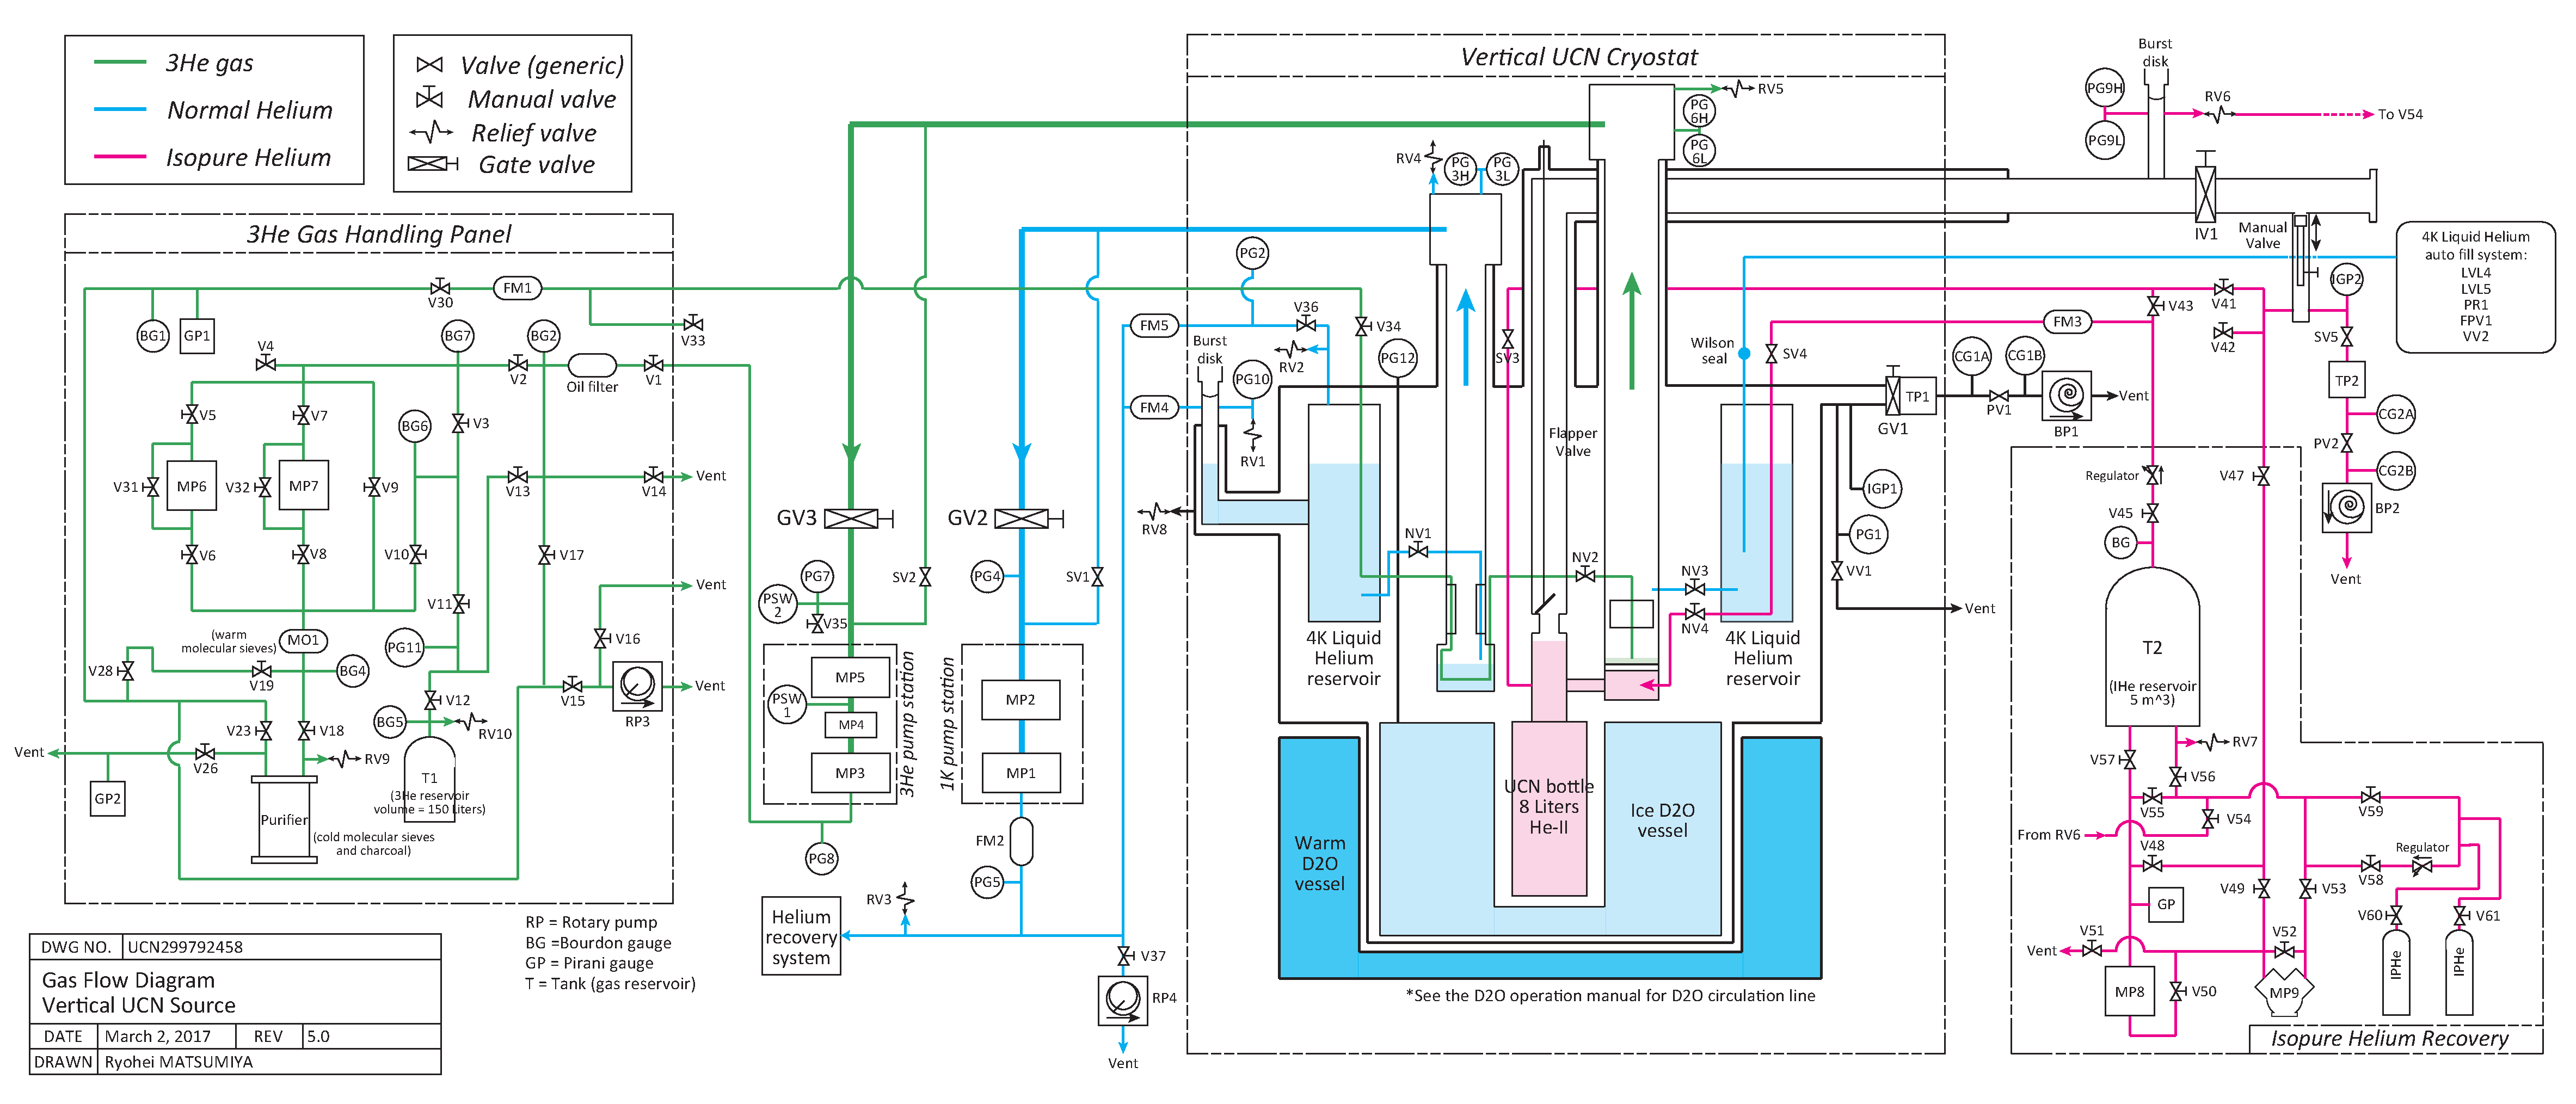
\includegraphics[width=1.05\textwidth, angle = 270]{gasflow.pdf}
    \caption{ Gas flow diagram for the vertical UCN source }
    \label{fig:gasflow}
\end{figure}
%  \chapter{Heat Conductivity in Superfluid Helium and Heater Tests~\label{sec:heattest}~\cite{Florian_thesis}}

%The cooling process of the spallation neutrons creates a heat input on
%the cryostat. This heat input must be removed to keep the temperature
%of the superfluid helium constant. This is critical, since the storage
%lifetime of UCN depend strongly on the superfluid helium temperature.

There are several sources of heat input on the UCN cryostat such as
the cooling process or the target irradiation. The heat load on the
UCN cryostat creates a temperature gradient along the heat exchanger
to the suprefluid helium bottle~(see Fig.~\ref{fig:gasflow}. The
temperature gradient in the superfluid helium is described by its heat
conductivity. Lower heat conductivities give rise to larger
temperature gradients.

The temperature dependence of the heat conductivity in the superfluid
helium is describe by theorical models from the lambda point at 2.17~K
down to around 1.4~K which is above the temperatures for the UCN
production~($<~1$~K). Since it is difficult to reach such low
temperatures, the mechanism of heat transfer in temperatures below
1.4~K is not fully understood.  To check the validity of the
theoretical models, here the extrapolation to lower temperatures is
compared to the acquired data with the vertical UCN source.


In order to create a temperature gradient along the channel from heat
exchanger to the superfluid helium bottle, the heater tapes that are
wrapped around the superfluid helium bottle are used.
%These heaters can
%create a temperature gradient between the heat exchanger and the
%superfluid helium bottle~(see Sec.~\ref{sec:vertical_source}).
This temperature gradient can be measured using the temperature
sensors shown in Fig.~\ref{fig:TSs}.

The heater test procedure is the following; The heater tape around the
superfluid helium bottle is turned on when the temperature of the
superfluid helium is stable. Here this temperature is refered to as
the {\it{base}} temperature. The applied heat load could easily be
calculated since the applied current and voltage are known. After the
heater is turned on, the temperature of the superfluid helium starts
to increase. This causes an increase in the flow rate in the $^3$He
pot. After some time, the temperature of the superfluid helium starts
to settle and reach a new equilibrium. This temperature is referred to
as the {\it{saturation}} temperature. At this point, the heater could
be turned off which causes the superfluid temperature and the flow
rate of the $^3$He to get back to the initial conditions.

In 2017, two sets of heater tests were performed on the vertical UCN
source: The April heat test and the November heat test. In April, the
base temperature of the superfluid helium was slightly higher than in
November. In addition, there was no proton beam during the April
cooling of the cryostat and it was purely a cryostat cooling
test. Table.~\ref{tab:heattest} shows the heat load and the
temperatures of the superfluid helium for those tests.

\begin{sidewaystable}
  %\centering
  \begin{tabular}{|c|c|c|c|c|c|c|c|c|c|c|}
    \hline
    Heater Power & T$_{\mathrm{base, TS10}}$ &  T$_{\mathrm{sat., TS10}}$ & T$_{\mathrm{base, TS11}}$ &  T$_{\mathrm{sat., TS11}}$ & T$_{\mathrm{base, TS12}}$ &  T$_{\mathrm{sat., TS12}}$ & T$_{\mathrm{base, TS14}}$ &  T$_{\mathrm{sat., TS14}}$ & T$_{\mathrm{base, TS16}}$ &  T$_{\mathrm{sat., TS16}}$ \\
    (mW) & (K) & (K) & (K) & (K) & (K) & (K) & (K) & (K) & (K) & (K) \\
    \hline
    \hline
    \multicolumn{11}{|c|}{\textbf{April Heat Test}}\\
    \hline
   2.5 & 0.717 & 0.718 & 0.93 & 0.931 & 0.926 & 0.9271 & 0.93 & 0.931 & 1.012 & 1.013 \\
    \hline
    12.5 & 0.717 & 0.7185 & 0.93 &  0.9315 & 0.924 & 0.929 & 0.93 & 0.9315 & 1.011 & 1.015 \\
    \hline
    25 & 0.719 & 0.723 & 0.928 & 0.931 & 0.919 & 0.929 & 0.928 & 0.931 & 1.008 & 1.015 \\
    \hline
    75 & 0.7195 & 0.7255 & 0.9285 & 0.937 & 0.922 & 0.952 & 0.928 & 0.937 & 1.01 & 1.03 \\
    \hline
    250 & 0.7175 & 0.7375 & 0.93 & 0.9475 & 0.93 & 1 & 0.93 & 0.947 & 1.01 & 1.065 \\
    \hline
    \multicolumn{11}{|c|}{\textbf{November Heat Test}}\\
    \hline
   25 & 0.724 & 0.73 & 0.892 & 0.9 & 0.84 & 0.86 & 0.92 & 0.923 & 0.96 & 0.97 \\
    \hline
    50 & 0.741 & 0.75 & 0.895 & 0.91 & 0.84 & 0.9 & 0.92 & 0.93 & 0.96 & 0.99 \\
    \hline
    75 & 0.73 & 0.74 & 0.9 & 0.91 & 0.85 & 0.92 & 0.92 & 0.93 & 0.96 & 1 \\
    \hline
    100 & 0.73 & 0.769 & 0.9 & 0.936 & 0.85 & 0.96 & 0.92 & 0.952 & 0.96 & 1.04 \\
    \hline
    150 & 0.73 & 0.755 & 0.9 & 0.93 & 0.84 & 0.99 & 0.92 & 0.945 & 0.96 & 1.06 \\
    \hline
    200 & 0.73 & 0.9 & 0.9 & 1.26 & 0.84 & 1.23 & 0.92 & 1.25 & 0.96 & 1.26 \\
    \hline
    250 & 0.73 & 0.94 & 0.895 & 1.385 & 0.84 & 1.345 & 0.92 & 1.363 & 0.97 & 1.375 \\
    \hline
  \end{tabular}
  \caption{The heater power, and the base and saturation temperatures
    from the temperature sensors in the superfluid helium, and in the
    $^3$He pot, for the April and November heat
    tests~\cite{Florian_thesis}}
  \label{tab:heattest}
\end{sidewaystable}


\subsection{Theoretical Models}
The relationship between the heat flux and the temperature gradient in
a one dimentional channel is written as

\begin{equation}
  \label{eqn:q_dT}
  q^m = f^{-1}\left(T, p \right) \frac{dT}{dx}
\end{equation}
where $q$ is the input heat flux, $T$ is the temperature, $p$ is the
pressure, $\frac{dT}{dx}$ is the temperature gradient along the
channel and $f\left(T, p \right)$ is the heat conductivity fucntion
which controls the temperature gradient of the heat flux which could
be written as
\begin{equation}
  \label{eqn:f}
f \left( T, p \right) = \frac{A_\mathrm{GM}\rho_n}{\rho_s^{3}s^4T^3}.
\end{equation}
Here $\rho_n$ is the density of the normal fluid component, $\rho_s$
is the density of the superfluid component, $s$ is the specific
entropy, $T$ is the temperature and $A_\mathrm{GM}$ is the
Gorter-Mellink parameter which describes the friction between the
normal fluid component and the superfluid component.

Since the Gorter-Mellink parameter is unknown, it is difficult to
calculate $f \left( T, p \right)$ in the form of
Eqn.~\ref{eqn:f}. However, there are other models to describe the
behaviour of the heat conductivity functions. There are two models
that are considered here at the saturated vapour pressure. This means,
the pressure dependence could be neglected. The models are the theory
model from Van Sciver~\cite{van2012helium} and the HEPAK
model~\cite{arp2005hepak}. %Fig.~\ref{fig:VanSciver_vs_HEPAK}

\begin{figure}[h!]
  \centering \includegraphics[width=0.8\textwidth]{VanSciver_vs_HEPAK.png}
  \caption{The heat conductivity function of the Van Sciver and HEPAK
    models. The vertical axis shows the temperature gradient along the
    channel and the horizonal axis shows the input heat
    flux~\cite{Florian_thesis}. The arrows on the graph indicate the
    temperature of the superfluid helium}
\label{fig:VanSciver_vs_HEPAK}
\end{figure}

The heat conductivity function for the Van Sciver and the HEPAK
theoretical models are shown in Fig.~\ref{fig:VanSciver_vs_HEPAK}. As
the graph shows, both models tend to agree at higher heat
inputs. However, at lower heat inputs, the heat conductivity function
values for the Van Sciver model lie below the values for the HEPAK
model. In addition, as the temperature of the superfluid helium
increases, the heat conductivity function tends to look more
linear. Since the Van Sciver model is more well known, it is used for
comparision with experimental data.

%%%%%%%%%%%%%%%%%%%%%%%%%%%%%%%%%%%%%%%%%%%%%%%%%%%%%%%%
\section{Measurement Result}
The data shown in Table.~\ref{tab:heattest} is a set of cleaned data
from all the heat tests in 2017. If the heat load on the cryostat is
higher than its cooling power, the temperature of the superfluid
helium would increase linearly without reaching an equilibrium. This
phenomena has been observed for higher heater powers e.g. 1~W. As a
result, that data is discarded.


Fig.~\ref{fig:April_Data} shows the result of the April heat test.
For a given heat input, the temperature difference between the base
and the saturation temperature for each temperature sensor is
calculated~(see table~\ref{tab:heattest}). The average of all of those
temperature differences give the overall $\Delta T$ across the
channel. Those are shown with black dots in Fig.~\ref{fig:April_Data}
as the raw data. However, the heat input for each data point should be
corrected since the total heat input is a combination of the added
heat from the heater tapes and the background heat load on the
cryostat which is not taken into account.


\begin{figure}[h!]
  \centering \includegraphics[width=0.8\textwidth]{April_Data.png}
  \caption{The comparison between the April heat test data and the Van
    Sciver model. The lines show the Van Sciver model's heat
    conductivity function at different superfluid helium bath
    temperatures. The black data points show the measured raw data of
    the heat tests. The blue points are the Joule Thomson values,
    which are the raw data plus the calculated background heat
    (included Joule-Thomson effect) and the red points show the raw
    data with the assumed 50 mW background heat input. }
\label{fig:April_Data}
\end{figure}


The two other sources of heat input to be considered are the
Joule-Thomson expansion and the the background heat load to the $^3$He
pot due to the thermal readiation and to the superfluid helium
bottle. The Joule-Thomson expansion happens when a gas or liquid
passes through a valve which has different temperature and pressures
on both sides while there is no heat exchange to the environment. Here
$^3$He flows into the heat exchanger and passes through a valve with
different pressures and temperatures on two sides. Because of the
Joule-Thomson expansion some liquid changes into vapor which is then
directly pumped out of the system and does not contribute to the
cooling process. For the backround heat load, based on estimations of
the sources of the background heat to the bottle alone, combined with
the measurements of the mass flow of $^4$He from the top of the bottle
when the $^3$He system is switched off, a heat of $\simeq$~50~mW is a
reasonable estimate of the true background heat to the bottle
alone. In Fig.~\ref{fig:April_Data}, the assumed values are the sum of
the 50~mW background heat and the heat input from the heaters and the
Joule-Thomson values are the sum of the heat input from the heaters
plus the calculated 232~mW calculated background
heat~\cite{Florian_thesis}.



Fig.~\ref{fig:November_Data} shows the data with the heaters in
November as well as the theoretical model of Van Sciver for the heat
conductivity. Each color represents a temperature range. The markers
are the actual data taken in November 2017.

At all the temperture ranges, the acquired data shows lower heat load
compared to the theoretical model. At the range of 1.2-1.3~K, the data
point with the smaller $\Delta$T is acquired at a higher He-II base
temperature, whereas the data point with higher $\Delta$T is acquired
at standard He-II base temperature. The data points which are closer
to the theoretical models are acquired at lower base temperature for
the superfluid helium. Since the measured data show bigger temperature
differences compared to the theoretical model of Van Sciver, it
suggests that the theory is assuming higher heat conductivity. Looking
back at Fig.~\ref{fig:VanSciver_vs_HEPAK}, it shows that using the
HEPAK model might solve this problem since the HEPAK model shows lower
heat conductivity.

One reason between the disagreement between the measurements and
theory could be the fact that these theoretical models are only
measured down to 1.4~K and they are extrapolated to lower
temperatures. Another reason could lie in the geometry difference. The
theoretical models are valid for a one-dimensional channel while there
is a 90$^\circ$ bend in the experimental setup~(see
Fig.~\ref{what???}) which can cause a higher temperature differnece
across the channel. One other reason might be the uncertainty in the
measured temperature due to the calibration of the temperature
sesnors. There might be other unknown sources of systematic error
affecting the measurements.


\begin{figure}[h!]
  \centering \includegraphics[width=0.8\textwidth]{November_Data.png}
  \caption{Theoretical model of Van Sciver for the heat conductivity
    at different temperature ranges and the November data. The
    vertical axis shows the temperature difference between the base
    and the saturation temperature for temperature sensors. The
    horizontal axis shows the heat input from the heaters plus the
    background heat.}
\label{fig:November_Data}
\end{figure}


\end{appendices}




%\nocite{apsrev41Control}
%\bibliography{my-bib,revtex-custom}
\bibliographystyle{apsrev4-1}
%\bibliographystyle{unsrt}
\bibliography{mybib}

\end{document}
